\pdfoutput=1
% ---------------------------------------------------------------------------
% Complexity concentration as a god-class and god-method detector:
% a pre-registered test of a scale-free outlier rule against tool definitions
% and human labels.
%
% Built for arXiv (primary class cs.SE). Everything it needs is either a standard
% LaTeX package that arXiv's TeX Live already carries, or a file in this
% directory. There is no .bib: the bibliography is a `thebibliography`
% environment at the end, so no BibTeX pass and no .bbl upload is required.
%
% Every number in this file is a macro from generated/numbers.tex and every
% table is a fragment under generated/, both written by paper/scripts/tables.py
% from the harness's analysis files; the figures are drawn by
% paper/scripts/figures.py. Nothing numeric is typed by hand. See README.md.
%
% Build:   pdflatex main && pdflatex main       (twice, for the references)
% ---------------------------------------------------------------------------
\documentclass[11pt,a4paper]{article}

\usepackage[T1]{fontenc}
\usepackage[utf8]{inputenc}
\usepackage{lmodern}
\usepackage[margin=2.4cm]{geometry}
\usepackage{graphicx}
\usepackage{booktabs}
\usepackage{multirow}
\usepackage{amsmath}
\usepackage{microtype}
\usepackage[hidelinks]{hyperref}
\usepackage{caption}
\captionsetup{font=small,labelfont=bf}

% generated by paper/scripts/tables.py; do not edit
\newcommand{\agrBlobAbsExtraDiff}{+0.136}
\newcommand{\agrBlobAbsExtraDiffCI}{[+0.059, +0.225]}
\newcommand{\agrBlobAbsExtraReading}{reviewers call the extra flags positive more often than unflagged non-god units}
\newcommand{\agrBlobAbsFlagged}{242}
\newcommand{\agrBlobAbsMcc}{+0.220}
\newcommand{\agrBlobAbsMccCI}{[+0.162, +0.284]}
\newcommand{\agrBlobAbsPrecision}{0.29}
\newcommand{\agrBlobAbsRecall}{0.34}
\newcommand{\agrBlobBaseRate}{11.2\%}
\newcommand{\agrBlobDecorBlobFlagged}{335}
\newcommand{\agrBlobDecorBlobMcc}{+0.196}
\newcommand{\agrBlobDecorBlobMccCI}{[+0.142, +0.256]}
\newcommand{\agrBlobDecorBlobPrecision}{0.24}
\newcommand{\agrBlobDecorBlobRecall}{0.40}
\newcommand{\agrBlobGrpAbsN}{242}
\newcommand{\agrBlobGrpAbsNotToolN}{100}
\newcommand{\agrBlobGrpAbsNotToolPos}{21}
\newcommand{\agrBlobGrpAbsNotToolRate}{21.0\%}
\newcommand{\agrBlobGrpAbsPos}{70}
\newcommand{\agrBlobGrpAbsRate}{28.9\%}
\newcommand{\agrBlobGrpNeitherAbsNorToolN}{1491}
\newcommand{\agrBlobGrpNeitherAbsNorToolPos}{110}
\newcommand{\agrBlobGrpNeitherAbsNorToolRate}{7.4\%}
\newcommand{\agrBlobGrpNeitherRelNorToolN}{1408}
\newcommand{\agrBlobGrpNeitherRelNorToolPos}{100}
\newcommand{\agrBlobGrpNeitherRelNorToolRate}{7.1\%}
\newcommand{\agrBlobGrpRelN}{326}
\newcommand{\agrBlobGrpRelNotToolN}{183}
\newcommand{\agrBlobGrpRelNotToolPos}{31}
\newcommand{\agrBlobGrpRelNotToolRate}{16.9\%}
\newcommand{\agrBlobGrpRelPos}{81}
\newcommand{\agrBlobGrpRelRate}{24.8\%}
\newcommand{\agrBlobGrpToolN}{236}
\newcommand{\agrBlobGrpToolPos}{73}
\newcommand{\agrBlobGrpToolRate}{30.9\%}
\newcommand{\agrBlobPmdGodclassFlagged}{236}
\newcommand{\agrBlobPmdGodclassMcc}{+0.242}
\newcommand{\agrBlobPmdGodclassMccCI}{[+0.186, +0.301]}
\newcommand{\agrBlobPmdGodclassPrecision}{0.31}
\newcommand{\agrBlobPmdGodclassRecall}{0.36}
\newcommand{\agrBlobPos}{204}
\newcommand{\agrBlobRelExtraDiff}{+0.098}
\newcommand{\agrBlobRelExtraDiffCI}{[+0.045, +0.159]}
\newcommand{\agrBlobRelExtraReading}{reviewers call the extra flags positive more often than unflagged non-god units}
\newcommand{\agrBlobRelFlagged}{326}
\newcommand{\agrBlobRelMcc}{+0.202}
\newcommand{\agrBlobRelMccCI}{[+0.153, +0.254]}
\newcommand{\agrBlobRelMinusAbs}{-0.018}
\newcommand{\agrBlobRelMinusAbsCI}{[-0.058, +0.023]}
\newcommand{\agrBlobRelMinusAbsReading}{no difference resolved}
\newcommand{\agrBlobRelMinusDecorBlob}{+0.007}
\newcommand{\agrBlobRelMinusDecorBlobCI}{[-0.055, +0.071]}
\newcommand{\agrBlobRelMinusDecorBlobReading}{no difference resolved}
\newcommand{\agrBlobRelMinusPmdGodclass}{-0.039}
\newcommand{\agrBlobRelMinusPmdGodclassCI}{[-0.098, +0.020]}
\newcommand{\agrBlobRelMinusPmdGodclassReading}{no difference resolved}
\newcommand{\agrBlobRelMinusWmcFourSeven}{-0.023}
\newcommand{\agrBlobRelMinusWmcFourSevenCI}{[-0.079, +0.032]}
\newcommand{\agrBlobRelMinusWmcFourSevenReading}{no difference resolved}
\newcommand{\agrBlobRelPrecision}{0.25}
\newcommand{\agrBlobRelRecall}{0.40}
\newcommand{\agrBlobRepos}{390}
\newcommand{\agrBlobUnits}{1{,}827}
\newcommand{\agrBlobWmcFourSevenFlagged}{398}
\newcommand{\agrBlobWmcFourSevenMcc}{+0.226}
\newcommand{\agrBlobWmcFourSevenMccCI}{[+0.171, +0.283]}
\newcommand{\agrBlobWmcFourSevenPrecision}{0.25}
\newcommand{\agrBlobWmcFourSevenRecall}{0.48}
\newcommand{\agrComputedUtc}{2026-10-22 10:04:06 UTC}
\newcommand{\agrLmAbsExtraDiff}{+0.911}
\newcommand{\agrLmAbsExtraDiffCI}{[+0.897, +0.925]}
\newcommand{\agrLmAbsExtraReading}{reviewers call the extra flags positive more often than unflagged non-god units}
\newcommand{\agrLmAbsFlagged}{45}
\newcommand{\agrLmAbsMcc}{+0.421}
\newcommand{\agrLmAbsMccCI}{[+0.354, +0.485]}
\newcommand{\agrLmAbsPrecision}{0.98}
\newcommand{\agrLmAbsRecall}{0.20}
\newcommand{\agrLmBaseRate}{11.1\%}
\newcommand{\agrLmBrainMethodFlagged}{4}
\newcommand{\agrLmBrainMethodMcc}{+0.127}
\newcommand{\agrLmBrainMethodMccCI}{[+0.060, +0.189]}
\newcommand{\agrLmBrainMethodPrecision}{1.00}
\newcommand{\agrLmBrainMethodRecall}{0.02}
\newcommand{\agrLmCcOneFourFlagged}{47}
\newcommand{\agrLmCcOneFourMcc}{+0.420}
\newcommand{\agrLmCcOneFourMccCI}{[+0.353, +0.485]}
\newcommand{\agrLmCcOneFourPrecision}{0.96}
\newcommand{\agrLmCcOneFourRecall}{0.20}
\newcommand{\agrLmCognitiveOneFiveFlagged}{102}
\newcommand{\agrLmCognitiveOneFiveMcc}{+0.565}
\newcommand{\agrLmCognitiveOneFiveMccCI}{[+0.497, +0.629]}
\newcommand{\agrLmCognitiveOneFivePrecision}{0.87}
\newcommand{\agrLmCognitiveOneFiveRecall}{0.40}
\newcommand{\agrLmGrpAbsN}{45}
\newcommand{\agrLmGrpAbsNotToolN}{22}
\newcommand{\agrLmGrpAbsNotToolPos}{22}
\newcommand{\agrLmGrpAbsNotToolRate}{100.0\%}
\newcommand{\agrLmGrpAbsPos}{44}
\newcommand{\agrLmGrpAbsRate}{97.8\%}
\newcommand{\agrLmGrpNeitherAbsNorToolN}{1938}
\newcommand{\agrLmGrpNeitherAbsNorToolPos}{172}
\newcommand{\agrLmGrpNeitherAbsNorToolRate}{8.9\%}
\newcommand{\agrLmGrpNeitherRelNorToolN}{1783}
\newcommand{\agrLmGrpNeitherRelNorToolPos}{87}
\newcommand{\agrLmGrpNeitherRelNorToolRate}{4.9\%}
\newcommand{\agrLmGrpRelN}{205}
\newcommand{\agrLmGrpRelNotToolN}{177}
\newcommand{\agrLmGrpRelNotToolPos}{107}
\newcommand{\agrLmGrpRelNotToolRate}{60.5\%}
\newcommand{\agrLmGrpRelPos}{133}
\newcommand{\agrLmGrpRelRate}{64.9\%}
\newcommand{\agrLmGrpToolN}{28}
\newcommand{\agrLmGrpToolPos}{26}
\newcommand{\agrLmGrpToolRate}{92.9\%}
\newcommand{\agrLmLocFiveZeroFlagged}{68}
\newcommand{\agrLmLocFiveZeroMcc}{+0.481}
\newcommand{\agrLmLocFiveZeroMccCI}{[+0.412, +0.542]}
\newcommand{\agrLmLocFiveZeroPrecision}{0.91}
\newcommand{\agrLmLocFiveZeroRecall}{0.28}
\newcommand{\agrLmPmdMethodNpathTwoZeroZeroFlagged}{28}
\newcommand{\agrLmPmdMethodNpathTwoZeroZeroMcc}{+0.312}
\newcommand{\agrLmPmdMethodNpathTwoZeroZeroMccCI}{[+0.244, +0.371]}
\newcommand{\agrLmPmdMethodNpathTwoZeroZeroPrecision}{0.93}
\newcommand{\agrLmPmdMethodNpathTwoZeroZeroRecall}{0.12}
\newcommand{\agrLmPos}{220}
\newcommand{\agrLmRelExtraDiff}{+0.556}
\newcommand{\agrLmRelExtraDiffCI}{[+0.470, +0.636]}
\newcommand{\agrLmRelExtraReading}{reviewers call the extra flags positive more often than unflagged non-god units}
\newcommand{\agrLmRelFlagged}{205}
\newcommand{\agrLmRelMcc}{+0.582}
\newcommand{\agrLmRelMccCI}{[+0.517, +0.641]}
\newcommand{\agrLmRelMinusAbs}{+0.161}
\newcommand{\agrLmRelMinusAbsCI}{[+0.081, +0.240]}
\newcommand{\agrLmRelMinusAbsReading}{relative rule higher}
\newcommand{\agrLmRelMinusBrainMethod}{+0.454}
\newcommand{\agrLmRelMinusBrainMethodCI}{[+0.367, +0.550]}
\newcommand{\agrLmRelMinusBrainMethodReading}{relative rule higher}
\newcommand{\agrLmRelMinusCcOneFour}{+0.162}
\newcommand{\agrLmRelMinusCcOneFourCI}{[+0.085, +0.238]}
\newcommand{\agrLmRelMinusCcOneFourReading}{relative rule higher}
\newcommand{\agrLmRelMinusCognitiveOneFive}{+0.017}
\newcommand{\agrLmRelMinusCognitiveOneFiveCI}{[-0.050, +0.085]}
\newcommand{\agrLmRelMinusCognitiveOneFiveReading}{no difference resolved}
\newcommand{\agrLmRelMinusLocFiveZero}{+0.101}
\newcommand{\agrLmRelMinusLocFiveZeroCI}{[+0.025, +0.178]}
\newcommand{\agrLmRelMinusLocFiveZeroReading}{relative rule higher}
\newcommand{\agrLmRelMinusPmdMethodNpathTwoZeroZero}{+0.270}
\newcommand{\agrLmRelMinusPmdMethodNpathTwoZeroZeroCI}{[+0.193, +0.352]}
\newcommand{\agrLmRelMinusPmdMethodNpathTwoZeroZeroReading}{relative rule higher}
\newcommand{\agrLmRelPrecision}{0.65}
\newcommand{\agrLmRelRecall}{0.60}
\newcommand{\agrLmRepos}{392}
\newcommand{\agrLmUnits}{1{,}988}
\newcommand{\analysedUtc}{2026-10-18 22:18:48 UTC}
\newcommand{\analysisSha}{1f8e2bfa05f1}
\newcommand{\anonJs}{28\%}
\newcommand{\anonTs}{38\%}
\newcommand{\brainAbsFlagged}{21{,}652}
\newcommand{\brainAbsFp}{18{,}356}
\newcommand{\brainAbsFpGodFree}{57}
\newcommand{\brainAbsFpr}{0.016}
\newcommand{\brainAbsFprPct}{1.6\%}
\newcommand{\brainAbsMacroMcc}{0.387}
\newcommand{\brainAbsMeanFlagsGodFree}{1.5}
\newcommand{\brainAbsMicroMcc}{0.361}
\newcommand{\brainAbsPooledFprPct}{2.3\%}
\newcommand{\brainAbsPrecision}{0.15}
\newcommand{\brainAbsRecall}{0.88}
\newcommand{\brainAbsTp}{3{,}296}
\newcommand{\brainAucMacro}{0.985}
\newcommand{\brainAucMacroCI}{[0.972, 0.995]}
\newcommand{\brainAucMacroN}{79}
\newcommand{\brainCarryCo}{145}
\newcommand{\brainCut}{38}
\newcommand{\brainMacroFpr}{+0.087}
\newcommand{\brainMacroFprCI}{[+0.078, +0.096]}
\newcommand{\brainMacroFprVerdict}{inferior}
\newcommand{\brainMacroMcc}{-0.322}
\newcommand{\brainMacroMccCI}{[-0.355, -0.290]}
\newcommand{\brainMacroMccVerdict}{inferior}
\newcommand{\brainMargin}{0.066}
\newcommand{\brainMicroMcc}{-0.172}
\newcommand{\brainMicroMccCI}{[-0.292, -0.095]}
\newcommand{\brainMicroMccVerdict}{inferior}
\newcommand{\brainMinPosCo}{79}
\newcommand{\brainNGodFree}{39}
\newcommand{\brainNNeg}{814{,}203}
\newcommand{\brainNPos}{3{,}733}
\newcommand{\brainPooledAucDiff}{-0.003}
\newcommand{\brainPooledAucDiffCI}{[-0.010, +0.010]}
\newcommand{\brainPooledAucRaw}{0.984}
\newcommand{\brainPooledAucReading}{no difference resolved}
\newcommand{\brainPooledAucStd}{0.981}
\newcommand{\brainPosCo}{3{,}733}
\newcommand{\brainRelFlagged}{88{,}363}
\newcommand{\brainRelFp}{84{,}724}
\newcommand{\brainRelFpGodFree}{1906}
\newcommand{\brainRelFpr}{0.103}
\newcommand{\brainRelFprPct}{10.3\%}
\newcommand{\brainRelMacroMcc}{0.152}
\newcommand{\brainRelMeanFlagsGodFree}{48.9}
\newcommand{\brainRelMicroMcc}{0.189}
\newcommand{\brainRelPooledFprPct}{10.4\%}
\newcommand{\brainRelPrecision}{0.04}
\newcommand{\brainRelRecall}{0.97}
\newcommand{\brainRelTp}{3{,}639}
\newcommand{\brainSignal}{\texttt{cognitive}}
\newcommand{\brainVerdict}{inferior}
\newcommand{\brainZCut}{13.60}
\newcommand{\calibCcAuc}{0.997}
\newcommand{\calibCcRho}{0.95}
\newcommand{\calibCognitiveAuc}{0.999}
\newcommand{\calibCognitiveRho}{0.97}
\newcommand{\calibNlocAuc}{0.999}
\newcommand{\calibNlocRho}{0.92}
\newcommand{\cpFailed}{12}
\newcommand{\cpFlips}{26}
\newcommand{\cpMaxFlips}{23}
\newcommand{\cpMaxFlipsRepo}{Anuken/Mindustry}
\newcommand{\cpRate}{6.7\%}
\newcommand{\cpRepos}{10}
\newcommand{\cpSkipped}{7}
\newcommand{\cpTried}{29}
\newcommand{\cpUnion}{390}
\newcommand{\cpWithinBound}{within}
\newcommand{\decorAbsFlagged}{7{,}561}
\newcommand{\decorAbsFp}{5{,}156}
\newcommand{\decorAbsFpGodFree}{747}
\newcommand{\decorAbsFpr}{0.112}
\newcommand{\decorAbsFprPct}{11.2\%}
\newcommand{\decorAbsMacroMcc}{0.224}
\newcommand{\decorAbsMeanFlagsGodFree}{67.9}
\newcommand{\decorAbsMicroMcc}{0.261}
\newcommand{\decorAbsPooledFprPct}{9.5\%}
\newcommand{\decorAbsPrecision}{0.32}
\newcommand{\decorAbsRecall}{0.38}
\newcommand{\decorAbsTp}{2{,}405}
\newcommand{\decorAucGiven}{0.575}
\newcommand{\decorAucGivenCI}{[0.530, 0.624]}
\newcommand{\decorAucMacro}{0.737}
\newcommand{\decorAucMacroCI}{[0.704, 0.770]}
\newcommand{\decorAucMacroN}{69}
\newcommand{\decorCarryCo}{85}
\newcommand{\decorCut}{12}
\newcommand{\decorMacroFpr}{-0.033}
\newcommand{\decorMacroFprCI}{[-0.058, -0.011]}
\newcommand{\decorMacroFprVerdict}{superior}
\newcommand{\decorMacroMcc}{-0.023}
\newcommand{\decorMacroMccCI}{[-0.055, +0.006]}
\newcommand{\decorMacroMccVerdict}{non-inferior}
\newcommand{\decorMargin}{0.072}
\newcommand{\decorMicroMcc}{-0.032}
\newcommand{\decorMicroMccCI}{[-0.063, +0.001]}
\newcommand{\decorMicroMccVerdict}{non-inferior}
\newcommand{\decorMinPosCo}{69}
\newcommand{\decorNGodFree}{11}
\newcommand{\decorNNeg}{54{,}046}
\newcommand{\decorNPos}{6{,}382}
\newcommand{\decorPooledAucDiff}{+0.025}
\newcommand{\decorPooledAucDiffCI}{[-0.023, +0.065]}
\newcommand{\decorPooledAucRaw}{0.722}
\newcommand{\decorPooledAucReading}{no difference resolved}
\newcommand{\decorPooledAucStd}{0.747}
\newcommand{\decorPosCo}{6{,}382}
\newcommand{\decorRelFlagged}{6{,}131}
\newcommand{\decorRelFp}{4{,}196}
\newcommand{\decorRelFpGodFree}{716}
\newcommand{\decorRelFpr}{0.079}
\newcommand{\decorRelFprPct}{7.9\%}
\newcommand{\decorRelMacroMcc}{0.204}
\newcommand{\decorRelMeanFlagsGodFree}{65.1}
\newcommand{\decorRelMicroMcc}{0.230}
\newcommand{\decorRelPooledFprPct}{7.8\%}
\newcommand{\decorRelPrecision}{0.32}
\newcommand{\decorRelRecall}{0.30}
\newcommand{\decorRelTp}{1{,}935}
\newcommand{\decorSignal}{\texttt{cognitive\_max}}
\newcommand{\decorVerdict}{non-inferior}
\newcommand{\decorZCut}{2.12}
\newcommand{\filesGenerated}{1{,}875}
\newcommand{\filesOversize}{269}
\newcommand{\flagClassMadMax}{12.3\%}
\newcommand{\flagClassMadMaxLang}{c}
\newcommand{\flagClassMadMin}{8.4\%}
\newcommand{\flagClassMadMinLang}{go}
\newcommand{\flagMethodMadMax}{12.7\%}
\newcommand{\flagMethodMadMin}{7.7\%}
\newcommand{\fpAbsFpCoupledN}{791}
\newcommand{\fpAbsFpCoupledPct}{45.1\%}
\newcommand{\fpAbsFpCoupledPctCI}{[34.9\%, 54.8\%]}
\newcommand{\fpAbsFpDecorBlobN}{352}
\newcommand{\fpAbsFpDecorBlobPct}{20.1\%}
\newcommand{\fpAbsFpDecorBlobPctCI}{[14.6\%, 25.5\%]}
\newcommand{\fpAbsFpLargeClassN}{599}
\newcommand{\fpAbsFpLargeClassPct}{34.2\%}
\newcommand{\fpAbsFpLargeClassPctCI}{[25.6\%, 41.5\%]}
\newcommand{\fpAbsFpLowCohesionN}{1457}
\newcommand{\fpAbsFpLowCohesionPct}{83.1\%}
\newcommand{\fpAbsFpLowCohesionPctCI}{[65.0\%, 94.1\%]}
\newcommand{\fpAbsFpMedianNloc}{165}
\newcommand{\fpAbsFpMedianNom}{10}
\newcommand{\fpAbsFpMedianRaw}{30}
\newcommand{\fpAbsFpN}{1{,}753}
\newcommand{\fpAbsFpNeitherCoupledNorLowCohesionN}{258}
\newcommand{\fpAbsFpNeitherCoupledNorLowCohesionPct}{14.7\%}
\newcommand{\fpAbsFpNeitherCoupledNorLowCohesionPctCI}{[4.5\%, 31.7\%]}
\newcommand{\fpAbsFpNoneOfThreeN}{177}
\newcommand{\fpAbsFpNoneOfThreePct}{10.1\%}
\newcommand{\fpAbsFpNoneOfThreePctCI}{[4.1\%, 18.9\%]}
\newcommand{\fpAbsFpRepos}{64}
\newcommand{\fpAbsFpWmcFourSevenAndCoupledN}{436}
\newcommand{\fpAbsFpWmcFourSevenAndCoupledPct}{24.9\%}
\newcommand{\fpAbsFpWmcFourSevenAndCoupledPctCI}{[18.7\%, 31.1\%]}
\newcommand{\fpAbsFpWmcFourSevenN}{712}
\newcommand{\fpAbsFpWmcFourSevenPct}{40.6\%}
\newcommand{\fpAbsFpWmcFourSevenPctCI}{[35.4\%, 44.5\%]}
\newcommand{\fpComputedUtc}{2026-10-22 10:04:32 UTC}
\newcommand{\fpFnCoupledN}{851}
\newcommand{\fpFnCoupledPct}{66.8\%}
\newcommand{\fpFnCoupledPctCI}{[55.7\%, 74.1\%]}
\newcommand{\fpFnDecorBlobN}{873}
\newcommand{\fpFnDecorBlobPct}{68.5\%}
\newcommand{\fpFnDecorBlobPctCI}{[52.7\%, 80.0\%]}
\newcommand{\fpFnLargeClassN}{1035}
\newcommand{\fpFnLargeClassPct}{81.2\%}
\newcommand{\fpFnLargeClassPctCI}{[62.6\%, 91.6\%]}
\newcommand{\fpFnLowCohesionN}{1159}
\newcommand{\fpFnLowCohesionPct}{91.0\%}
\newcommand{\fpFnLowCohesionPctCI}{[71.8\%, 100.0\%]}
\newcommand{\fpFnMedianNloc}{272}
\newcommand{\fpFnMedianNom}{32}
\newcommand{\fpFnMedianRaw}{11}
\newcommand{\fpFnN}{1{,}274}
\newcommand{\fpFnNeitherCoupledNorLowCohesionN}{85}
\newcommand{\fpFnNeitherCoupledNorLowCohesionPct}{6.7\%}
\newcommand{\fpFnNeitherCoupledNorLowCohesionPctCI}{[0.0\%, 21.2\%]}
\newcommand{\fpFnNoneOfThreeN}{27}
\newcommand{\fpFnNoneOfThreePct}{2.1\%}
\newcommand{\fpFnNoneOfThreePctCI}{[0.0\%, 6.8\%]}
\newcommand{\fpFnRepos}{50}
\newcommand{\fpFnWmcFourSevenAndCoupledN}{803}
\newcommand{\fpFnWmcFourSevenAndCoupledPct}{63.0\%}
\newcommand{\fpFnWmcFourSevenAndCoupledPctCI}{[50.3\%, 71.2\%]}
\newcommand{\fpFnWmcFourSevenN}{1171}
\newcommand{\fpFnWmcFourSevenPct}{91.9\%}
\newcommand{\fpFnWmcFourSevenPctCI}{[85.6\%, 96.3\%]}
\newcommand{\fpFpCoupledN}{1650}
\newcommand{\fpFpCoupledPct}{38.5\%}
\newcommand{\fpFpCoupledPctCI}{[30.9\%, 46.9\%]}
\newcommand{\fpFpDecorBlobN}{688}
\newcommand{\fpFpDecorBlobPct}{16.0\%}
\newcommand{\fpFpDecorBlobPctCI}{[11.7\%, 20.2\%]}
\newcommand{\fpFpLargeClassN}{1119}
\newcommand{\fpFpLargeClassPct}{26.1\%}
\newcommand{\fpFpLargeClassPctCI}{[19.3\%, 31.9\%]}
\newcommand{\fpFpLowCohesionN}{3608}
\newcommand{\fpFpLowCohesionPct}{84.1\%}
\newcommand{\fpFpLowCohesionPctCI}{[66.5\%, 94.0\%]}
\newcommand{\fpFpMedianNloc}{113}
\newcommand{\fpFpMedianNom}{9}
\newcommand{\fpFpMedianRaw}{17}
\newcommand{\fpFpN}{4{,}288}
\newcommand{\fpFpNeitherCoupledNorLowCohesionN}{609}
\newcommand{\fpFpNeitherCoupledNorLowCohesionPct}{14.2\%}
\newcommand{\fpFpNeitherCoupledNorLowCohesionPctCI}{[4.9\%, 31.4\%]}
\newcommand{\fpFpNoneOfThreeN}{484}
\newcommand{\fpFpNoneOfThreePct}{11.3\%}
\newcommand{\fpFpNoneOfThreePctCI}{[4.7\%, 22.7\%]}
\newcommand{\fpFpRepos}{78}
\newcommand{\fpFpWmcFourSevenAndCoupledN}{628}
\newcommand{\fpFpWmcFourSevenAndCoupledPct}{14.6\%}
\newcommand{\fpFpWmcFourSevenAndCoupledPctCI}{[10.6\%, 20.4\%]}
\newcommand{\fpFpWmcFourSevenN}{1032}
\newcommand{\fpFpWmcFourSevenPct}{24.1\%}
\newcommand{\fpFpWmcFourSevenPctCI}{[18.4\%, 31.4\%]}
\newcommand{\fpKappaAuthorModel}{0.20}
\newcommand{\fpKappaAuthorModelAgree}{21}
\newcommand{\fpKappaAuthorModelN}{40}
\newcommand{\fpNeitherCoupledN}{4356}
\newcommand{\fpNeitherCoupledPct}{8.2\%}
\newcommand{\fpNeitherCoupledPctCI}{[5.9\%, 11.1\%]}
\newcommand{\fpNeitherDecorBlobN}{3563}
\newcommand{\fpNeitherDecorBlobPct}{6.7\%}
\newcommand{\fpNeitherDecorBlobPctCI}{[4.1\%, 9.7\%]}
\newcommand{\fpNeitherLargeClassN}{5870}
\newcommand{\fpNeitherLargeClassPct}{11.1\%}
\newcommand{\fpNeitherLargeClassPctCI}{[7.7\%, 13.9\%]}
\newcommand{\fpNeitherLowCohesionN}{41516}
\newcommand{\fpNeitherLowCohesionPct}{78.4\%}
\newcommand{\fpNeitherLowCohesionPctCI}{[59.0\%, 90.0\%]}
\newcommand{\fpNeitherMedianNloc}{27}
\newcommand{\fpNeitherMedianNom}{5}
\newcommand{\fpNeitherMedianRaw}{1}
\newcommand{\fpNeitherN}{52{,}960}
\newcommand{\fpNeitherNeitherCoupledNorLowCohesionN}{11317}
\newcommand{\fpNeitherNeitherCoupledNorLowCohesionPct}{21.4\%}
\newcommand{\fpNeitherNeitherCoupledNorLowCohesionPctCI}{[9.8\%, 40.7\%]}
\newcommand{\fpNeitherNoneOfThreeN}{11210}
\newcommand{\fpNeitherNoneOfThreePct}{21.2\%}
\newcommand{\fpNeitherNoneOfThreePctCI}{[9.8\%, 40.2\%]}
\newcommand{\fpNeitherRepos}{84}
\newcommand{\fpNeitherWmcFourSevenAndCoupledN}{628}
\newcommand{\fpNeitherWmcFourSevenAndCoupledPct}{1.2\%}
\newcommand{\fpNeitherWmcFourSevenAndCoupledPctCI}{[0.7\%, 1.8\%]}
\newcommand{\fpNeitherWmcFourSevenN}{1342}
\newcommand{\fpNeitherWmcFourSevenPct}{2.5\%}
\newcommand{\fpNeitherWmcFourSevenPctCI}{[1.7\%, 3.6\%]}
\newcommand{\fpReadAuthorFpGathererN}{15}
\newcommand{\fpReadAuthorFpGathererPct}{75\%}
\newcommand{\fpReadAuthorFpLeafN}{5}
\newcommand{\fpReadAuthorFpLeafPct}{25\%}
\newcommand{\fpReadAuthorFpN}{20}
\newcommand{\fpReadAuthorFpOtherN}{0}
\newcommand{\fpReadAuthorFpOtherPct}{0\%}
\newcommand{\fpReadAuthorFpTableN}{0}
\newcommand{\fpReadAuthorFpTablePct}{0\%}
\newcommand{\fpReadAuthorTpGathererN}{19}
\newcommand{\fpReadAuthorTpGathererPct}{95\%}
\newcommand{\fpReadAuthorTpLeafN}{1}
\newcommand{\fpReadAuthorTpLeafPct}{5\%}
\newcommand{\fpReadAuthorTpN}{20}
\newcommand{\fpReadAuthorTpOtherN}{0}
\newcommand{\fpReadAuthorTpOtherPct}{0\%}
\newcommand{\fpReadAuthorTpTableN}{0}
\newcommand{\fpReadAuthorTpTablePct}{0\%}
\newcommand{\fpReadModelFpGathererN}{17}
\newcommand{\fpReadModelFpGathererPct}{17\%}
\newcommand{\fpReadModelFpLeafN}{66}
\newcommand{\fpReadModelFpLeafPct}{66\%}
\newcommand{\fpReadModelFpN}{100}
\newcommand{\fpReadModelFpOtherN}{12}
\newcommand{\fpReadModelFpOtherPct}{12\%}
\newcommand{\fpReadModelFpTableN}{5}
\newcommand{\fpReadModelFpTablePct}{5\%}
\newcommand{\fpReadModelTpGathererN}{30}
\newcommand{\fpReadModelTpGathererPct}{30\%}
\newcommand{\fpReadModelTpLeafN}{58}
\newcommand{\fpReadModelTpLeafPct}{58\%}
\newcommand{\fpReadModelTpN}{100}
\newcommand{\fpReadModelTpOtherN}{10}
\newcommand{\fpReadModelTpOtherPct}{10\%}
\newcommand{\fpReadModelTpTableN}{2}
\newcommand{\fpReadModelTpTablePct}{2\%}
\newcommand{\fpRepos}{84}
\newcommand{\fpSampleFp}{100}
\newcommand{\fpSampleN}{200}
\newcommand{\fpSamplePerRepo}{3}
\newcommand{\fpSampleTp}{100}
\newcommand{\fpTpCoupledN}{1367}
\newcommand{\fpTpCoupledPct}{74.3\%}
\newcommand{\fpTpCoupledPctCI}{[59.0\%, 84.2\%]}
\newcommand{\fpTpDecorBlobN}{1247}
\newcommand{\fpTpDecorBlobPct}{67.7\%}
\newcommand{\fpTpDecorBlobPctCI}{[47.7\%, 80.4\%]}
\newcommand{\fpTpLargeClassN}{1373}
\newcommand{\fpTpLargeClassPct}{74.6\%}
\newcommand{\fpTpLargeClassPctCI}{[52.7\%, 88.0\%]}
\newcommand{\fpTpLowCohesionN}{1592}
\newcommand{\fpTpLowCohesionPct}{86.5\%}
\newcommand{\fpTpLowCohesionPctCI}{[62.3\%, 99.7\%]}
\newcommand{\fpTpMedianNloc}{415}
\newcommand{\fpTpMedianNom}{32}
\newcommand{\fpTpMedianRaw}{29}
\newcommand{\fpTpN}{1{,}841}
\newcommand{\fpTpNeitherCoupledNorLowCohesionN}{196}
\newcommand{\fpTpNeitherCoupledNorLowCohesionPct}{10.6\%}
\newcommand{\fpTpNeitherCoupledNorLowCohesionPctCI}{[0.2\%, 29.6\%]}
\newcommand{\fpTpNoneOfThreeN}{14}
\newcommand{\fpTpNoneOfThreePct}{0.8\%}
\newcommand{\fpTpNoneOfThreePctCI}{[0.0\%, 2.0\%]}
\newcommand{\fpTpRepos}{56}
\newcommand{\fpTpWmcFourSevenAndCoupledN}{1342}
\newcommand{\fpTpWmcFourSevenAndCoupledPct}{72.9\%}
\newcommand{\fpTpWmcFourSevenAndCoupledPctCI}{[57.9\%, 82.4\%]}
\newcommand{\fpTpWmcFourSevenN}{1782}
\newcommand{\fpTpWmcFourSevenPct}{96.8\%}
\newcommand{\fpTpWmcFourSevenPctCI}{[95.8\%, 98.0\%]}
\newcommand{\fpUnits}{60{,}363}
\newcommand{\friedRankAdjBoxplot}{3.85}
\newcommand{\friedRankDoubleMad}{2.67}
\newcommand{\friedRankIqr}{2.50}
\newcommand{\friedRankMadZ}{2.42}
\newcommand{\friedRankPctTopOne}{3.56}
\newcommand{\friedRulesCD}{0.53}
\newcommand{\friedRulesN}{131}
\newcommand{\friedSigRankCcMax}{3.02}
\newcommand{\friedSigRankCcMean}{4.92}
\newcommand{\friedSigRankCognitiveMax}{3.36}
\newcommand{\friedSigRankMiMean}{5.99}
\newcommand{\friedSigRankNlocSum}{1.19}
\newcommand{\friedSigRankNom}{2.52}
\newcommand{\friedSignalsCD}{0.75}
\newcommand{\friedSignalsN}{101}
\newcommand{\godOutsidePmd}{4}
\newcommand{\harnessCommit}{f9b26ba}
\newcommand{\humBlobAllAbsFlagged}{287}
\newcommand{\humBlobAllAbsFp}{226}
\newcommand{\humBlobAllAbsFpGodFree}{102}
\newcommand{\humBlobAllAbsFpr}{0.277}
\newcommand{\humBlobAllAbsFprPct}{27.7\%}
\newcommand{\humBlobAllAbsMacroMcc}{0.091}
\newcommand{\humBlobAllAbsMeanFlagsGodFree}{0.7}
\newcommand{\humBlobAllAbsMicroMcc}{0.252}
\newcommand{\humBlobAllAbsPooledFprPct}{28.8\%}
\newcommand{\humBlobAllAbsPrecision}{0.21}
\newcommand{\humBlobAllAbsRecall}{0.68}
\newcommand{\humBlobAllAbsTp}{61}
\newcommand{\humBlobAllAucMacro}{0.747}
\newcommand{\humBlobAllAucMacroCI}{[0.685, 0.812]}
\newcommand{\humBlobAllAucMacroN}{9}
\newcommand{\humBlobAllCut}{52.93}
\newcommand{\humBlobAllExploreLevel}{0.047}
\newcommand{\humBlobAllMacroFpr}{-0.271}
\newcommand{\humBlobAllMacroFprCI}{[-0.321, -0.225]}
\newcommand{\humBlobAllMacroFprVerdict}{superior}
\newcommand{\humBlobAllMacroMcc}{-0.284}
\newcommand{\humBlobAllMacroMccCI}{[-0.389, -0.186]}
\newcommand{\humBlobAllMacroMccVerdict}{inferior}
\newcommand{\humBlobAllMargin}{0.014}
\newcommand{\humBlobAllMicroMcc}{-0.228}
\newcommand{\humBlobAllMicroMccCI}{[-0.324, -0.115]}
\newcommand{\humBlobAllMicroMccVerdict}{inferior}
\newcommand{\humBlobAllMinPosCo}{9}
\newcommand{\humBlobAllMinPosEx}{9}
\newcommand{\humBlobAllNAucRepos}{9}
\newcommand{\humBlobAllNGodFree}{138}
\newcommand{\humBlobAllNNeg}{785}
\newcommand{\humBlobAllNPaired}{198}
\newcommand{\humBlobAllNPairedMacro}{60}
\newcommand{\humBlobAllNPos}{90}
\newcommand{\humBlobAllPooledAucDiff}{-0.022}
\newcommand{\humBlobAllPooledAucDiffCI}{[-0.042, -0.003]}
\newcommand{\humBlobAllPooledAucRaw}{0.787}
\newcommand{\humBlobAllPooledAucReading}{absolute ranking better}
\newcommand{\humBlobAllPooledAucStd}{0.765}
\newcommand{\humBlobAllPosCo}{90}
\newcommand{\humBlobAllPosEx}{118}
\newcommand{\humBlobAllPowered}{underpowered}
\newcommand{\humBlobAllRelFlagged}{5}
\newcommand{\humBlobAllRelFp}{4}
\newcommand{\humBlobAllRelFpGodFree}{2}
\newcommand{\humBlobAllRelFpr}{0.006}
\newcommand{\humBlobAllRelFprPct}{0.6\%}
\newcommand{\humBlobAllRelMacroMcc}{0.005}
\newcommand{\humBlobAllRelMeanFlagsGodFree}{0.0}
\newcommand{\humBlobAllRelMicroMcc}{0.024}
\newcommand{\humBlobAllRelPooledFprPct}{0.5\%}
\newcommand{\humBlobAllRelPrecision}{0.20}
\newcommand{\humBlobAllRelRecall}{0.01}
\newcommand{\humBlobAllRelTp}{1}
\newcommand{\humBlobAllReposCo}{198}
\newcommand{\humBlobAllReposEx}{194}
\newcommand{\humBlobAllRevCo}{875}
\newcommand{\humBlobAllRevEx}{978}
\newcommand{\humBlobAllSignal}{\texttt{mi\_max}}
\newcommand{\humBlobAllVerdict}{inferior}
\newcommand{\humBlobAllZCut}{1.03}
\newcommand{\humBlobLabelled}{223}
\newcommand{\humBlobMeasured}{208}
\newcommand{\humBlobPosAbsFlagged}{185}
\newcommand{\humBlobPosAbsFp}{124}
\newcommand{\humBlobPosAbsFpGodFree}{0}
\newcommand{\humBlobPosAbsFpr}{0.294}
\newcommand{\humBlobPosAbsFprPct}{29.4\%}
\newcommand{\humBlobPosAbsMacroMcc}{0.299}
\newcommand{\humBlobPosAbsMeanFlagsGodFree}{--}
\newcommand{\humBlobPosAbsMicroMcc}{0.297}
\newcommand{\humBlobPosAbsPooledFprPct}{30.5\%}
\newcommand{\humBlobPosAbsPrecision}{0.33}
\newcommand{\humBlobPosAbsRecall}{0.68}
\newcommand{\humBlobPosAbsTp}{61}
\newcommand{\humBlobPosAucMacro}{0.747}
\newcommand{\humBlobPosAucMacroCI}{[0.685, 0.812]}
\newcommand{\humBlobPosAucMacroN}{9}
\newcommand{\humBlobPosCut}{52.93}
\newcommand{\humBlobPosExploreLevel}{0.047}
\newcommand{\humBlobPosMacroFpr}{-0.292}
\newcommand{\humBlobPosMacroFprCI}{[-0.367, -0.217]}
\newcommand{\humBlobPosMacroFprVerdict}{superior}
\newcommand{\humBlobPosMacroMcc}{-0.284}
\newcommand{\humBlobPosMacroMccCI}{[-0.389, -0.186]}
\newcommand{\humBlobPosMacroMccVerdict}{inferior}
\newcommand{\humBlobPosMargin}{0.014}
\newcommand{\humBlobPosMicroMcc}{-0.266}
\newcommand{\humBlobPosMicroMccCI}{[-0.398, -0.134]}
\newcommand{\humBlobPosMicroMccVerdict}{inferior}
\newcommand{\humBlobPosMinPosCo}{9}
\newcommand{\humBlobPosMinPosEx}{9}
\newcommand{\humBlobPosNAucRepos}{9}
\newcommand{\humBlobPosNGodFree}{0}
\newcommand{\humBlobPosNNeg}{407}
\newcommand{\humBlobPosNPaired}{60}
\newcommand{\humBlobPosNPairedMacro}{60}
\newcommand{\humBlobPosNPos}{90}
\newcommand{\humBlobPosPooledAucDiff}{-0.008}
\newcommand{\humBlobPosPooledAucDiffCI}{[-0.030, +0.011]}
\newcommand{\humBlobPosPooledAucRaw}{0.770}
\newcommand{\humBlobPosPooledAucReading}{no difference resolved}
\newcommand{\humBlobPosPooledAucStd}{0.762}
\newcommand{\humBlobPosPosCo}{90}
\newcommand{\humBlobPosPosEx}{118}
\newcommand{\humBlobPosPowered}{underpowered}
\newcommand{\humBlobPosRelFlagged}{3}
\newcommand{\humBlobPosRelFp}{2}
\newcommand{\humBlobPosRelFpGodFree}{0}
\newcommand{\humBlobPosRelFpr}{0.003}
\newcommand{\humBlobPosRelFprPct}{0.2\%}
\newcommand{\humBlobPosRelMacroMcc}{0.015}
\newcommand{\humBlobPosRelMeanFlagsGodFree}{--}
\newcommand{\humBlobPosRelMicroMcc}{0.031}
\newcommand{\humBlobPosRelPooledFprPct}{0.5\%}
\newcommand{\humBlobPosRelPrecision}{0.33}
\newcommand{\humBlobPosRelRecall}{0.01}
\newcommand{\humBlobPosRelTp}{1}
\newcommand{\humBlobPosReposCo}{60}
\newcommand{\humBlobPosReposEx}{74}
\newcommand{\humBlobPosRevCo}{497}
\newcommand{\humBlobPosRevEx}{609}
\newcommand{\humBlobPosSignal}{\texttt{mi\_max}}
\newcommand{\humBlobPosVerdict}{inferior}
\newcommand{\humBlobPosZCut}{0.29}
\newcommand{\humBlobRevLabelled}{2085}
\newcommand{\humBlobRevMeasured}{1853}
\newcommand{\humBlobRevRate}{88.9\%}
\newcommand{\humComputedUtc}{2026-10-22 10:03:52 UTC}
\newcommand{\humLmLabelled}{239}
\newcommand{\humLmMeasured}{228}
\newcommand{\humLmRevLabelled}{2219}
\newcommand{\humLmRevMeasured}{2028}
\newcommand{\humLmRevRate}{91.4\%}
\newcommand{\humLongMethodAllAbsFlagged}{142}
\newcommand{\humLongMethodAllAbsFp}{39}
\newcommand{\humLongMethodAllAbsFpGodFree}{12}
\newcommand{\humLongMethodAllAbsFpr}{0.039}
\newcommand{\humLongMethodAllAbsFprPct}{3.9\%}
\newcommand{\humLongMethodAllAbsMacroMcc}{0.276}
\newcommand{\humLongMethodAllAbsMeanFlagsGodFree}{0.1}
\newcommand{\humLongMethodAllAbsMicroMcc}{0.785}
\newcommand{\humLongMethodAllAbsPooledFprPct}{4.7\%}
\newcommand{\humLongMethodAllAbsPrecision}{0.73}
\newcommand{\humLongMethodAllAbsRecall}{0.91}
\newcommand{\humLongMethodAllAbsTp}{103}
\newcommand{\humLongMethodAllAucMacro}{0.979}
\newcommand{\humLongMethodAllAucMacroCI}{[0.957, 0.997]}
\newcommand{\humLongMethodAllAucMacroN}{8}
\newcommand{\humLongMethodAllCut}{50.63}
\newcommand{\humLongMethodAllExploreLevel}{0.388}
\newcommand{\humLongMethodAllMacroFpr}{+0.032}
\newcommand{\humLongMethodAllMacroFprCI}{[+0.000, +0.069]}
\newcommand{\humLongMethodAllMacroFprVerdict}{inconclusive}
\newcommand{\humLongMethodAllMacroMcc}{-0.358}
\newcommand{\humLongMethodAllMacroMccCI}{[-0.473, -0.242]}
\newcommand{\humLongMethodAllMacroMccVerdict}{inferior}
\newcommand{\humLongMethodAllMargin}{0.100}
\newcommand{\humLongMethodAllMicroMcc}{-0.362}
\newcommand{\humLongMethodAllMicroMccCI}{[-0.492, -0.242]}
\newcommand{\humLongMethodAllMicroMccVerdict}{inferior}
\newcommand{\humLongMethodAllMinPosCo}{8}
\newcommand{\humLongMethodAllMinPosEx}{13}
\newcommand{\humLongMethodAllNAucRepos}{8}
\newcommand{\humLongMethodAllNGodFree}{123}
\newcommand{\humLongMethodAllNNeg}{835}
\newcommand{\humLongMethodAllNPaired}{192}
\newcommand{\humLongMethodAllNPairedMacro}{69}
\newcommand{\humLongMethodAllNPos}{113}
\newcommand{\humLongMethodAllPooledAucDiff}{-0.069}
\newcommand{\humLongMethodAllPooledAucDiffCI}{[-0.098, -0.046]}
\newcommand{\humLongMethodAllPooledAucRaw}{0.986}
\newcommand{\humLongMethodAllPooledAucReading}{absolute ranking better}
\newcommand{\humLongMethodAllPooledAucStd}{0.917}
\newcommand{\humLongMethodAllPosCo}{113}
\newcommand{\humLongMethodAllPosEx}{115}
\newcommand{\humLongMethodAllPowered}{underpowered}
\newcommand{\humLongMethodAllRelFlagged}{104}
\newcommand{\humLongMethodAllRelFp}{51}
\newcommand{\humLongMethodAllRelFpGodFree}{26}
\newcommand{\humLongMethodAllRelFpr}{0.071}
\newcommand{\humLongMethodAllRelFprPct}{7.1\%}
\newcommand{\humLongMethodAllRelMacroMcc}{0.148}
\newcommand{\humLongMethodAllRelMeanFlagsGodFree}{0.2}
\newcommand{\humLongMethodAllRelMicroMcc}{0.423}
\newcommand{\humLongMethodAllRelPooledFprPct}{6.1\%}
\newcommand{\humLongMethodAllRelPrecision}{0.51}
\newcommand{\humLongMethodAllRelRecall}{0.47}
\newcommand{\humLongMethodAllRelTp}{53}
\newcommand{\humLongMethodAllReposCo}{192}
\newcommand{\humLongMethodAllReposEx}{202}
\newcommand{\humLongMethodAllRevCo}{948}
\newcommand{\humLongMethodAllRevEx}{1080}
\newcommand{\humLongMethodAllSignal}{\texttt{mi}}
\newcommand{\humLongMethodAllVerdict}{inferior}
\newcommand{\humLongMethodAllZCut}{2.40}
\newcommand{\humLongMethodPosAbsFlagged}{130}
\newcommand{\humLongMethodPosAbsFp}{27}
\newcommand{\humLongMethodPosAbsFpGodFree}{0}
\newcommand{\humLongMethodPosAbsFpr}{0.034}
\newcommand{\humLongMethodPosAbsFprPct}{3.4\%}
\newcommand{\humLongMethodPosAbsMacroMcc}{0.769}
\newcommand{\humLongMethodPosAbsMeanFlagsGodFree}{--}
\newcommand{\humLongMethodPosAbsMicroMcc}{0.814}
\newcommand{\humLongMethodPosAbsPooledFprPct}{5.3\%}
\newcommand{\humLongMethodPosAbsPrecision}{0.79}
\newcommand{\humLongMethodPosAbsRecall}{0.91}
\newcommand{\humLongMethodPosAbsTp}{103}
\newcommand{\humLongMethodPosAucMacro}{0.979}
\newcommand{\humLongMethodPosAucMacroCI}{[0.957, 0.997]}
\newcommand{\humLongMethodPosAucMacroN}{8}
\newcommand{\humLongMethodPosCut}{50.63}
\newcommand{\humLongMethodPosExploreLevel}{0.388}
\newcommand{\humLongMethodPosMacroFpr}{+0.010}
\newcommand{\humLongMethodPosMacroFprCI}{[-0.019, +0.041]}
\newcommand{\humLongMethodPosMacroFprVerdict}{non-inferior}
\newcommand{\humLongMethodPosMacroMcc}{-0.358}
\newcommand{\humLongMethodPosMacroMccCI}{[-0.473, -0.242]}
\newcommand{\humLongMethodPosMacroMccVerdict}{inferior}
\newcommand{\humLongMethodPosMargin}{0.100}
\newcommand{\humLongMethodPosMicroMcc}{-0.325}
\newcommand{\humLongMethodPosMicroMccCI}{[-0.465, -0.185]}
\newcommand{\humLongMethodPosMicroMccVerdict}{inferior}
\newcommand{\humLongMethodPosMinPosCo}{8}
\newcommand{\humLongMethodPosMinPosEx}{13}
\newcommand{\humLongMethodPosNAucRepos}{8}
\newcommand{\humLongMethodPosNGodFree}{0}
\newcommand{\humLongMethodPosNNeg}{505}
\newcommand{\humLongMethodPosNPaired}{69}
\newcommand{\humLongMethodPosNPairedMacro}{69}
\newcommand{\humLongMethodPosNPos}{113}
\newcommand{\humLongMethodPosPooledAucDiff}{-0.057}
\newcommand{\humLongMethodPosPooledAucDiffCI}{[-0.098, -0.026]}
\newcommand{\humLongMethodPosPooledAucRaw}{0.987}
\newcommand{\humLongMethodPosPooledAucReading}{absolute ranking better}
\newcommand{\humLongMethodPosPooledAucStd}{0.929}
\newcommand{\humLongMethodPosPosCo}{113}
\newcommand{\humLongMethodPosPosEx}{115}
\newcommand{\humLongMethodPosPowered}{underpowered}
\newcommand{\humLongMethodPosRelFlagged}{78}
\newcommand{\humLongMethodPosRelFp}{25}
\newcommand{\humLongMethodPosRelFpGodFree}{0}
\newcommand{\humLongMethodPosRelFpr}{0.044}
\newcommand{\humLongMethodPosRelFprPct}{4.4\%}
\newcommand{\humLongMethodPosRelMacroMcc}{0.411}
\newcommand{\humLongMethodPosRelMeanFlagsGodFree}{--}
\newcommand{\humLongMethodPosRelMicroMcc}{0.488}
\newcommand{\humLongMethodPosRelPooledFprPct}{5.0\%}
\newcommand{\humLongMethodPosRelPrecision}{0.68}
\newcommand{\humLongMethodPosRelRecall}{0.47}
\newcommand{\humLongMethodPosRelTp}{53}
\newcommand{\humLongMethodPosReposCo}{69}
\newcommand{\humLongMethodPosReposEx}{59}
\newcommand{\humLongMethodPosRevCo}{618}
\newcommand{\humLongMethodPosRevEx}{592}
\newcommand{\humLongMethodPosSignal}{\texttt{mi}}
\newcommand{\humLongMethodPosVerdict}{inferior}
\newcommand{\humLongMethodPosZCut}{2.40}
\newcommand{\javaFilesCk}{85{,}931}
\newcommand{\javaFilesMulti}{19{,}952}
\newcommand{\javaFilesMultiPct}{23\%}
\newcommand{\mlcqAnalysedUtc}{2026-10-19 22:20:30 UTC}
\newcommand{\mlcqApacheShare}{50.2\%}
\newcommand{\mlcqBlob}{254}
\newcommand{\mlcqBlobReviewed}{2{,}334}
\newcommand{\mlcqBrainMicroMcc}{-0.166}
\newcommand{\mlcqBrainMicroMccCI}{[-0.333, -0.080]}
\newcommand{\mlcqBrainSignal}{\texttt{cognitive}}
\newcommand{\mlcqBrainVerdict}{inferior}
\newcommand{\mlcqDecorMicroMcc}{-0.082}
\newcommand{\mlcqDecorMicroMccCI}{[-0.115, -0.052]}
\newcommand{\mlcqDecorSignal}{\texttt{nloc\_max}}
\newcommand{\mlcqDecorVerdict}{inconclusive}
\newcommand{\mlcqErrors}{2}
\newcommand{\mlcqFlips}{5}
\newcommand{\mlcqHarnessCommit}{7b52774}
\newcommand{\mlcqLm}{276}
\newcommand{\mlcqLmReviewed}{2{,}430}
\newcommand{\mlcqNpathMicroMcc}{-0.262}
\newcommand{\mlcqNpathMicroMccCI}{[-0.290, -0.232]}
\newcommand{\mlcqNpathSignal}{\texttt{cc}}
\newcommand{\mlcqNpathVerdict}{inferior}
\newcommand{\mlcqOwners}{28}
\newcommand{\mlcqPmdAbsFlagged}{20{,}938}
\newcommand{\mlcqPmdAbsFp}{12{,}335}
\newcommand{\mlcqPmdAbsFpGodFree}{66}
\newcommand{\mlcqPmdAbsFpr}{0.080}
\newcommand{\mlcqPmdAbsFprPct}{8.0\%}
\newcommand{\mlcqPmdAbsMacroMcc}{0.355}
\newcommand{\mlcqPmdAbsMacroMccPos}{0.390}
\newcommand{\mlcqPmdAbsMeanFlagsGodFree}{3.0}
\newcommand{\mlcqPmdAbsMicroMcc}{0.483}
\newcommand{\mlcqPmdAbsPooledFprPct}{8.2\%}
\newcommand{\mlcqPmdAbsPrecision}{0.41}
\newcommand{\mlcqPmdAbsRecall}{0.69}
\newcommand{\mlcqPmdAbsTp}{8{,}603}
\newcommand{\mlcqPmdAucGiven}{0.619}
\newcommand{\mlcqPmdAucGivenCI}{[0.597, 0.640]}
\newcommand{\mlcqPmdAucMacro}{0.908}
\newcommand{\mlcqPmdAucMacroCI}{[0.900, 0.916]}
\newcommand{\mlcqPmdAucMacroN}{198}
\newcommand{\mlcqPmdCarryCo}{244}
\newcommand{\mlcqPmdCut}{17}
\newcommand{\mlcqPmdMacroFpr}{+0.007}
\newcommand{\mlcqPmdMacroFprCI}{[-0.005, +0.018]}
\newcommand{\mlcqPmdMacroFprVerdict}{non-inferior}
\newcommand{\mlcqPmdMacroMcc}{-0.020}
\newcommand{\mlcqPmdMacroMccCI}{[-0.039, -0.003]}
\newcommand{\mlcqPmdMacroMccPosN}{222}
\newcommand{\mlcqPmdMacroMccVerdict}{non-inferior}
\newcommand{\mlcqPmdMargin}{0.10}
\newcommand{\mlcqPmdMicroMcc}{-0.098}
\newcommand{\mlcqPmdMicroMccCI}{[-0.151, -0.063]}
\newcommand{\mlcqPmdMicroMccVerdict}{inconclusive}
\newcommand{\mlcqPmdMinPosCo}{198}
\newcommand{\mlcqPmdNGodFree}{22}
\newcommand{\mlcqPmdNNeg}{150{,}049}
\newcommand{\mlcqPmdNPos}{12{,}465}
\newcommand{\mlcqPmdPooledAucDiff}{-0.045}
\newcommand{\mlcqPmdPooledAucDiffCI}{[-0.080, -0.024]}
\newcommand{\mlcqPmdPooledAucRaw}{0.925}
\newcommand{\mlcqPmdPooledAucReading}{absolute ranking better}
\newcommand{\mlcqPmdPooledAucStd}{0.880}
\newcommand{\mlcqPmdPosCo}{12{,}465}
\newcommand{\mlcqPmdRelFlagged}{20{,}106}
\newcommand{\mlcqPmdRelFp}{13{,}083}
\newcommand{\mlcqPmdRelFpGodFree}{253}
\newcommand{\mlcqPmdRelFpr}{0.087}
\newcommand{\mlcqPmdRelFprPct}{8.7\%}
\newcommand{\mlcqPmdRelMacroMcc}{0.337}
\newcommand{\mlcqPmdRelMacroMccPos}{0.370}
\newcommand{\mlcqPmdRelMeanFlagsGodFree}{11.5}
\newcommand{\mlcqPmdRelMicroMcc}{0.385}
\newcommand{\mlcqPmdRelPooledFprPct}{8.7\%}
\newcommand{\mlcqPmdRelPrecision}{0.35}
\newcommand{\mlcqPmdRelRecall}{0.56}
\newcommand{\mlcqPmdRelTp}{7{,}023}
\newcommand{\mlcqPmdSignal}{\texttt{cognitive\_max}}
\newcommand{\mlcqPmdVerdict}{inconclusive}
\newcommand{\mlcqPmdZCut}{2.87}
\newcommand{\mlcqRepos}{522}
\newcommand{\mlcqRunDone}{499}
\newcommand{\mlcqRunFailed}{23}
\newcommand{\mlcqSamples}{4{,}764}
\newcommand{\mlcqTopOwner}{apache}
\newcommand{\mlcqTopOwnerN}{247}
\newcommand{\mlcqTotalFunctions}{4{,}541{,}402}
\newcommand{\mlcqUsable}{492}
\newcommand{\nJava}{171}
\newcommand{\nJavaMain}{30}
\newcommand{\nJavaSupp}{141}
\newcommand{\nMainSample}{304}
\newcommand{\nOwners}{430}
\newcommand{\nPilot}{522}
\newcommand{\nPilotOverlap}{1}
\newcommand{\nRowsSharingOwner}{23}
\newcommand{\nSupplement}{141}
\newcommand{\nUsable}{445}
\newcommand{\npathAbsFlagged}{4{,}278}
\newcommand{\npathAbsFp}{2{,}331}
\newcommand{\npathAbsFpGodFree}{16}
\newcommand{\npathAbsFpr}{0.005}
\newcommand{\npathAbsFprPct}{0.5\%}
\newcommand{\npathAbsMacroMcc}{0.434}
\newcommand{\npathAbsMeanFlagsGodFree}{0.8}
\newcommand{\npathAbsMicroMcc}{0.580}
\newcommand{\npathAbsPooledFprPct}{0.4\%}
\newcommand{\npathAbsPrecision}{0.46}
\newcommand{\npathAbsRecall}{0.75}
\newcommand{\npathAbsTp}{1{,}947}
\newcommand{\npathAucMacro}{0.996}
\newcommand{\npathAucMacroCI}{[0.994, 0.996]}
\newcommand{\npathAucMacroN}{51}
\newcommand{\npathCarryCo}{84}
\newcommand{\npathCut}{15}
\newcommand{\npathMacroFpr}{+0.052}
\newcommand{\npathMacroFprCI}{[+0.047, +0.057]}
\newcommand{\npathMacroFprVerdict}{inconclusive}
\newcommand{\npathMacroMcc}{-0.256}
\newcommand{\npathMacroMccCI}{[-0.308, -0.204]}
\newcommand{\npathMacroMccVerdict}{inferior}
\newcommand{\npathMargin}{0.098}
\newcommand{\npathMicroMcc}{-0.331}
\newcommand{\npathMicroMccCI}{[-0.380, -0.284]}
\newcommand{\npathMicroMccVerdict}{inferior}
\newcommand{\npathMinPosCo}{51}
\newcommand{\npathNGodFree}{21}
\newcommand{\npathNNeg}{587{,}282}
\newcommand{\npathNPos}{2{,}610}
\newcommand{\npathPooledAucDiff}{-0.004}
\newcommand{\npathPooledAucDiffCI}{[-0.007, -0.002]}
\newcommand{\npathPooledAucRaw}{0.997}
\newcommand{\npathPooledAucReading}{absolute ranking better}
\newcommand{\npathPooledAucStd}{0.993}
\newcommand{\npathPosCo}{2{,}610}
\newcommand{\npathRelFlagged}{38{,}363}
\newcommand{\npathRelFp}{35{,}782}
\newcommand{\npathRelFpGodFree}{652}
\newcommand{\npathRelFpr}{0.057}
\newcommand{\npathRelFprPct}{5.7\%}
\newcommand{\npathRelMacroMcc}{0.242}
\newcommand{\npathRelMeanFlagsGodFree}{31.0}
\newcommand{\npathRelMicroMcc}{0.250}
\newcommand{\npathRelPooledFprPct}{6.1\%}
\newcommand{\npathRelPrecision}{0.07}
\newcommand{\npathRelRecall}{0.99}
\newcommand{\npathRelTp}{2{,}581}
\newcommand{\npathSignal}{\texttt{cc}}
\newcommand{\npathVerdict}{inferior}
\newcommand{\npathZCut}{8.75}
\newcommand{\pilotOverlapRepo}{runkids/skillshare}
\newcommand{\pmdGodFreeShare}{22\%}
\newcommand{\pmdGodsMedian}{5}
\newcommand{\primAbsFlagged}{3{,}113}
\newcommand{\primAbsFp}{1{,}753}
\newcommand{\primAbsFpGodFree}{19}
\newcommand{\primAbsFpr}{0.038}
\newcommand{\primAbsFprPct}{3.8\%}
\newcommand{\primAbsMacroMcc}{0.285}
\newcommand{\primAbsMacroMccPos}{0.380}
\newcommand{\primAbsMeanFlagsGodFree}{0.9}
\newcommand{\primAbsMicroMcc}{0.406}
\newcommand{\primAbsPooledFprPct}{3.1\%}
\newcommand{\primAbsPrecision}{0.44}
\newcommand{\primAbsRecall}{0.44}
\newcommand{\primAbsTp}{1{,}360}
\newcommand{\primAucFloor}{0.70}
\newcommand{\primAucGiven}{0.624}
\newcommand{\primAucGivenCI}{[0.579, 0.672]}
\newcommand{\primAucMacro}{0.916}
\newcommand{\primAucMacroCI}{[0.903, 0.928]}
\newcommand{\primAucMacroN}{51}
\newcommand{\primBrKindApplicationAuc}{0.920}
\newcommand{\primBrKindApplicationMcc}{0.276}
\newcommand{\primBrKindApplicationN}{155}
\newcommand{\primBrKindLibraryAuc}{0.904}
\newcommand{\primBrKindLibraryMcc}{0.283}
\newcommand{\primBrKindLibraryN}{61}
\newcommand{\primBrTierHighAuc}{0.911}
\newcommand{\primBrTierHighMcc}{0.297}
\newcommand{\primBrTierHighN}{82}
\newcommand{\primBrTierLowAuc}{0.916}
\newcommand{\primBrTierLowMcc}{0.253}
\newcommand{\primBrTierLowN}{59}
\newcommand{\primBrTierMidAuc}{0.920}
\newcommand{\primBrTierMidMcc}{0.278}
\newcommand{\primBrTierMidN}{75}
\newcommand{\primCarryCo}{84}
\newcommand{\primCarryEx}{86}
\newcommand{\primCut}{22}
\newcommand{\primExploreAuc}{0.916}
\newcommand{\primExploreBestDensity}{\texttt{cognitive\_mean}}
\newcommand{\primExploreBestDensityAuc}{0.811}
\newcommand{\primExploreLevel}{0.399}
\newcommand{\primExploreSecond}{\texttt{nloc\_max}}
\newcommand{\primExploreSecondAuc}{0.893}
\newcommand{\primFlagRateAdjBoxplot}{2.1\%}
\newcommand{\primFlagRateDoubleMad}{5.9\%}
\newcommand{\primFlagRateEvtPot}{0.2\%}
\newcommand{\primFlagRateIqr}{9.1\%}
\newcommand{\primFlagRateMadZ}{10.6\%}
\newcommand{\primFlagRateMadz}{10.6\%}
\newcommand{\primFlagRatePctTopOne}{2.1\%}
\newcommand{\primFlagRateZscore}{2.2\%}
\newcommand{\primFprMargin}{0.05}
\newcommand{\primMacroFpr}{+0.042}
\newcommand{\primMacroFprCI}{[+0.027, +0.056]}
\newcommand{\primMacroFprN}{84}
\newcommand{\primMacroFprVerdict}{inconclusive}
\newcommand{\primMacroMcc}{-0.009}
\newcommand{\primMacroMccCI}{[-0.057, +0.040]}
\newcommand{\primMacroMccN}{63}
\newcommand{\primMacroMccPosN}{63}
\newcommand{\primMacroMccVerdict}{non-inferior}
\newcommand{\primMargin}{0.10}
\newcommand{\primMicroMcc}{-0.028}
\newcommand{\primMicroMccCI}{[-0.068, +0.005]}
\newcommand{\primMicroMccN}{84}
\newcommand{\primMicroMccVerdict}{non-inferior}
\newcommand{\primMinPosCo}{51}
\newcommand{\primMinPosEx}{50}
\newcommand{\primNGodFree}{21}
\newcommand{\primNNeg}{57{,}248}
\newcommand{\primNPos}{3{,}115}
\newcommand{\primPooledAucDiff}{-0.020}
\newcommand{\primPooledAucDiffCI}{[-0.033, -0.008]}
\newcommand{\primPooledAucRaw}{0.923}
\newcommand{\primPooledAucReading}{absolute ranking better}
\newcommand{\primPooledAucStd}{0.903}
\newcommand{\primPosCo}{3{,}115}
\newcommand{\primPosEx}{2{,}862}
\newcommand{\primRelFlagged}{6{,}129}
\newcommand{\primRelFp}{4{,}288}
\newcommand{\primRelFpGodFree}{139}
\newcommand{\primRelFpr}{0.079}
\newcommand{\primRelFprPct}{7.9\%}
\newcommand{\primRelMacroMcc}{0.278}
\newcommand{\primRelMacroMccPos}{0.371}
\newcommand{\primRelMeanFlagsGodFree}{6.6}
\newcommand{\primRelMicroMcc}{0.378}
\newcommand{\primRelPooledFprPct}{7.5\%}
\newcommand{\primRelPrecision}{0.30}
\newcommand{\primRelRecall}{0.59}
\newcommand{\primRelTp}{1{,}841}
\newcommand{\primReposCo}{216}
\newcommand{\primReposEx}{229}
\newcommand{\primSignal}{\texttt{cognitive\_max}}
\newcommand{\primVerdict}{inconclusive}
\newcommand{\primZCut}{2.75}
\newcommand{\reanalysedUtc}{2026-10-19 04:44:09 UTC}
\newcommand{\runDone}{446}
\newcommand{\runFailed}{2}
\newcommand{\sampleCrossStratumLangs}{8 to Python, 6 to Java, 5 to JavaScript, 5 to TypeScript, 2 to PHP, 2 to C++, 1 to Go, 1 to Rust}
\newcommand{\sampleCrossStratumN}{30}
\newcommand{\sampleFailedN}{1}
\newcommand{\sampleFailedRepos}{openjdk/jdk}
\newcommand{\sampleMainDrawn}{431}
\newcommand{\sampleMainError}{4}
\newcommand{\sampleMainExcluded}{121}
\newcommand{\sampleMainUsable}{306}
\newcommand{\sampleOverlap}{10}
\newcommand{\samplePopulation}{170{,}596}
\newcommand{\sampleStarted}{2026-10-18}
\newcommand{\sampleSuppDrawn}{198}
\newcommand{\sampleSuppError}{3}
\newcommand{\sampleSuppExcluded}{45}
\newcommand{\sampleSuppUsable}{150}
\newcommand{\sampleUnionUsable}{446}
\newcommand{\samplerCommit}{7502a15}
\newcommand{\samplerVersion}{0.1.0}
\newcommand{\scaleCogMaxMad}{89\%}
\newcommand{\scaleCogMaxZeros}{26\%}
\newcommand{\scaleMethodCcMad}{34\%}
\newcommand{\scaleMethodCogMad}{42\%}
\newcommand{\scaleMethodCogZeros}{53\%}
\newcommand{\sizeRhoCcSum}{0.74}
\newcommand{\sizeRhoCcSumCI}{[0.71, 0.77]}
\newcommand{\sizeRhoCcSumN}{84}
\newcommand{\sizeRhoNlocSum}{0.70}
\newcommand{\sizeRhoNlocSumCI}{[0.67, 0.73]}
\newcommand{\sizeRhoNlocSumN}{84}
\newcommand{\sizeRhoNom}{0.42}
\newcommand{\sizeRhoNomCI}{[0.38, 0.46]}
\newcommand{\sizeRhoNomN}{84}
\newcommand{\sizeRhoTokensSum}{0.73}
\newcommand{\sizeRhoTokensSumCI}{[0.70, 0.76]}
\newcommand{\sizeRhoTokensSumN}{84}
\newcommand{\studySha}{3eaee366f33f}
\newcommand{\totalFiles}{260{,}216}
\newcommand{\totalFunctions}{2{,}699{,}093}
\newcommand{\transferComputedUtc}{2026-10-22 10:04:27 UTC}
\newcommand{\transferMainAbsOtherFlagged}{4{,}659}
\newcommand{\transferMainAbsOtherMacroFpr}{0.063}
\newcommand{\transferMainAbsOtherMacroFprPct}{6.3\%}
\newcommand{\transferMainAbsOtherMacroMcc}{0.401}
\newcommand{\transferMainAbsOtherMicroMcc}{0.421}
\newcommand{\transferMainAbsOtherPrecision}{0.37}
\newcommand{\transferMainAbsOtherRecall}{0.56}
\newcommand{\transferMainAbsOwnFlagged}{3{,}113}
\newcommand{\transferMainAbsOwnMacroFpr}{0.038}
\newcommand{\transferMainAbsOwnMacroFprPct}{3.8\%}
\newcommand{\transferMainAbsOwnMacroMcc}{0.380}
\newcommand{\transferMainAbsOwnMicroMcc}{0.406}
\newcommand{\transferMainAbsOwnPrecision}{0.44}
\newcommand{\transferMainAbsOwnRecall}{0.44}
\newcommand{\transferMainN}{84}
\newcommand{\transferMainNPos}{63}
\newcommand{\transferMainOptCutMax}{85}
\newcommand{\transferMainOptCutMedian}{15}
\newcommand{\transferMainOptCutMin}{7}
\newcommand{\transferMainOptCutN}{51}
\newcommand{\transferMainOptCutQOne}{12}
\newcommand{\transferMainOptCutQThree}{26}
\newcommand{\transferMainOtherCut}{17}
\newcommand{\transferMainOtherMinusOwnMacroFpr}{+0.026}
\newcommand{\transferMainOtherMinusOwnMacroFprCI}{[+0.020, +0.032]}
\newcommand{\transferMainOtherMinusOwnMacroMcc}{+0.022}
\newcommand{\transferMainOtherMinusOwnMacroMccCI}{[-0.012, +0.058]}
\newcommand{\transferMainOtherMinusOwnMicroMcc}{+0.015}
\newcommand{\transferMainOtherMinusOwnMicroMccCI}{[-0.003, +0.034]}
\newcommand{\transferMainOwnCut}{22}
\newcommand{\transferMainRelFlagged}{6{,}129}
\newcommand{\transferMainRelMacroFpr}{0.079}
\newcommand{\transferMainRelMacroFprPct}{7.9\%}
\newcommand{\transferMainRelMacroMcc}{0.371}
\newcommand{\transferMainRelMicroMcc}{0.378}
\newcommand{\transferMainRelMinusOtherMacroFpr}{+0.016}
\newcommand{\transferMainRelMinusOtherMacroFprCI}{[-0.003, +0.033]}
\newcommand{\transferMainRelMinusOtherMacroMcc}{-0.030}
\newcommand{\transferMainRelMinusOtherMacroMccCI}{[-0.062, +0.002]}
\newcommand{\transferMainRelMinusOtherMicroMcc}{-0.043}
\newcommand{\transferMainRelMinusOtherMicroMccCI}{[-0.080, -0.008]}
\newcommand{\transferMainRelPrecision}{0.30}
\newcommand{\transferMainRelRecall}{0.59}
\newcommand{\transferMainZCutMax}{48.4}
\newcommand{\transferMainZCutMedian}{14.1}
\newcommand{\transferMainZCutMin}{0.3}
\newcommand{\transferMainZCutN}{84}
\newcommand{\transferMainZCutQOne}{6.2}
\newcommand{\transferMainZCutQThree}{18.8}
\newcommand{\transferMlcqAbsOtherFlagged}{14{,}941}
\newcommand{\transferMlcqAbsOtherMacroFpr}{0.053}
\newcommand{\transferMlcqAbsOtherMacroFprPct}{5.3\%}
\newcommand{\transferMlcqAbsOtherMacroMcc}{0.376}
\newcommand{\transferMlcqAbsOtherMicroMcc}{0.476}
\newcommand{\transferMlcqAbsOtherPrecision}{0.47}
\newcommand{\transferMlcqAbsOtherRecall}{0.57}
\newcommand{\transferMlcqAbsOwnFlagged}{20{,}938}
\newcommand{\transferMlcqAbsOwnMacroFpr}{0.080}
\newcommand{\transferMlcqAbsOwnMacroFprPct}{8.0\%}
\newcommand{\transferMlcqAbsOwnMacroMcc}{0.390}
\newcommand{\transferMlcqAbsOwnMicroMcc}{0.483}
\newcommand{\transferMlcqAbsOwnPrecision}{0.41}
\newcommand{\transferMlcqAbsOwnRecall}{0.69}
\newcommand{\transferMlcqN}{244}
\newcommand{\transferMlcqNPos}{222}
\newcommand{\transferMlcqOptCutMax}{97}
\newcommand{\transferMlcqOptCutMedian}{19}
\newcommand{\transferMlcqOptCutMin}{5}
\newcommand{\transferMlcqOptCutN}{198}
\newcommand{\transferMlcqOptCutQOne}{14}
\newcommand{\transferMlcqOptCutQThree}{27}
\newcommand{\transferMlcqOtherCut}{22}
\newcommand{\transferMlcqOtherMinusOwnMacroFpr}{-0.028}
\newcommand{\transferMlcqOtherMinusOwnMacroFprCI}{[-0.030, -0.025]}
\newcommand{\transferMlcqOtherMinusOwnMacroMcc}{-0.014}
\newcommand{\transferMlcqOtherMinusOwnMacroMccCI}{[-0.027, -0.003]}
\newcommand{\transferMlcqOtherMinusOwnMicroMcc}{-0.007}
\newcommand{\transferMlcqOtherMinusOwnMicroMccCI}{[-0.020, +0.006]}
\newcommand{\transferMlcqOwnCut}{17}
\newcommand{\transferMlcqRelFlagged}{20{,}106}
\newcommand{\transferMlcqRelMacroFpr}{0.087}
\newcommand{\transferMlcqRelMacroFprPct}{8.7\%}
\newcommand{\transferMlcqRelMacroMcc}{0.370}
\newcommand{\transferMlcqRelMicroMcc}{0.385}
\newcommand{\transferMlcqRelMinusOtherMacroFpr}{+0.035}
\newcommand{\transferMlcqRelMinusOtherMacroFprCI}{[+0.023, +0.044]}
\newcommand{\transferMlcqRelMinusOtherMacroMcc}{-0.006}
\newcommand{\transferMlcqRelMinusOtherMacroMccCI}{[-0.025, +0.011]}
\newcommand{\transferMlcqRelMinusOtherMicroMcc}{-0.091}
\newcommand{\transferMlcqRelMinusOtherMicroMccCI}{[-0.151, -0.053]}
\newcommand{\transferMlcqRelPrecision}{0.35}
\newcommand{\transferMlcqRelRecall}{0.56}
\newcommand{\transferMlcqZCutMax}{171.3}
\newcommand{\transferMlcqZCutMedian}{18.6}
\newcommand{\transferMlcqZCutMin}{1.0}
\newcommand{\transferMlcqZCutN}{244}
\newcommand{\transferMlcqZCutQOne}{7.2}
\newcommand{\transferMlcqZCutQThree}{24.8}
\newcommand{\trivialJava}{65\%}
\newcommand{\trivialMax}{65\%}
\newcommand{\trivialMin}{40\%}


\newcommand{\madz}{modified $z \geq 3.5$}
% Scale a generated table down to the text width only when it is wider than that.
\newcommand{\fitwidth}[1]{\resizebox{\ifdim\width>\textwidth\textwidth\else\width\fi}{!}{#1}}
\newcommand{\sig}[1]{\texttt{#1}}

\title{\bfseries Complexity concentration as a god-class and god-method
detector:\\ a pre-registered test of a scale-free outlier rule against tool
definitions and human labels}

% Zenodo DOI, reserved before publishing and printed under the author block.
% \newcommand{\thedoi}{10.5281/zenodo.XXXXXXX}
\newcommand{\doiline}{\ifdefined\thedoi\\\small\texttt{doi:\thedoi}\fi}

\author{Daniel Sagenschneider\\\small OfficeFloor\\\small\texttt{daniel@officefloor.net}\doiline}

\date{October 2026}

\begin{document}
\maketitle

\begin{abstract}
\noindent
God-class and god-method detectors mark concentrated complexity with
a raw-scale threshold, a weighted method count of 47 or a
cyclomatic complexity of 14, constants that must be re-fitted when the
population moves, as LLM coding agents may be moving it. This paper
pre-registers and tests a rule with no raw-scale
constant: a unit is a god unit when its complexity is a robust outlier for its
own codebase, a modified z-score of 3.5 or more. On \nUsable{} repositories in
ten languages and the \mlcqUsable{} Java
repositories of MLCQ, every unit is measured ten ways, seven
outlier rules are fitted per repository and the flags are scored
against PMD's GodClass, an approximate DECOR Blob, PMD's NPath and MLCQ's
reviewers, with signal and cutoff chosen on half the
repositories and read on the other.

Against PMD GodClass the rule recovers god classes from the per-file maximum of
cognitive complexity at a per-repository AUC of \primAucMacro{}, but every
point estimate favours the cutoff tuned with hindsight: standardising moves the
pooled AUC by \primPooledAucDiff{}, and at its default the rule matches the
cutoff's MCC within the pre-registered margin while flagging twice as many
non-god classes. The verdict is inconclusive and replicates on MLCQ. A cutoff
carried between the populations loses almost nothing: on this
human-written code no re-fitting was needed. At method level the rule is
inferior. Against the reviewers every detector is weak on Blob; on Long Method
the relative rule on cyclomatic complexity has the highest point estimate,
unresolved against cognitive complexity at 15. The rule's extra flags are small
classes carrying one complex method, not the large coupled classes PMD marks;
two blind readers of a sample agreed on little beyond whether a class
works on other objects' data. Concentration finds where the complexity is;
whether that place is a god unit is a question about coupling, for a
registered follow-on study.
\end{abstract}

\section{Introduction}

A god class is a class that does too much. Riel named the heuristic
\cite{riel1996}, Fowler catalogued the smell as Large Class and its method-level
twin as Long Method \cite{fowler1999}, and Lanza and Marinescu turned the
judgement into a detection strategy: a class is a God Class when its weighted
method count is very high, its cohesion low and it accesses the data of other
classes \cite{lanza2006, marinescu2004}. Every detector in use follows that
template. PMD's GodClass rule and DECOR's Blob \cite{moha2010} are conjunctions
of metric thresholds, and the thresholds are constants on a raw scale: a
weighted method count of 47, a cyclomatic complexity of 14, a cognitive
complexity of 15, fifty lines.

Those constants are not arbitrary. Lanza and Marinescu's are frozen percentiles
of a forty-five project corpus; the benchmark-based methods that followed derive
each constant from a larger corpus \cite{alves2010, ferreira2012, oliveira2014}.
But a constant derived from a corpus is a statement about that corpus. It
encodes how much complexity a reader of that era could be expected to hold, and
it has to be re-derived when the population moves. If the population is moving,
as it may be while AI agents take over more of the writing and maintaining of
code, every raw-scale constant drifts out of calibration with it. There is
evidence that it is moving: open-source projects that adopted an LLM coding
agent showed a persistent rise in cognitive complexity against matched projects
that did not \cite{he2026cursor}, and on one assignment LLM-generated projects
gathered their complexity into fewer classes \cite{zhang2026llm}. That argument
motivates this paper. It is not tested by it, and Section~\ref{sec:disc} says
what the results do and do not say about it.

The alternative is a rule whose constant lives on a standardised axis.
Standardise every unit by its own repository's median and median absolute
deviation and flag the units whose modified z-score is 3.5 or more, Iglewicz
and Hoaglin's rule \cite{iglewicz1993}. The 3.5 is still a constant, but it is
fitted on the codebase at the time of use and carries no corpus. The rule is
scale-free, not constant-free. It asks of a unit not ``is it above 47'' but
``is it an outlier for this codebase'', and the question stands on its own: it
needs no premise beyond the observation that a raw-scale constant is a
statement about a corpus.

The question arose in a companion study \cite{conserved}, which is the context
for it rather than a premise. Holding a task fixed and letting an AI agent
implement sixty change requests under two architectures and five instruction
conditions, that study found the amount of complexity steady to within 7\% to
20\% across every cell while its placement moved by factors of three to ten.
Complexity was conserved under change; what architecture and instruction
decided was where it sat. Conservation does not entail that the places where
complexity gathers are god units. What it does is make placement, not amount,
the thing a design decides, which is what turned this study's attention from
the level of a unit's complexity to its \emph{concentration}. The claim this
paper tests is:

\begin{quote}
A scale-free relative outlier in a reasonable per-unit complexity measure
recovers the classes and methods that tuned, absolute-threshold definitions
mark, and that human reviewers mark, without a raw-scale constant and without a
benchmark corpus; and it does so in measures that are not size, so the finding
is about the concentration rather than about one metric.
\end{quote}

The claim was pre-registered: the primary estimand, the decision rule and its
margins, the families a signal may be chosen from, the sample seed and the
bootstrap were committed and tagged before the confirmatory sample was drawn,
and the analysis that reads them was written once. The design is deliberately
tilted against the claim. Every tool definition is itself an absolute
threshold, the competitor is a single raw-scale cutoff tuned with full
hindsight on the explore half, and the relative rule is read at its literature
default first.

This paper contributes:

\begin{enumerate}
\item A pre-registered, two-population test of a scale-free god-unit rule: a
  seeded, stratified sample of \nUsable{} repositories in ten languages drawn by
  a separate sampling tool whose only inputs are GitHub's index and criteria
  fixed in advance, and the \mlcqUsable{} Java repositories of the MLCQ data set
  with its reviewers' Blob and Long Method labels \cite{mlcq2020}. Every
  repository is measured at a pinned commit; every rule is fitted on the
  repository's own units; every number is read on a held-out half.
\item The primary result. Against PMD's GodClass the rule recovers god classes
  from the per-file maximum of cognitive complexity, a signal that is not a size
  sum, at a per-repository AUC of \primAucMacro{}, which falls to
  \primAucGiven{} within the classes that already pass the size clause. Read
  against an absolute cutoff tuned with hindsight on the same population, every
  point estimate goes against the relative rule: standardising costs a little
  pooled ranking quality, and at its default the rule matches the cutoff's MCC
  within the pre-registered margin while flagging about twice as many non-god
  classes. The pre-registered verdict is \emph{inconclusive}. At method level
  the rule is inferior. The result holds in every tier and in both application
  and library repositories, and it replicates on MLCQ's population.
\item The comparison the plan did not make: the tuned cutoff carried from one
  population to the other, against the relative rule that was never tuned
  (Section~\ref{sec:transfer}). The plan's comparisons are the best case for a
  raw-scale constant, a cutoff tuned and read on one population; this one is
  what such a constant does on a population it has not seen.
\item The human-label result, in two parts. The planned read-out, on the signals
  the plan's own procedure chose, is underpowered and inferior, and the choice
  exposes a flaw in the plan. An exploratory comparison on the reviewed units
  finds that no detector, tool or rule, agrees with the reviewers' Blob verdicts
  beyond an MCC of about 0.24, and that on Long Method the relative rule on
  cyclomatic complexity has the highest point estimate of the detectors tried,
  read with a paired test against each of them.
\item A full account of the deviations from the plan, each with its effect on
  the numbers, so a reader can weigh the confirmatory status of each result.
\item What the false positives are (Section~\ref{sec:fp}): every extra flag of
  the relative rule characterised by the tool definitions' own component
  clauses, and a blinded reading of a seeded sample of them beside true
  positives, by the author and by a language model. By the component clauses
  the extra flags are small, mostly uncoupled files with one complex method.
  The reading did not settle what they are: the two readers agreed on whether
  a class works on other objects' data and on little else, and each read the
  extra flags and PMD's god classes more alike than apart. Complexity
  concentration locates where a codebase's complexity has gathered; whether a
  concentration is a god unit or a leaf that legitimately holds the complexity
  of the algorithm it computes is a question about coupling, which a follow-on
  study, registered before the human-label numbers here existed, takes up.
\end{enumerate}

\section{Background and related work}
\label{sec:related}

\paragraph{God classes and detection strategies.} The god class is Riel's
heuristic \cite{riel1996} and Fowler's Large Class \cite{fowler1999}. Marinescu
made it operational as a \emph{detection strategy}, a conjunction of metric
filters with thresholds \cite{marinescu2004}, and Lanza and Marinescu fixed the
thresholds from a corpus of forty-five Java and C++ systems: weighted method
count at least \emph{very high}, tight class cohesion below one third, access to
foreign data above \emph{few} \cite{lanza2006}. DECOR expressed the same Blob as a
rule card over size, cohesion and association with data classes
\cite{moha2010}. PMD implements the Lanza--Marinescu GodClass directly. Every
one of these contains a coupling or cohesion clause beside the complexity
clause; this paper uses them as oracles for the complexity clause and says so
where it matters.

\paragraph{Thresholds.} That the constants matter and are hard to justify is an
old observation. Alves, Ypma and Visser derived thresholds from a benchmark of
systems so that a threshold means ``worse than $p$\% of the corpus''
\cite{alves2010}; Ferreira et al.\ fitted distributions to derive them
\cite{ferreira2012}; Oliveira, Valente and Lima defined \emph{relative}
thresholds of the form ``$p$\% of the classes must have $M \leq k$''
\cite{oliveira2014}. Each replaces an expert's constant with a corpus percentile,
and each still ships a constant that has to be re-derived when the corpus is no
longer representative. The distributions those constants cut are heavy-tailed,
some close to power laws and some not, and Baxter et al.\ found their shape
varying with the application itself \cite{baxter2006}: one corpus percentile
lands at a different place in each system's tail. The rule tested here is of a different kind: it is fitted
on each repository's own units at the time of use and carries no corpus at all.
What it carries is the standardised-axis constant of the outlier rule, and that
distinction, scale-free rather than constant-free, is kept throughout.

\paragraph{Robust outlier rules.} The modified z-score with the median absolute
deviation is Iglewicz and Hoaglin's \cite{iglewicz1993}; Tukey's fence is the
boxplot whisker \cite{tukey1977}; Hubert and Vandervieren adjusted the fence for
skew with the medcouple \cite{hubert2008, brys2004}; peaks over a high threshold
with a generalised Pareto tail is the extreme-value route \cite{pickands1975}. All
are fitted on the population they score. The study runs all of them, and a
classic mean-and-standard-deviation z-score as the parametric control, and
reads the modified z-score as its primary because its constant is the one the
literature gives.

\paragraph{Complexity measures.} Cyclomatic complexity \cite{mcCabe1976}, Halstead
volume \cite{halstead1977}, the maintainability index built on them
\cite{oman1992}, Campbell's cognitive complexity \cite{campbell2018}, nesting
depth, lines, tokens, parameters and exit points are all measured per function,
and per file as sums, means and maxima. They are known to be correlated, and
that is the point: if the result holds across them it is about concentration,
not about one metric. Tempero and Ralph argue that no one of them is a measure of
complexity: cyclomatic complexity counts linearly independent paths, ``at most
one facet'' of the construct, and a construct of several facets needs a
measurement model of several indicators rather than a search for the best
single metric \cite{tempero2026}. A factor analysis of class-level metrics
supports the warning, finding size a construct of its own and complexity not
cleanly one \cite{arif2026}. This study fits no such model; it tests a rule on
each indicator and reads one primary, and the families below are its guard
against the indicator that is really size. The confound that matters is size. El Emam et al.\ showed
that most object-oriented metrics are confounded with class size
\cite{elemam2001}, and every per-file sum is nearly collinear with the size
clause of every definition. The study therefore assigns every signal to a family
in advance, size, peak or density at class level, and the primary may be chosen
from the peak and density families only.

\paragraph{Concentration as a system property.} Vasa, Lumpe, Branch and
Nierstrasz measured how unevenly metrics are spread across a system with the
Gini coefficient and found the values stable as systems evolve \cite{vasa2009};
Serebrenik and van den Brand used the Theil index for the same purpose
\cite{serebrenik2010}. Zhang, Wen and Tempero's \emph{max-percentage}, the
largest class's share of a project's weighted method count, lines or coupling,
is the summary closest to a god unit \cite{zhang2026llm}, but it reads one class
per project and is bounded below by one over the number of classes, so a design
with fewer classes raises it on that account alone. Those are system-level
summaries of concentration. This paper names the units that hold it.

\paragraph{Human labels and their critique.} Tool definitions are themselves
imperfect, so a study of detectors needs human ground truth. MLCQ is a data set
of code smell reviews by professional developers on Java open-source samples,
graded without a given definition and with several reviewers per sample
\cite{mlcq2020}; classifiers trained on it reach a median MCC of about 0.51 for
Blob and 0.81 for Long Method \cite{mlcq2023}. Those models learn from the
labels; the rule here never sees them, so those figures are a reference point,
not a baseline. Fontana et al.\ compared machine learning on hand-validated
smell instances from the Qualitas Corpus \cite{fontana2016}, and Di Nucci et
al.\ showed that the balanced, extreme construction of such sets inflates every
detector's apparent accuracy \cite{dinucci2018}. Schumacher et al.\ found that
developers agree with one another only moderately on god classes and that
metric detectors compare well with them \cite{schumacher2010}; Palomba et al.'s
Landfill is a further public set \cite{landfill2015}. MLCQ's reviewers graded
samples without the repository in view, so a human label is an absolute
judgement too, by a reader's own budget rather than a tool's constant. That makes
the human labels external, not scale-free, and the only oracle with no
numeric constant inside it.

\paragraph{Evaluation.} Flagged sets are scored by the Matthews correlation
coefficient, which Chicco and Jurman show to be the balanced choice for rare
positives \cite{chicco2020}; signals, independently of any cut, by the
Mann--Whitney AUC. Rules and signals are compared across repositories with the
Friedman test, the Iman--Davenport correction and the Nemenyi critical
difference, as Dem\v{s}ar recommends for comparing methods over many data sets
\cite{demsar2006}. Intervals are percentile bootstraps that resample
repositories \cite{davison1997}. The pre-registration follows the discipline
Nosek et al.\ argue for \cite{nosek2018}: the plan was committed and tagged
before the confirmatory sample existed, and everything outside it is labelled
exploratory.

\section{The claim and how it is read}
\label{sec:claim}

\paragraph{Relative against absolute.} An absolute rule flags a unit when a raw
measure exceeds a constant: $x \geq k$. A relative rule standardises the unit by
its own repository's distribution and applies its constant on that axis. The
primary rule here is the modified z-score,
\begin{equation}
z(x) = \frac{0.6745\,(x - \tilde{x})}{\mathrm{MAD}}, \qquad \text{flag when } z \geq 3.5,
\end{equation}
with $\tilde{x}$ the median and MAD the median absolute deviation of every unit
in the repository at that level, zeros included. When more than half the units
tie at the median the MAD is zero and the rule falls back to the mean absolute
deviation with its normal consistency constant; which scale was used is
recorded per repository and signal, because a standardised constant transfers
only between populations whose standardised axis means the same thing. The
rule is therefore scale-free but not shape-free, and Section~\ref{sec:diag}
reports the shape diagnostics before any accuracy number.

\paragraph{Three ways to be wrong.} The claim is read three ways, and the limits
of each are stated with it.

\emph{Ranking.} The AUC of a signal against a definition within a repository,
read on the confirm half, says whether the signal ranks god units above the
rest without any cut. But a within-repository AUC is invariant to any monotone
per-repository transform, so it is identical under the relative and the
absolute view. It is evidence about the signal, never about scale-freeness.

\emph{Across measures.} Every signal belongs to a family fixed in advance:
at class level \emph{size} (every per-file sum and the method count), \emph{peak}
(every per-file maximum) and \emph{density} (every per-file mean); at method level
\emph{size} (lines, tokens, Halstead volume), \emph{structure} (cyclomatic,
cognitive, nesting, exit points) and \emph{density} (cyclomatic density,
maintainability burden, parameters). A size signal recovering a definition whose
first clause is a size threshold is size recovering size. The primary signal is
chosen from the peak and density families only, a signal that is an ingredient
of a definition may never headline it, and the AUC is also read within the units
that already pass the definition's size clause.

\emph{Relative against a tuned constant.} The threshold-free form pools the
units of every repository into one ranking, once on the raw value and once on
the per-repository modified z, and compares the two pooled AUCs as a paired
difference. The operating-point form reads the relative rule at its literature
default against the single raw-scale cutoff that maximised the pooled MCC on the
explore half, both on the confirm half, on three paired arms. Every tool
definition is itself an absolute threshold, so this comparison is tilted toward
the absolute competitor: a relative win is strong evidence, a relative loss is
weak evidence against relative rules in general.

\paragraph{What per-repository standardisation discards.} A relative rule
cannot see the information an absolute rule uses. In a repository of uniformly
small classes it must still flag something and PMD marks nothing; in one of
uniformly huge classes PMD marks many and the rule flags few. Agreement is
bounded by how homogeneous repositories are, and the false positives in
god-free repositories are where that bound shows. They are reported rather than
argued away, and the decision rule has an arm that sees them.

\paragraph{The decision rule.} Pre-registered, and read as the weakest of three
paired comparisons of the relative rule at its default minus the tuned absolute
cutoff, each on the same confirm repositories with a 95\% percentile bootstrap
of 2{,}000 resamples over repositories at a fixed seed:
\begin{itemize}
\item \emph{macro MCC}, the mean per-repository MCC difference over the confirm
  repositories with at least one positive (the MCC is 0 for both rules in a
  god-free repository, and such $0-0$ pairs would only narrow the interval);
\item \emph{micro MCC}, the pooled MCC difference over every confirm repository
  carrying the definition, god-free ones included, the arm that sees their
  false positives;
\item \emph{macro FPR}, the mean per-repository false-positive-rate difference
  over every confirm repository, lower being better.
\end{itemize}
On the MCC arms the relative rule is \emph{superior} if the lower bound of the
difference is above 0, \emph{non-inferior} if it is above $-m$, \emph{inferior}
if the upper bound is below $-m$, and \emph{inconclusive} otherwise, with
$m = \min(0.10,\ 0.30 \times$ the explore-half macro MCC of the relative rule on
the chosen signal$)$. On the FPR arm the rule is non-inferior if the upper bound
of the difference is below $+0.05$, superior if below 0, inferior if the lower
bound is above $+0.05$. The signal is said to carry the definition only if the
lower bound of the confirm macro AUC is at least 0.70, and the primary is read as
confirmatory only on at least 20 confirm repositories with three or more
positives and 40 carrying the definition. The power analysis behind these
constants, from a seed-1 pilot, is in the registered plan: a margin of 0.05 was
not resolvable at any affordable sample, 0.10 from about sixty confirm
repositories. A margin of 0.10 is large against the MCC levels realised here,
about a third of the confirm macro MCC, so non-inferiority on an MCC arm is a
weak bar, and the point estimates are read beside the verdict for that reason.

\section{Study design}
\label{sec:design}

\paragraph{Sample.} Repositories are drawn by a seeded, stratified sampler, a
separate tool of the author's, whose only inputs are GitHub's search index and
criteria fixed before any repository is inspected: ten languages, Java, Python, JavaScript,
TypeScript, Go, C, C++, C\#, PHP and Rust, by three popularity tiers, more than
5{,}000 stars, 1{,}000 to 5{,}000, and 200 to 999, each stratum enumerated whole
(\samplePopulation{} repositories in the frame) and shuffled under the
pre-registered seed 2. A candidate is \emph{usable} on size alone, at least 50
functions in at least 15 source files with a function, decided before any
detection outcome. The author's own ecosystem is excluded. Each language is
drawn to 30 usable repositories, and because every composite class-level
definition and every tool method-level definition is Java-only, a Java
supplement is drawn with the same seed to 150. Each repository is pinned to the
commit its default branch was on when drawn and only that commit is measured.
The main draw produced \sampleMainDrawn{} candidates (\sampleMainUsable{}
usable, \sampleMainExcluded{} excluded by the criteria, \sampleMainError{}
clone errors) and the supplement \sampleSuppDrawn{} (\sampleSuppUsable{} usable);
the two draws share \sampleOverlap{} Java repositories, each measured once,
and one candidate in both draws (\sampleFailedRepos{}) could not be checked out,
leaving \nUsable{}. The sampler classifies each candidate by its measured
dominant language, so a candidate drawn in one language's stratum can be usable
under another; \sampleCrossStratumN{} main-draw repositories are
(\sampleCrossStratumLangs{}), which is why two languages exceed 30 in
Table~\ref{tab:sample}. Ruby was not sampled because the pinned parser
mis-bounds Ruby functions.

\paragraph{Measurement.} Every function of every source file outside test,
vendored and build directories is measured with lizard \cite{lizard} for its
cyclomatic complexity, lines and tokens and by the harness's own scanners for
cognitive complexity, nesting depth, Halstead volume, maintainability burden
($100 - \mathrm{MI}$), exit points and parameters. Class level is the file,
which holds for Java and loosely elsewhere, with each measure aggregated over
every function in the file as a sum, a mean and a maximum, plus the method
count; the cyclomatic sum \emph{is} WMC. PMD and CK report per class, and a
file is positive under a class definition when any class it holds meets it,
nested and anonymous classes included; CK found more than one class in
\javaFilesMulti{} of the \javaFilesCk{} Java files it parsed
(\javaFilesMultiPct{}), so a file's maximum is over the methods of every class
in it and a nested class's god verdict is credited to its file. Generated files, files over 1~MB and files the parser fails on leave the
universe and are counted. The lexical estimators are calibrated continuously
against PMD's own values on every Java method (Section~\ref{sec:diag}).

\paragraph{Definitions.} Every definition is declared in a registry written with
the run, with its level, kind, origin, constant and \emph{ingredients}, the
signals its definition is built from, closed over derived signals and, at class
level, every aggregation. Table~\ref{tab:registry} (Appendix~\ref{app:tables}) lists the
ones this paper reads. The headline definitions are PMD's GodClass (tool, Java, class level),
PMD's NPath rule at 200 (tool, Java, method level), an approximate DECOR Blob
composed from CK's counts \cite{cktool} with the association clause omitted
(composed, Java), the study's own Brain Method, the conjunction of fifty lines,
cyclomatic 14 and nesting 5 (internal, every language, and read as internal
consistency, never as recovery of an external definition), and the human labels
of MLCQ. PMD and CK run without an auxiliary classpath, so ATFD and CBO see only
what the sources declare; the size of that under-count is measured
(Section~\ref{sec:classpath}).

\paragraph{Rules.} Seven relative outlier rules, each fitted on exactly the
population it scores, the whole per-level universe of the repository with zeros
included, never a positive-only subset (Table~\ref{tab:rules}, Appendix~\ref{app:tables}). A definition
scoped to Java is scored on the Java units only, so a Kotlin file in a Java
repository that PMD never evaluated is not a forced negative.

\paragraph{Split and choices.} Every usable repository is assigned to an explore
or a confirm half from the sample file alone, stratified by language and tier,
ordered by a hash of its URL and alternated, and the assignment is written to
disk and recorded in every row before the first repository is measured. The
primary signal is chosen on explore among the peak and density families by the
macro mean per-repository AUC over repositories with at least three positives;
the absolute competitor is the single raw cutoff maximising the pooled MCC on
explore; a tuned relative cut is chosen the same way as a secondary. All are
read on confirm. Each secondary definition gets the same read-outs and the same
paired decision, labelled secondary, with no multiplicity correction and no
power to change the primary verdict.

\paragraph{The MLCQ sub-study.} MLCQ 1.1 holds \mlcqSamples{} reviews over
\mlcqRepos{} Java repositories at 2019 commits \cite{mlcq2020}. Its samples were
drawn at random from the classes and methods of its projects, in the longest
phase from those longer than four lines, and a final cross-check phase
re-reviewed samples already graded above \emph{none} on which reviewers had
disagreed, so the reviewed units are a random draw enriched by re-review and
the positive rate among them is not a population base rate. Its Blob and
Long Method reviews are converted with a pre-registered rule, a sample is
positive when a strict majority of its reviews grade the smell above
\emph{none}, giving \mlcqBlob{} Blob positives among \mlcqBlobReviewed{}
reviewed classes and \mlcqLm{} Long Method positives among \mlcqLmReviewed{}
reviewed methods, one commit per repository. Every repository is measured at its
labelled commit with the same harness, split the same way, and the human
definitions are scored \emph{within the reviewed units only}: a class no
reviewer looked at is unknown, not a negative, while every rule is still fitted
on the repository's whole Java population. Because MLCQ reviewed a handful of
units per repository, the plan decides the human definitions on the micro arm
alone and reports the macro arms. The sub-study is a different population,
chosen by MLCQ, and is reported beside the main run, never pooled with it. The
same run also re-reads the whole main plan against PMD's GodClass on MLCQ's
\mlcqUsable{} repositories, a replication on a second population.

\paragraph{Scale.} \nUsable{} usable repositories in the main run,
\totalFunctions{} functions in \totalFiles{} files; \mlcqUsable{} usable
repositories in the MLCQ run, \mlcqTotalFunctions{} functions. Measurement was
done by the harness at a committed revision recorded in every row
(\harnessCommit{} for the main run, \mlcqHarnessCommit{} for the MLCQ run), with
lizard 1.23.0, PMD 7.27.0 and CK 0.7.0 pinned by version and checksum.

\paragraph{Timeline, and what was seen when.} The plan was committed and tagged
on 2026-10-18, after same-day revisions of its margin and decision rule and
hours before the confirmatory sample was drawn, with the seed-1 pilot of
\nPilot{} repositories in hand; the pilot shaped the plan's constants, never a
repository's result. The main run completed overnight and its confirmatory analysis was written once, on
\analysedUtc{}, with its digest committed. The classpath validation that the
plan required \emph{before} the confirm half was read was run \emph{after} it,
on 2026-10-19, on explore repositories only; its re-analysis
(\reanalysedUtc{}) changed no number and is reported as a deviation
(Section~\ref{sec:classpath}). The MLCQ run was analysed on
\mlcqAnalysedUtc{}. The human-label read-out in Section~\ref{sec:human} was
first computed by this paper's scripts on 2026-10-20, and the regeneration of
\humComputedUtc{} that the numbers here are printed from reproduced every one
of them (Section~\ref{sec:deviations}); the follow-on study
mentioned in Section~\ref{sec:disc} registered its plan before that read-out
existed, and its plan records what of this study it had seen.

\section{Results}

\subsection{Diagnostics, read first}
\label{sec:diag}

Table~\ref{tab:sample} gives the realised sample. The split is frozen and
recorded in every row, no row was measured from a dirty tree, \runDone{} usable candidates were
measured and \runFailed{} could not be cloned. The main
sample's \nJavaMain{} Java repositories are joined by \nJavaSupp{} from the
supplement, so every Java-only definition is read on \nJava{} repositories while
every all-language statistic is read on the main sample's \nMainSample{}. One
repository (\pilotOverlapRepo{}) is also in the seed-1 pilot the plan was shaped
on; it is retained, and the primary re-read without it is identical. The
\nUsable{} rows have \nOwners{} distinct GitHub owners, with \nRowsSharingOwner{}
rows sharing an owner, so the bootstrap's assumption of independent
repositories is close to met in the main run. It is not met in the MLCQ run,
where \mlcqTopOwner{} alone holds \mlcqTopOwnerN{} of \mlcqUsable{} repositories
(\mlcqApacheShare{}) and \mlcqOwners{} owners hold all of them; its intervals are
narrower than that dependence warrants and are read with that in mind.

\begin{table}[t]
\centering
\caption{Usable repositories of the main run by language and popularity tier,
split into the explore and confirm halves before measurement. Java is the
main sample's 30 plus the supplement.}
\label{tab:sample}
\small
\fitwidth{% generated by paper/scripts/tables.py; do not edit
\begin{tabular}{lrrrrrrr}
\toprule
Language & \multicolumn{2}{c}{high ($>$5000)} & \multicolumn{2}{c}{mid (1000--5000)} & \multicolumn{2}{c}{low (200--999)} & Usable \\
 & expl. & conf. & expl. & conf. & expl. & conf. & \\
\midrule
Java & 29 & 30 & 32 & 31 & 25 & 24 & 171 \\
Python & 6 & 6 & 7 & 6 & 4 & 4 & 33 \\
JavaScript & 6 & 5 & 6 & 5 & 4 & 4 & 30 \\
TypeScript & 6 & 6 & 7 & 7 & 3 & 2 & 31 \\
Go & 6 & 5 & 5 & 4 & 5 & 5 & 30 \\
C & 7 & 7 & 6 & 5 & 3 & 2 & 30 \\
C++ & 6 & 5 & 5 & 4 & 5 & 5 & 30 \\
C\# & 7 & 6 & 4 & 3 & 5 & 5 & 30 \\
PHP & 7 & 7 & 4 & 4 & 4 & 4 & 30 \\
Rust & 5 & 5 & 6 & 6 & 4 & 4 & 30 \\
\midrule
All & 85 & 82 & 82 & 75 & 62 & 59 & 445 \\
\bottomrule
\end{tabular}
}
\end{table}

\paragraph{Calibration.} The lexical estimators track PMD's own values on every
Java method (Table~\ref{tab:calibration}): Spearman \calibCcRho{} for
cyclomatic, \calibCognitiveRho{} for cognitive and \calibNlocRho{} for lines
against PMD's NCSS, with AUCs against PMD's own thresholds of \calibCcAuc{} and
above. A weak result below cannot be blamed on the estimators.

\begin{table}[t]
\centering
\caption{Calibration of the lexical estimators against PMD's values, per
repository (macro mean with a 95\% bootstrap interval), and the AUC of each
estimator against PMD's own threshold rule on the same measure.}
\label{tab:calibration}
\small
\fitwidth{% generated by paper/scripts/tables.py; do not edit
\begin{tabular}{llrrrr}
\toprule
Estimator & PMD value & \multicolumn{2}{c}{main run} & \multicolumn{2}{c}{MLCQ run} \\
 & & Spearman $\rho$ & AUC on PMD rule & Spearman $\rho$ & AUC on PMD rule \\
\midrule
cyclomatic & CyclomaticComplexity & 0.950 [0.939, 0.958] & 0.997 & 0.932 [0.918, 0.944] & 0.998 \\
cognitive & CognitiveComplexity & 0.971 [0.964, 0.977] & 0.999 & 0.948 [0.940, 0.956] & 0.999 \\
lines (NLOC) & NcssCount & 0.924 [0.913, 0.934] & 0.999 & 0.908 [0.893, 0.922] & 0.999 \\
\bottomrule
\end{tabular}
}
\end{table}

\paragraph{Shape.} At class level the chosen signal's modified z used the MAD
scale in \scaleCogMaxMad{} of repositories, with \scaleCogMaxZeros{} of files
scoring zero on it on average (a file whose every method has cognitive
complexity 0). At method level the zero-heavy signals fall back to the mean
absolute deviation far more often: cyclomatic complexity, which is 1 for more
than half of all methods, used the MAD scale in only \scaleMethodCcMad{} of
repositories, and cognitive complexity, zero for \scaleMethodCogZeros{} of
methods, in \scaleMethodCogMad{}. Trivial methods (cyclomatic 1) are
\trivialJava{} of Java's units and between \trivialMin{} and \trivialMax{}
across languages; anonymous callbacks are \anonJs{} of JavaScript's units and
\anonTs{} of TypeScript's. The method-level rule is therefore fitted on
populations that tie at the floor, and its flag rate is a property of the
tail's shape as much as of its constant.

\paragraph{Does the constant transfer?} Figure~\ref{fig:flagrates} gives the
share of units the modified z-score at 3.5 flags, per repository and language.
At class level on \sig{cognitive\_max} the language medians run from
\flagClassMadMin{} to \flagClassMadMax{}, at method level on \sig{cognitive}
from \flagMethodMadMin{} to \flagMethodMadMax{}, with wide spread within every
language. The constant transfers in the sense that no language sits apart; it
does not in the sense that the share flagged is far from constant, which an
absolute threshold would not promise either.

\begin{figure}[t]
\centering
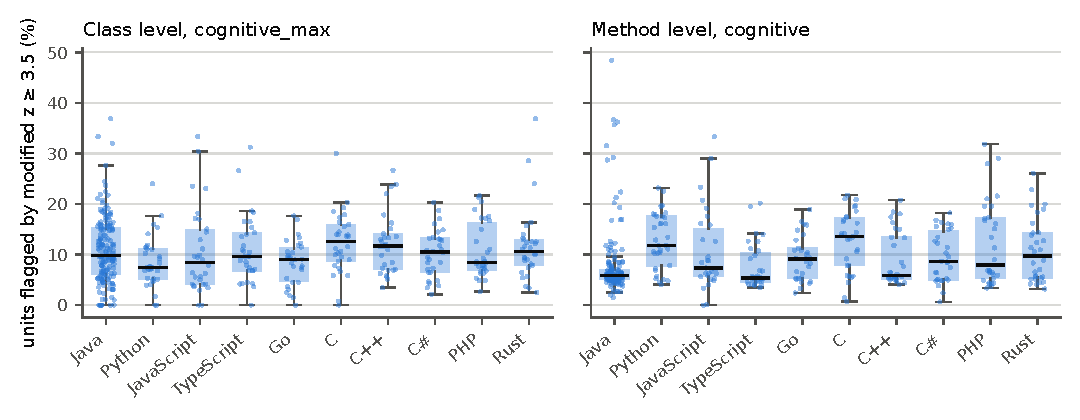
\includegraphics[width=\textwidth]{figures/flag_rates.pdf}
\caption{The share of units the modified z-score at its default flags, per
repository, by language. Every repository of the main run; a box is the
interquartile range, the line the median.}
\label{fig:flagrates}
\end{figure}

\subsection{The primary: PMD GodClass at class level}
\label{sec:primary}

PMD's GodClass is present on \primCarryEx{} explore and \primCarryCo{} confirm
Java repositories, marking \primPosEx{} and \primPosCo{} files; \primMinPosEx{}
and \primMinPosCo{} repositories carry three or more, which is where a
per-repository AUC is read. The median Java repository has \pmdGodsMedian{} PMD
god classes and \pmdGodFreeShare{} have none.

\paragraph{Chosen on explore.} Among the peak and density families, the
per-file maximum of cognitive complexity, \sig{cognitive\_max}, had the highest
macro mean per-repository AUC on the explore half, \primExploreAuc{}, ahead of
\primExploreSecond{} at \primExploreSecondAuc{}; the peak family led, and the
best density signal, \primExploreBestDensity{} at \primExploreBestDensityAuc{},
beat only the weakest peak (Table~\ref{tab:explore}). Its absolute competitor,
the cutoff maximising the pooled MCC on explore, is \sig{cognitive\_max} $\geq
\primCut$.

\begin{table}[t]
\centering
\caption{The explore-half choice of the primary signal: macro mean
per-repository AUC against PMD GodClass over the explore repositories with at
least three god classes, peak and density families, ingredients excluded.}
\label{tab:explore}
\small
\fitwidth{% generated by paper/scripts/tables.py; do not edit
\begin{tabular}{llrr}
\toprule
Signal & Family & Macro mean AUC & $n$ repositories \\
\midrule
\texttt{cognitive\_max} (chosen) & peak & 0.916 & 50 \\
\texttt{nloc\_max} & peak & 0.893 & 50 \\
\texttt{nesting\_max} & peak & 0.888 & 50 \\
\texttt{tokens\_max} & peak & 0.885 & 50 \\
\texttt{hvol\_max} & peak & 0.881 & 50 \\
\texttt{exit\_points\_max} & peak & 0.871 & 50 \\
\texttt{cognitive\_mean} & density & 0.811 & 50 \\
\texttt{params\_max} & peak & 0.804 & 50 \\
\texttt{nesting\_mean} & density & 0.747 & 50 \\
\texttt{nloc\_mean} & density & 0.747 & 50 \\
\texttt{hvol\_mean} & density & 0.742 & 50 \\
\texttt{exit\_points\_mean} & density & 0.737 & 50 \\
\texttt{tokens\_mean} & density & 0.737 & 50 \\
\texttt{params\_mean} & density & 0.621 & 50 \\
\bottomrule
\end{tabular}
}
\end{table}

\paragraph{Read on confirm.} The signal carries the definition. Its macro
per-repository AUC on confirm is \primAucMacro{}, interval \primAucMacroCI{}
over \primAucMacroN{} repositories, clearing the 0.70 floor; within the files
that already pass the WMC $\geq 47$ clause it falls to \primAucGiven{}
\primAucGivenCI{}: much of what the signal separates is the size clause, and
something is left beyond it. The peak is not a sum, but it is not free of size
either. Per repository, \sig{cognitive\_max} correlates with the sum of lines at
Spearman \sizeRhoNlocSum{} \sizeRhoNlocSumCI{} and with the method count at
\sizeRhoNom{} \sizeRhoNomCI{} over the \sizeRhoNomN{} confirm repositories: a
file with more methods has a higher maximum, and the family labelling is read
with that in mind. Figure~\ref{fig:aucbysignal} shows the same
per-repository AUC for every class signal: the size family sits highest, as
size recovering size should, the peak family next, and the density family
lowest and widest.

\begin{figure}[p]
\centering
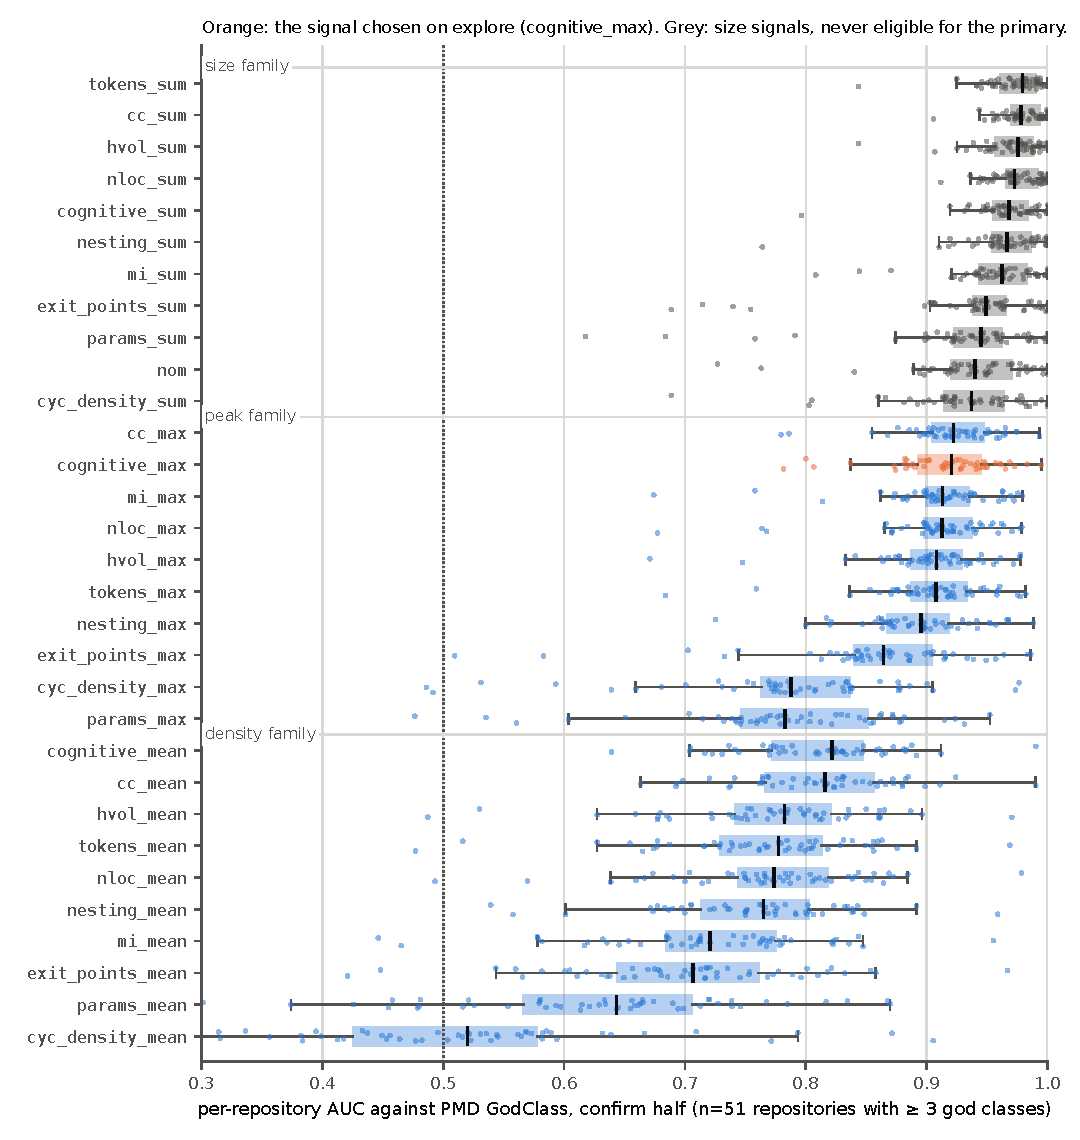
\includegraphics[width=\textwidth]{figures/auc_by_signal.pdf}
\caption{Per-repository AUC of every class-level signal against PMD GodClass on
the confirm half, grouped by family. One point per repository with at least
three god classes; the box is the interquartile range. Size signals are grey
because the plan never allowed one to headline a definition with a size clause.}
\label{fig:aucbysignal}
\end{figure}

The threshold-free comparison goes against the relative view. Pooling every
confirm unit into one ranking, the AUC is \primPooledAucRaw{} on the raw value
and \primPooledAucStd{} on the per-repository modified z, a paired difference of
\primPooledAucDiff{} with interval \primPooledAucDiffCI{}: \emph{\primPooledAucReading}.
Standardising each repository by its own scale costs a little ranking quality
against a definition that is itself an absolute threshold, which is the
direction the tilt predicts.

\begin{table}[t]
\centering
\caption{The primary read-out on the confirm half: the modified z-score at its
literature default against the absolute cutoff tuned on explore, and the tuned
relative cut as a secondary. Macro is one repository, one vote, over the
\primCarryCo{} confirm repositories carrying the definition, god-free ones at
MCC 0; over the \primMacroMccPosN{} with at least one god class, the population
of the decision's macro arm and of the explore level (\primExploreLevel{}), the
two macro MCCs are \primRelMacroMccPos{} and \primAbsMacroMccPos{}. Micro pools
their units. ``FP in god-free'' is the number of flags in the \primNGodFree{}
confirm repositories where PMD marks nothing.}
\label{tab:confirm-primary}
\small
\setlength{\tabcolsep}{4pt}
\fitwidth{% generated by paper/scripts/tables.py; do not edit
\begin{tabular}{lrrrrrr}
\toprule
Rule on \texttt{cognitive\_max} & Macro MCC, god-free at 0 (95\% CI) & Micro MCC & Precision & Recall & Macro FPR & FP in god-free repos \\
\midrule
default: modified $z \geq 3.5$ & 0.278 [0.230, 0.329] & 0.378 & 0.30 & 0.59 & 0.079 & 139/21 \\
tuned absolute cutoff $\geq 22$ & 0.285 [0.229, 0.341] & 0.406 & 0.44 & 0.44 & 0.038 & 19/21 \\
tuned modified $z \geq 2.75$ (secondary) & 0.297 [0.248, 0.346] & 0.380 & 0.27 & 0.67 & 0.102 & 203/21 \\
\bottomrule
\end{tabular}
}
\end{table}

At the operating point (Table~\ref{tab:confirm-primary}) the two rules reach
almost the same macro MCC, \primRelMacroMcc{} for the default modified z against
\primAbsMacroMcc{} for the tuned cutoff, and a lower micro MCC,
\primRelMicroMcc{} against \primAbsMicroMcc{}. The difference is in how they get
there. The relative rule flags \primRelFlagged{} confirm files, recall
\primRelRecall{} at precision \primRelPrecision{}; the absolute cutoff flags
\primAbsFlagged{}, recall \primAbsRecall{} at precision \primAbsPrecision{}. The
relative rule's extra flags are its false positives: a per-repository
false-positive rate of \primRelFprPct{} against \primAbsFprPct{}, and
\primRelFpGodFree{} flags in the \primNGodFree{} god-free repositories against
\primAbsFpGodFree{}, about \primRelMeanFlagsGodFree{} files per such repository
against \primAbsMeanFlagsGodFree{}. Figure~\ref{fig:pooled} shows why. On the
relative axis \primRelRecall{} of PMD's god classes clear 3.5 but so do
\primRelPooledFprPct{} of the other files, because the per-repository tails are
long; on the raw axis the tuned cutoff admits \primAbsPooledFprPct{} of the other
files at the price of recall. The tuned
relative cut, \madz{} replaced by $z \geq \primZCut$, buys recall with more
false positives still and does not change the picture.

\begin{figure}[t]
\centering
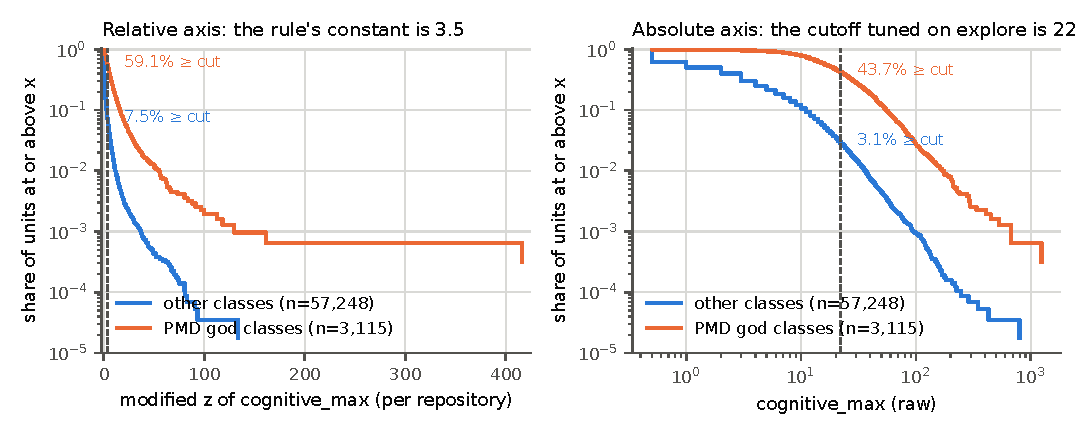
\includegraphics[width=\textwidth]{figures/pooled_distribution.pdf}
\caption{Every Java class unit of the confirm half, pooled: the share of units
at or above $x$, for PMD's god classes and for the rest, on the relative axis
(the per-repository modified z of \sig{cognitive\_max}) and on the absolute
axis (the raw value). Dashed lines are the two rules' cuts.}
\label{fig:pooled}
\end{figure}

\paragraph{The decision.} Table~\ref{tab:decisions} and
Figure~\ref{fig:decisions} give the three paired arms. The MCC margin read is
\primMargin{}, the ceiling, since 0.30 times the explore-half macro MCC
(\primExploreLevel{}) is above it. On the macro MCC arm the paired difference is
\primMacroMcc{}, interval \primMacroMccCI{} over \primMacroMccN{} repositories
with at least one god class: \primMacroMccVerdict. On the micro arm it is
\primMicroMcc{} \primMicroMccCI{} over \primMicroMccN{}: \primMicroMccVerdict.
On the false-positive arm the relative rule is \primMacroFpr{} points worse,
\primMacroFprCI{}: neither below the $+0.05$ margin at its upper bound nor
above it at its lower, so \primMacroFprVerdict. The verdict, the weakest arm, is
\textbf{\primVerdict}. Every point estimate is on the absolute side: both MCC
differences are negative, the pooled ranking is better raw, and the
false-positive rate is higher. Non-inferiority on the MCC arms says only that
the relative rule is not more than 0.10 worse, and 0.10 is about a third of the
MCC level realised. The effective sample is met (\primMinPosCo{} repositories
with three or more positives against 20 needed, \primCarryCo{} carrying the
definition against 40) and the AUC floor is met; the classpath bound is met
too, but out of order (Section~\ref{sec:classpath}), so the verdict is read as
confirmatory with that qualification. Figure~\ref{fig:paired} shows the pairing
repository by repository: the two rules' MCCs lie along the diagonal, and the
relative rule's false-positive rate lies above it in most repositories where
the absolute cutoff flags little.

\begin{table}[t]
\centering
\caption{The pre-registered decision for every definition read: the paired
difference, relative rule at its default minus the absolute cutoff tuned on
explore, with its 95\% repository bootstrap, on each arm. The MCC margin is
$\min(0.10, 0.30 \times$ explore level$)$; the FPR margin is $+0.05$. The
verdict is the weakest arm among those the plan decides on; $\dagger$ marks an
arm reported but not decided on (the human definitions decide on the micro arm
alone).}
\label{tab:decisions}
\scriptsize
\setlength{\tabcolsep}{3pt}
\fitwidth{% generated by paper/scripts/tables.py; do not edit
\begin{tabular}{lcccrl}
\toprule
Definition (signal) & Macro MCC & Micro MCC & Macro FPR & Margin & Verdict \\
\midrule
PMD GodClass & $-$0.009 & $-$0.028 & +0.042 & 0.100 & \textbf{inconclusive} \\
{\scriptsize \texttt{cognitive\_max}, main run} & {\scriptsize [$-$0.057, +0.040] non-inferior} & {\scriptsize [$-$0.068, +0.005] non-inferior} & {\scriptsize [+0.027, +0.056] inconclusive} & & \\[2pt]
PMD NPath $\geq 200$ & $-$0.256 & $-$0.331 & +0.052 & 0.098 & \textbf{inferior} \\
{\scriptsize \texttt{cc}, main run} & {\scriptsize [$-$0.308, $-$0.204] inferior} & {\scriptsize [$-$0.380, $-$0.284] inferior} & {\scriptsize [+0.047, +0.057] inconclusive} & & \\[2pt]
DECOR Blob (approx.) & $-$0.023 & $-$0.032 & $-$0.033 & 0.072 & \textbf{non-inferior} \\
{\scriptsize \texttt{cognitive\_max}, main run} & {\scriptsize [$-$0.055, +0.006] non-inferior} & {\scriptsize [$-$0.063, +0.001] non-inferior} & {\scriptsize [$-$0.058, $-$0.011] superior} & & \\[2pt]
Brain Method (internal) & $-$0.322 & $-$0.172 & +0.087 & 0.066 & \textbf{inferior} \\
{\scriptsize \texttt{cognitive}, main run} & {\scriptsize [$-$0.355, $-$0.290] inferior} & {\scriptsize [$-$0.292, $-$0.095] inferior} & {\scriptsize [+0.078, +0.096] inferior} & & \\[2pt]
PMD GodClass & $-$0.020 & $-$0.098 & +0.007 & 0.100 & \textbf{inconclusive} \\
{\scriptsize \texttt{cognitive\_max}, MLCQ repositories} & {\scriptsize [$-$0.039, $-$0.003] non-inferior} & {\scriptsize [$-$0.151, $-$0.063] inconclusive} & {\scriptsize [$-$0.005, +0.018] non-inferior} & & \\[2pt]
MLCQ Blob (human) & $-$0.284 & $-$0.228 & $-$0.271 & 0.014 & \textbf{inferior} \\
{\scriptsize \texttt{mi\_max}, MLCQ reviewed units} & {\scriptsize [$-$0.389, $-$0.186] inferior$^{\dagger}$} & {\scriptsize [$-$0.324, $-$0.115] inferior} & {\scriptsize [$-$0.321, $-$0.225] superior$^{\dagger}$} & & \\[2pt]
MLCQ Long Method (human) & $-$0.358 & $-$0.362 & +0.032 & 0.100 & \textbf{inferior} \\
{\scriptsize \texttt{mi}, MLCQ reviewed units} & {\scriptsize [$-$0.473, $-$0.242] inferior$^{\dagger}$} & {\scriptsize [$-$0.492, $-$0.242] inferior} & {\scriptsize [+0.000, +0.069] inconclusive$^{\dagger}$} & & \\[2pt]
\bottomrule
\end{tabular}
}
\end{table}

\begin{figure}[t]
\centering
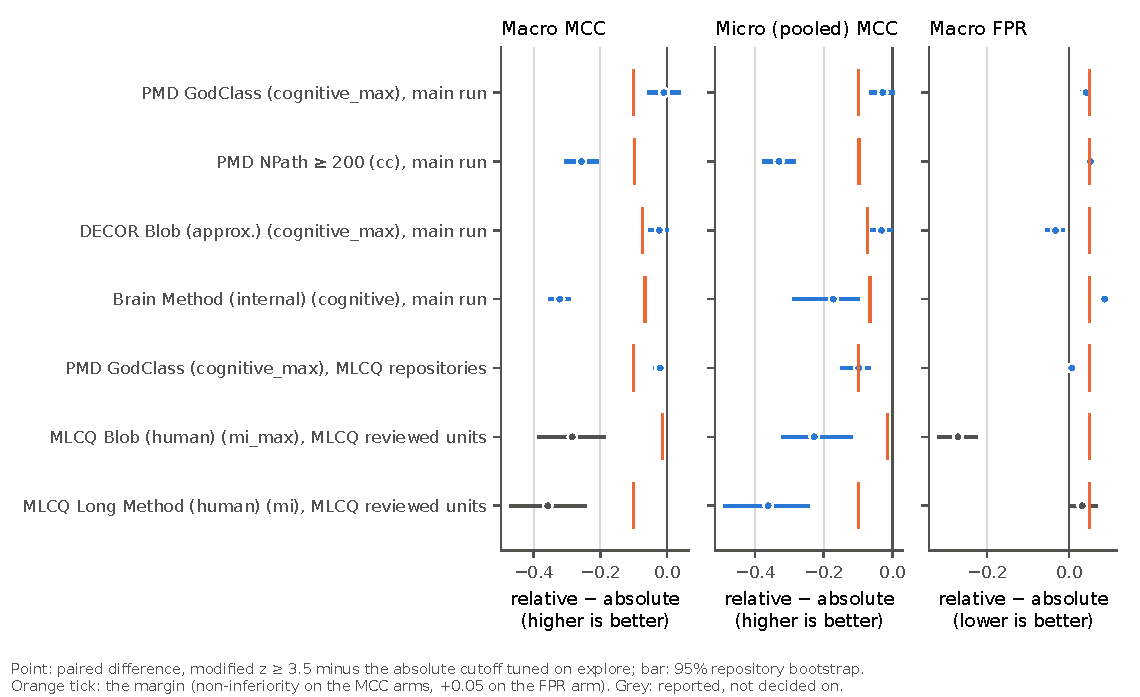
\includegraphics[width=\textwidth]{figures/decisions.pdf}
\caption{The decision arms of Table~\ref{tab:decisions}. On the MCC arms the
margin tick sits at $-m$ and a bar wholly to its right is non-inferior; on the
FPR arm it sits at $+0.05$ and a bar wholly to its left is non-inferior.}
\label{fig:decisions}
\end{figure}

\begin{figure}[t]
\centering
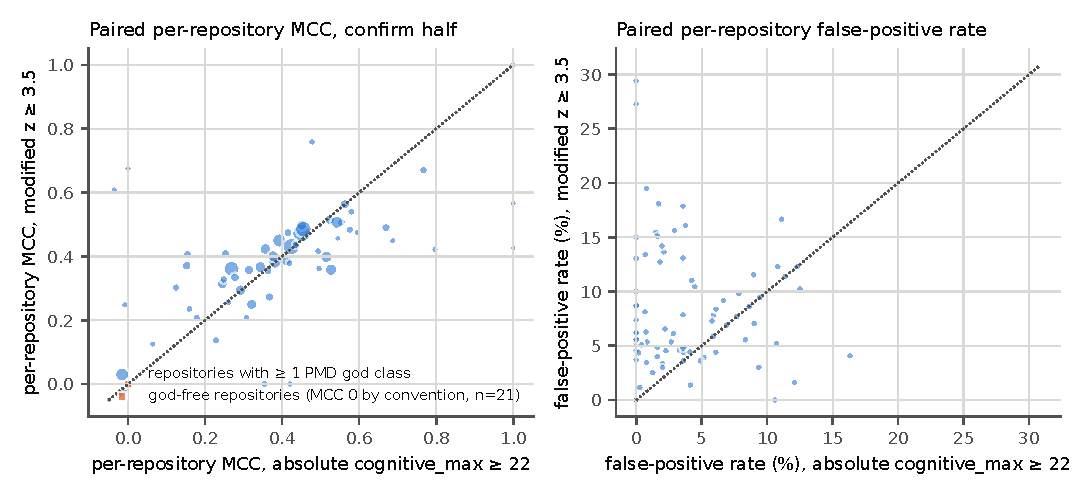
\includegraphics[width=\textwidth]{figures/paired_mcc.pdf}
\caption{The pairing behind the decision: each point is one confirm Java
repository carrying PMD GodClass, with the per-repository MCC (left, point size
by the number of god classes) and false-positive rate (right) of the two rules
on \sig{cognitive\_max}.}
\label{fig:paired}
\end{figure}

\paragraph{Breakdowns.} The result is the same in every slice. The macro AUC is
\primBrTierHighAuc{} in the high tier, \primBrTierMidAuc{} in the mid tier and
\primBrTierLowAuc{} in the low tier; the default rule's macro MCC is
\primBrTierHighMcc{}, \primBrTierMidMcc{} and \primBrTierLowMcc{}. Applications
(\primBrKindApplicationN{} repositories) and libraries (\primBrKindLibraryN{})
give AUCs of \primBrKindApplicationAuc{} and \primBrKindLibraryAuc{}.

\subsection{Secondary definitions}
\label{sec:secondary}

Table~\ref{tab:secondary} summarises the three secondary definitions of the
main run; each has the same read-out as the primary, and their decision arms
are in Table~\ref{tab:decisions}.

\begin{table}[t]
\centering
\caption{The secondary definitions of the main run, chosen on explore and read
on confirm. The pooled AUC difference is standardised minus raw; the micro MCCs
are the default modified z and the explore-tuned absolute cutoff.}
\label{tab:secondary}
\scriptsize
\setlength{\tabcolsep}{4pt}
\fitwidth{% generated by paper/scripts/tables.py; do not edit
\begin{tabular}{llrrrrrr}
\toprule
Definition & Signal & Macro AUC & Pooled AUC std$-$raw & Rel.\ micro MCC & Abs.\ cut & Abs.\ micro MCC & Verdict \\
\midrule
PMD NPath $\geq 200$ & \texttt{cc} & 0.996 [0.994, 0.996] & -0.004 [-0.007, -0.002] & 0.250 & 15 & 0.580 & inferior \\
DECOR Blob (approx.) & \texttt{cognitive\_max} & 0.737 [0.704, 0.770] & +0.025 [-0.023, +0.065] & 0.230 & 12 & 0.261 & non-inferior \\
Brain Method (internal) & \texttt{cognitive} & 0.985 [0.972, 0.995] & -0.003 [-0.010, +0.010] & 0.189 & 38 & 0.361 & inferior \\
\bottomrule
\end{tabular}
}
\end{table}

\paragraph{PMD NPath at method level.} Cyclomatic complexity ranks PMD's NPath
positives almost perfectly, a macro AUC of \npathAucMacro{}, since the two
measures count nearly the same branches. The relative rule is nonetheless
\textbf{\npathVerdict}: it flags \npathRelFlagged{} confirm methods to recover
\npathRelRecall{} of the \npathPosCo{} positives at precision
\npathRelPrecision{}, where the tuned cutoff \sig{cc} $\geq \npathCut$ flags
\npathAbsFlagged{} at precision \npathAbsPrecision{} and recall
\npathAbsRecall{}. The micro MCC difference is \npathMicroMcc{}
\npathMicroMccCI{}. This is the shape diagnostic made concrete: with more than
half of all methods at cyclomatic complexity 1 the scale falls back to the mean
absolute deviation, 3.5 of those deviations is a low bar, and the rule flags a
twentieth of every repository's methods. A cut tuned on the relative axis,
$z \geq \npathZCut$, closes much of the gap, so the failure is the literature
constant on this shape of distribution, not the standardisation.

\paragraph{DECOR Blob (approximate).} The approximate Blob is the one definition on which the
relative rule is \textbf{\decorVerdict}, non-inferior on both MCC arms
(\decorMacroMcc{} \decorMacroMccCI{} and \decorMicroMcc{} \decorMicroMccCI{}) and
superior on false positives (\decorMacroFpr{} \decorMacroFprCI{}). The tuned
cutoff for this definition is a low \sig{cognitive\_max} $\geq \decorCut$,
which flags \decorAbsFprPct{} of non-Blob files per repository, more than the
relative rule's \decorRelFprPct{}; DECOR's Blob is mostly a size and cohesion
definition and the peak signal ranks it at only \decorAucMacro{}. The
threshold-free difference here favours the relative ranking in point estimate
(\decorPooledAucDiff{}) without resolving (\decorPooledAucDiffCI{}).

\paragraph{Brain Method.} The internal composite is recovered by cognitive
complexity at a macro AUC of \brainAucMacro{}, as a conjunction of its
ingredients' cousins should be, and the relative rule is \textbf{\brainVerdict}
on every arm for the NPath reason: \brainRelFlagged{} flags for \brainPosCo{}
positives.

\subsection{Rules and signals compared}

Table~\ref{tab:friedman} ranks the five pre-specified rules by per-repository
MCC and the six pre-specified signals by per-repository AUC against PMD
GodClass, in both runs. Among rules, the modified z-score (mean rank
\friedRankMadZ), Tukey's fence (\friedRankIqr) and the one-sided MAD
(\friedRankDoubleMad), in that order, are within a critical difference of
\friedRulesCD{} of one another and separated from the top percentile
(\friedRankPctTopOne) and the skew-adjusted boxplot (\friedRankAdjBoxplot),
over \friedRulesN{} repositories.
Among signals, the per-file sum of lines ranks first (\friedSigRankNlocSum) and
the method count second (\friedSigRankNom), both size; among the non-size
signals the two peaks, \sig{cc\_max} (\friedSigRankCcMax) and
\sig{cognitive\_max} (\friedSigRankCognitiveMax), are within the critical
difference of \friedSignalsCD{} of each other and well ahead of the two means.
The MLCQ run reproduces both orderings with its larger $N$, and its smaller
critical difference separates the one-sided MAD from the first two rules.

\begin{table}[t]
\centering
\caption{Friedman tests over repositories with the Iman--Davenport correction,
rules by per-repository MCC and signals by per-repository AUC against PMD
GodClass, pre-specified subsets, both runs. Lower mean rank is better; two
methods closer than the Nemenyi critical difference are not separated.}
\label{tab:friedman}
\scriptsize
\fitwidth{% generated by paper/scripts/tables.py; do not edit
\begin{tabular}{lrl}
\toprule
Method & Mean rank & \\
\midrule
\multicolumn{3}{l}{\emph{Main run: rules by per-repository MCC against PMD GodClass on cognitive\_max}} \\
\multicolumn{3}{l}{\quad $N=131$, $k=5$, Iman--Davenport $F=27.1$, $p=1.9\times10^{-20}$, Nemenyi CD$_{0.05}=0.533$, all-tied blocks dropped 39} \\
\quad \texttt{mad\_z} & 2.42 & \\
\quad \texttt{iqr} & 2.50 & \\
\quad \texttt{double\_mad} & 2.67 & \\
\quad \texttt{pct\_top1} & 3.56 & \\
\quad \texttt{adj\_boxplot} & 3.85 & \\
\addlinespace
\multicolumn{3}{l}{\emph{Main run: signals by per-repository AUC against PMD GodClass}} \\
\multicolumn{3}{l}{\quad $N=101$, $k=6$, Iman--Davenport $F=542.1$, $p=2.9\times10^{-199}$, Nemenyi CD$_{0.05}=0.750$, all-tied blocks dropped 0} \\
\quad \texttt{nloc\_sum} & 1.19 & \\
\quad \texttt{nom} & 2.52 & \\
\quad \texttt{cc\_max} & 3.02 & \\
\quad \texttt{cognitive\_max} & 3.36 & \\
\quad \texttt{cc\_mean} & 4.92 & \\
\quad \texttt{mi\_mean} & 5.99 & \\
\addlinespace
\multicolumn{3}{l}{\emph{MLCQ run: rules by per-repository MCC}} \\
\multicolumn{3}{l}{\quad $N=454$, $k=5$, Iman--Davenport $F=221.7$, $p=5.5\times10^{-155}$, Nemenyi CD$_{0.05}=0.286$, all-tied blocks dropped 36} \\
\quad \texttt{mad\_z} & 2.17 & \\
\quad \texttt{iqr} & 2.23 & \\
\quad \texttt{double\_mad} & 2.68 & \\
\quad \texttt{pct\_top1} & 3.80 & \\
\quad \texttt{adj\_boxplot} & 4.12 & \\
\addlinespace
\multicolumn{3}{l}{\emph{MLCQ run: signals by per-repository AUC}} \\
\multicolumn{3}{l}{\quad $N=408$, $k=6$, Iman--Davenport $F=2036.0$, $p<10^{-300}$, Nemenyi CD$_{0.05}=0.373$, all-tied blocks dropped 0} \\
\quad \texttt{nloc\_sum} & 1.09 & \\
\quad \texttt{nom} & 2.66 & \\
\quad \texttt{cc\_max} & 3.10 & \\
\quad \texttt{cognitive\_max} & 3.28 & \\
\quad \texttt{cc\_mean} & 4.96 & \\
\quad \texttt{mi\_mean} & 5.90 & \\
\bottomrule
\end{tabular}
}
\end{table}

\subsection{The classpath validation, out of order}
\label{sec:classpath}

PMD and CK ran without an auxiliary classpath, so the ATFD clause of GodClass
sees only the sources. The plan bounded that under-count by building at least
ten explore-half Java repositories with their own Maven or Gradle wrappers,
re-running PMD with the built classpath over the same file list, and counting
the GodClass verdicts that flip, with a bound of 10\%. It was due before the
confirm half was read and was run after: the candidates were ordered by a seeded
shuffle of every explore Java repository with at least one god class, worked
down in order, \cpTried{} attempted, \cpFailed{} failing to build under any of
four JDKs and \cpSkipped{} skipped (no build, or an Android SDK required), until
\cpRepos{} had a report (Table~\ref{tab:classpath}). \cpFlips{} of \cpUnion{}
verdicts flipped, \cpRate{}, every one a god class gained with the classpath
and \cpMaxFlips{} of them in one repository (\cpMaxFlipsRepo{}). The bound is met, so the under-count is small
and one-sided: the oracle misses some god classes, which can only lower the
recovery measured against it. Because the order of events was wrong, the
confirmatory analysis file records the primary verdict as not confirmatory for
want of the validation, and the re-analysis that applied the bound is a dated
exploratory file; the two agree on every number. The paper reads the verdict as
confirmatory with this deviation declared, and a reader who holds to the
plan's order may read the primary as exploratory.

\begin{table}[t]
\centering
\caption{The classpath validation: ten explore-half Java repositories built with
their own build tool, PMD GodClass verdicts without and with the built
classpath over the same files.}
\label{tab:classpath}
\small
\fitwidth{% generated by paper/scripts/tables.py; do not edit
\begin{tabular}{lrrrrr}
\toprule
Repository & Java files & Classpath entries & GodClass without & with & Flips (lost/gained) \\
\midrule
Anuken/Mindustry & 1152 & 48 & 118 & 141 & 0/23 \\
Berikai/bitwig-theme-editor & 16 & 15 & 2 & 2 & 0/0 \\
appium/java-client & 634 & 33 & 6 & 6 & 0/0 \\
blendi-remade/falcraft & 38 & 111 & 6 & 6 & 0/0 \\
cabaletta/baritone & 376 & 170 & 24 & 25 & 0/1 \\
jenkinsci/jenkins & 1346 & 248 & 65 & 66 & 0/1 \\
jfree/jfreechart & 666 & 10 & 81 & 81 & 0/0 \\
microsoft/playwright-java & 228 & 18 & 14 & 15 & 0/1 \\
openpreserve/jhove & 472 & 85 & 44 & 44 & 0/0 \\
resilience4j/resilience4j & 736 & 135 & 4 & 4 & 0/0 \\
\midrule
Total & & & & & 26 of 390 verdicts (6.7\%) \\
\bottomrule
\end{tabular}
}
\end{table}

\subsection{Replication on MLCQ's population}
\label{sec:mlcq-pmd}

The same plan, read on the \mlcqUsable{} usable MLCQ repositories with their own
explore and confirm halves and PMD's GodClass as the oracle, chooses the same
signal, \mlcqPmdSignal{}, at a macro AUC of \mlcqPmdAucMacro{}
\mlcqPmdAucMacroCI{} over \mlcqPmdAucMacroN{} confirm repositories, and reaches
the same verdict, \textbf{\mlcqPmdVerdict}: the macro MCC arm is
\mlcqPmdMacroMccVerdict{} (\mlcqPmdMacroMcc{} \mlcqPmdMacroMccCI{}), the FPR arm
\mlcqPmdMacroFprVerdict{} (\mlcqPmdMacroFpr{} \mlcqPmdMacroFprCI{}), and the
micro arm \mlcqPmdMicroMccVerdict{} (\mlcqPmdMicroMcc{} \mlcqPmdMicroMccCI{}),
with the margin again at \mlcqPmdMargin{}. The population is older, larger and
more concentrated by owner, the tuned cutoff is lower (\sig{cognitive\_max}
$\geq \mlcqPmdCut$ against \primCut{} in the main run), and the relative rule's
false-positive rate is \mlcqPmdRelFprPct{} against the cutoff's
\mlcqPmdAbsFprPct{}: the same shape of result, with the micro arm reaching
further below the margin than on the sampled population. The three secondaries
replicate too: NPath \mlcqNpathVerdict{} (\mlcqNpathMicroMcc{}
\mlcqNpathMicroMccCI{}), Brain Method \mlcqBrainVerdict{}, and DECOR Blob
\mlcqDecorVerdict{} with the signal \mlcqDecorSignal{} chosen in place of
\sig{cognitive\_max}.

\subsection{Exploratory: the cutoff carried across populations}
\label{sec:transfer}

Every comparison above tunes the absolute cutoff on one population's explore
half and reads it on the same population's confirm half, the best case for a
raw-scale constant. The paper's motivation is that such a constant has to be
re-fitted when the population moves, and the relative rule's claim is that it
does not. The two populations here are seven years and a sampling frame
apart: MLCQ's Java projects at 2019 commits, chosen by its authors, and the
2026 sample. Table~\ref{tab:transfer} reads each confirm half three ways: the
relative rule at its default, the cutoff tuned on that population, and the
cutoff tuned on the other population and carried across unchanged. This
read-out was added after the first draft of the paper was reviewed and is
exploratory.

\begin{table}[t]
\centering
\caption{Exploratory: the absolute cutoff on \sig{cognitive\_max} carried
between populations, against PMD GodClass on each population's confirm half.
Macro MCC is over the repositories with at least one god class, macro FPR over
every repository carrying the definition.}
\label{tab:transfer}
\small
\setlength{\tabcolsep}{4pt}
\fitwidth{% generated by paper/scripts/tables.py; do not edit
\begin{tabular}{llrrrrrr}
\toprule
Read on & Rule & Cut & Micro MCC & Macro MCC & Macro FPR & Precision & Recall \\
\midrule
main run, confirm half & relative, modified $z \geq 3.5$ & -- & 0.378 & 0.371 & 0.079 & 0.30 & 0.59 \\
 & absolute, tuned on this population & 22 & 0.406 & 0.380 & 0.038 & 0.44 & 0.44 \\
 & absolute, tuned on the MLCQ & 17 & 0.421 & 0.401 & 0.063 & 0.37 & 0.56 \\
\addlinespace
MLCQ, confirm half & relative, modified $z \geq 3.5$ & -- & 0.385 & 0.370 & 0.087 & 0.35 & 0.56 \\
 & absolute, tuned on this population & 17 & 0.483 & 0.390 & 0.080 & 0.41 & 0.69 \\
 & absolute, tuned on the main run & 22 & 0.476 & 0.376 & 0.053 & 0.47 & 0.57 \\
\addlinespace
\bottomrule
\end{tabular}
}
\end{table}

The constant transfers almost intact. Tuned on the main run the cutoff is
\sig{cognitive\_max} $\geq \transferMainOwnCut$, on MLCQ $\geq
\transferMlcqOwnCut$. Read on the main run's confirm half, MLCQ's cutoff does
no worse than the main run's own: micro MCC \transferMainAbsOtherMicroMcc{}
against \transferMainAbsOwnMicroMcc{} and macro MCC
\transferMainAbsOtherMacroMcc{} against \transferMainAbsOwnMacroMcc{}, paired
differences of \transferMainOtherMinusOwnMicroMcc{}
\transferMainOtherMinusOwnMicroMccCI{} and \transferMainOtherMinusOwnMacroMcc{}
\transferMainOtherMinusOwnMacroMccCI{}, at a false-positive rate
\transferMainOtherMinusOwnMacroFpr{} higher
\transferMainOtherMinusOwnMacroFprCI{}. Read on MLCQ, the main run's cutoff
costs \transferMlcqOtherMinusOwnMicroMcc{} \transferMlcqOtherMinusOwnMicroMccCI{}
of micro MCC and \transferMlcqOtherMinusOwnMacroMcc{}
\transferMlcqOtherMinusOwnMacroMccCI{} of macro MCC, with fewer false positives
(\transferMlcqOtherMinusOwnMacroFpr{} \transferMlcqOtherMinusOwnMacroFprCI{}).
Against the carried constant the relative rule is behind on the micro arm on
both populations, \transferMainRelMinusOtherMicroMcc{}
\transferMainRelMinusOtherMicroMccCI{} and \transferMlcqRelMinusOtherMicroMcc{}
\transferMlcqRelMinusOtherMicroMccCI{}, level on the macro arm
(\transferMainRelMinusOtherMacroMcc{} \transferMainRelMinusOtherMacroMccCI{};
\transferMlcqRelMinusOtherMacroMcc{} \transferMlcqRelMinusOtherMacroMccCI{}),
and flags more (\transferMainRelMinusOtherMacroFpr{}
\transferMainRelMinusOtherMacroFprCI{}; \transferMlcqRelMinusOtherMacroFpr{}
\transferMlcqRelMinusOtherMacroFprCI{}).

What moves is the optimum per repository, not the pooled one. The cutoff that
maximises a single confirm repository's own MCC runs from
\transferMainOptCutMin{} to \transferMainOptCutMax{} on the main run, quartiles
\transferMainOptCutQOne{}, \transferMainOptCutMedian{} and
\transferMainOptCutQThree{} over the \transferMainOptCutN{} repositories with
three or more god classes, and from \transferMlcqOptCutMin{} to
\transferMlcqOptCutMax{} on MLCQ (quartiles \transferMlcqOptCutQOne{},
\transferMlcqOptCutMedian{}, \transferMlcqOptCutQThree{}). The raw value at
which the relative rule's 3.5 falls in a repository, its implied cutoff, is as
spread: quartiles \transferMainZCutQOne{}, \transferMainZCutMedian{} and
\transferMainZCutQThree{} on the main run. Repositories differ a great deal in
where their god classes sit on the raw axis, and the relative rule follows
that spread; but following it does not recover PMD's verdicts better than one
constant for everyone, because PMD's definition is itself one constant for
everyone. Between these two populations, that constant did not need
re-fitting.

\subsection{Human labels}
\label{sec:human}

\paragraph{Coverage.} Of MLCQ's \mlcqRepos{} repositories, \mlcqRunDone{} were
measured and \mlcqRunFailed{} could not be cloned at their labelled commit, most
of them Eclipse projects that have moved organisation; \mlcqUsable{} cleared the
substance floor. Of the Blob reviews on the measured repositories
\humBlobRevMeasured{} of \humBlobRevLabelled{} land on a measured file
(\humBlobRevRate{}), the rest on files outside the universe (test directories,
generated code), and \humBlobMeasured{} of the \humBlobLabelled{} Blob positives;
for Long Method \humLmRevMeasured{} of \humLmRevLabelled{} reviewed methods
(\humLmRevRate{}) and \humLmMeasured{} of \humLmLabelled{} positives, after
stepping a label that starts on an annotation line forward to the method it
names.

\paragraph{The planned read-out.} For Blob, \humBlobAllReposEx{} explore and
\humBlobAllReposCo{} confirm repositories have at least one reviewed class,
\humBlobAllRevEx{} and \humBlobAllRevCo{} reviewed classes with
\humBlobAllPosEx{} and \humBlobAllPosCo{} positives, but only
\humBlobAllMinPosEx{} and \humBlobAllMinPosCo{} repositories have three or more
positives, so the explore choice rests on nine repositories and the
effective-sample gate (20) is not met. The plan's procedure chose
\humBlobAllSignal{}, the per-file maximum of the maintainability burden, and the
choice exposes a flaw in the plan rather than bad luck. The maintainability
index is bounded and built on logarithms of volume, complexity and lines, so its
upper tail is compressed; a per-repository AUC, the criterion the plan chooses
by, is invariant to that compression, while a modified z of 3.5 on the
compressed axis is out of reach in most repositories. A plan that admits a
bounded composite into a family chosen by AUC will pick it whenever it ranks
well and then read a rule that cannot flag: \madz{} on it flags
\humBlobAllRelFlagged{} of \humBlobAllRevCo{} reviewed classes (recall
\humBlobAllRelRecall{}) against the tuned cutoff's \humBlobAllAbsFlagged{}
(recall \humBlobAllAbsRecall{}, precision \humBlobAllAbsPrecision{}). The micro
MCC difference is \humBlobAllMicroMcc{} \humBlobAllMicroMccCI{}:
\textbf{\humBlobAllVerdict}, \humBlobAllPowered{}, and with the AUC floor not
met (\humBlobAllAucMacro{} \humBlobAllAucMacroCI{}). The margin the plan's
formula gives here is \humBlobAllMargin{}, 0.30 of an explore level of
\humBlobAllExploreLevel{}, below anything the sample could resolve, so this
read-out could never have been non-inferior: the formula degenerates when the
explore level is near zero, a second flaw in the plan.
For Long Method the procedure chose \humLongMethodAllSignal{}, the method-level
maintainability burden, which ranks the reviewers' positives at a macro AUC of
\humLongMethodAllAucMacro{} but again under-flags on the relative axis: micro
MCC \humLongMethodAllRelMicroMcc{} for the default rule against
\humLongMethodAllAbsMicroMcc{} for the cutoff, difference
\humLongMethodAllMicroMcc{} \humLongMethodAllMicroMccCI{},
\textbf{\humLongMethodAllVerdict} and \humLongMethodAllPowered{}
(\humLongMethodAllMinPosCo{} confirm repositories with three or more
positives). Tables~\ref{tab:human-class} and \ref{tab:human-method} give both
read-outs in full, and both decision rows are in Table~\ref{tab:decisions}.
Restricted to the repositories whose reviewed units hold a positive
(Section~\ref{sec:deviations}), the verdicts are unchanged.

\begin{table}[t]
\centering
\caption{The planned human-label read-out for MLCQ's Blob on the confirm half,
every repository with a reviewed class kept, rules fitted on each repository's
whole Java class population and scored on its reviewed classes.}
\label{tab:human-class}
\small
\setlength{\tabcolsep}{4pt}
\fitwidth{% generated by paper/scripts/tables.py; do not edit
\begin{tabular}{lrrrrrr}
\toprule
Rule on \texttt{mi\_max} & Macro MCC (95\% CI) & Micro MCC & Precision & Recall & Macro FPR & FP in god-free repos \\
\midrule
default: modified $z \geq 3.5$ & 0.005 [-0.001, 0.015] & 0.024 & 0.20 & 0.01 & 0.006 & 2/138 \\
tuned absolute cutoff $\geq 52.93$ & 0.091 [0.056, 0.130] & 0.252 & 0.21 & 0.68 & 0.277 & 102/138 \\
tuned modified $z \geq 1.03$ (secondary) & 0.070 [0.035, 0.110] & 0.229 & 0.24 & 0.47 & 0.167 & 54/138 \\
\bottomrule
\end{tabular}
}
\end{table}

\begin{table}[t]
\centering
\caption{The same for MLCQ's Long Method at method level.}
\label{tab:human-method}
\small
\setlength{\tabcolsep}{4pt}
\fitwidth{% generated by paper/scripts/tables.py; do not edit
\begin{tabular}{lrrrrrr}
\toprule
Rule on \texttt{mi} & Macro MCC (95\% CI) & Micro MCC & Precision & Recall & Macro FPR & FP in god-free repos \\
\midrule
default: modified $z \geq 3.5$ & 0.148 [0.104, 0.194] & 0.423 & 0.51 & 0.47 & 0.071 & 26/123 \\
tuned absolute cutoff $\geq 50.63$ & 0.276 [0.218, 0.336] & 0.785 & 0.73 & 0.91 & 0.039 & 12/123 \\
tuned modified $z \geq 2.40$ (secondary) & 0.203 [0.154, 0.255] & 0.506 & 0.42 & 0.80 & 0.168 & 58/123 \\
\bottomrule
\end{tabular}
}
\end{table}

\paragraph{Every candidate, beside the chosen one.} Because the choice rested on
nine repositories, Tables~\ref{tab:human-cand-class} and
\ref{tab:human-cand-method} give the confirm read-out of every candidate signal.
They are exploratory: the plan reads the chosen signal, and the best of twenty
is upward-biased. For Blob no signal does well. The pooled standardised AUC of
the best peak signals sits between 0.73 and 0.77, the default relative rule's micro
MCC peaks at about 0.22 (\sig{tokens\_max}) and the tuned cutoffs at about
0.26, with precision around a quarter at either operating point. For Long
Method the two structure signals, \sig{cc} and \sig{cognitive}, give the
relative rule at its default a micro MCC of about 0.60 to 0.62 against about
0.67 to 0.68 for their tuned cutoffs, so on those signals the default rule is
close to a cutoff tuned with hindsight, while on \sig{mi} it is not.

\paragraph{Tools and rules against the reviewers.} The exploratory comparison
that the main result called for asks two things of the reviewed units: how well
each fixed definition agrees with the reviewers at all, and whether the classes
the relative rule flags that PMD does not, its false positives in the main run,
are classes people call Blob. Nothing here is tuned on MLCQ: the signal, the
rule and the cutoff are the main run's (\primSignal{} with \madz{} and the
cutoff \primCut{}; \sig{cc} with the cutoff \npathCut{} at method level), so
every usable repository with a reviewed unit is used, the confirm half alone
being reported in the data as a sensitivity. Table~\ref{tab:agreement} and
Figure~\ref{fig:agreement} give the answers.

\begin{table}[t]
\centering
\caption{Exploratory: each fixed definition and the main run's two rules as a
predictor of the reviewers' verdict, over the reviewed units of every usable
MLCQ repository, with a 95\% repository bootstrap on the MCC.}
\label{tab:agreement}
\small
\setlength{\tabcolsep}{4pt}
\fitwidth{% generated by paper/scripts/tables.py; do not edit
\begin{tabular}{lrrrrl}
\toprule
Predictor & Flagged & Precision & Recall & MCC & 95\% CI \\
\midrule
\multicolumn{6}{l}{\emph{Blob}: 390 repositories, 1{,}827 reviewed units, 204 reviewer positives (base rate 11.2\%)} \\
\quad PMD GodClass & 236 & 0.31 & 0.36 & +0.242 & [+0.186, +0.301] \\
\quad DECOR Blob (approx.) & 335 & 0.24 & 0.40 & +0.196 & [+0.142, +0.256] \\
\quad WMC $\geq 47$ & 398 & 0.25 & 0.48 & +0.226 & [+0.171, +0.283] \\
\quad relative: modified $z \geq 3.5$ on \texttt{cognitive\_max} & 326 & 0.25 & 0.40 & +0.202 & [+0.153, +0.254] \\
\quad absolute: \texttt{cognitive\_max} $\geq 22$ & 242 & 0.29 & 0.34 & +0.220 & [+0.162, +0.284] \\
\addlinespace
\multicolumn{6}{l}{\emph{Long Method}: 392 repositories, 1{,}988 reviewed units, 220 reviewer positives (base rate 11.1\%)} \\
\quad PMD NPath $\geq 200$ & 28 & 0.93 & 0.12 & +0.312 & [+0.244, +0.371] \\
\quad CC $\geq 14$ & 47 & 0.96 & 0.20 & +0.420 & [+0.353, +0.485] \\
\quad cognitive $\geq 15$ & 102 & 0.87 & 0.40 & +0.565 & [+0.497, +0.629] \\
\quad NLOC $\geq 50$ & 68 & 0.91 & 0.28 & +0.481 & [+0.412, +0.542] \\
\quad Brain Method (internal) & 4 & 1.00 & 0.02 & +0.127 & [+0.060, +0.189] \\
\quad relative: modified $z \geq 3.5$ on \texttt{cc} & 205 & 0.65 & 0.60 & +0.582 & [+0.517, +0.641] \\
\quad absolute: \texttt{cc} $\geq 15$ & 45 & 0.98 & 0.20 & +0.421 & [+0.354, +0.485] \\
\addlinespace
\bottomrule
\end{tabular}
}
\end{table}

\begin{figure}[t]
\centering
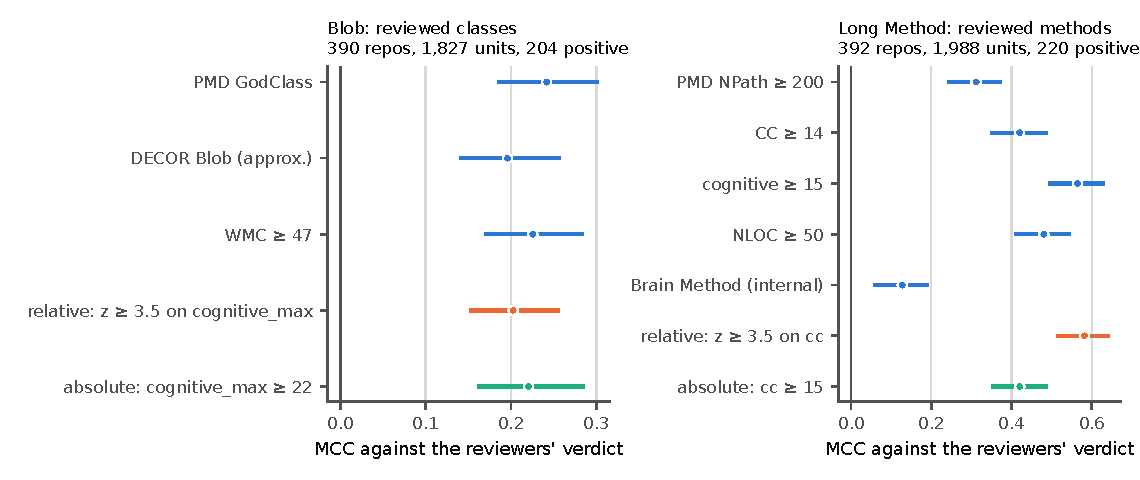
\includegraphics[width=\textwidth]{figures/human_agreement.pdf}
\caption{The MCC of each definition and rule against MLCQ's reviewers, with its
95\% repository bootstrap, on the reviewed classes (Blob) and methods (Long
Method). Orange: the relative rule; aqua: the absolute cutoff tuned on the main
run's explore half.}
\label{fig:agreement}
\end{figure}

On Blob, every detector is weak and none is separated from the others. PMD's
GodClass reaches an MCC of \agrBlobPmdGodclassMcc{} \agrBlobPmdGodclassMccCI{}
against the \agrBlobPos{} reviewer positives among \agrBlobUnits{} reviewed
classes, WMC $\geq 47$ alone \agrBlobWmcFourSevenMcc{}, the relative rule
\agrBlobRelMcc{} \agrBlobRelMccCI{} and the absolute cutoff \agrBlobAbsMcc{}
\agrBlobAbsMccCI{}, each flagging between a quarter and a third of what it
flags correctly. The reviewers' Blob rate is \agrBlobGrpToolRate{} among the
classes PMD flags, \agrBlobGrpRelNotToolRate{} among the
\agrBlobGrpRelNotToolN{} classes the relative rule flags and PMD does not, and
\agrBlobGrpNeitherRelNorToolRate{} among the classes neither flags: the rule's
extra flags are called Blob more than twice as often as unflagged classes, the
paired difference \agrBlobRelExtraDiff{} \agrBlobRelExtraDiffCI{}, and the
absolute cutoff's extra flags more often still (\agrBlobAbsExtraDiff{}
\agrBlobAbsExtraDiffCI{}). Four in five of the classes the relative rule adds to
PMD's list are not Blobs to the reviewers either. No paired difference between
the relative rule and a fixed definition is resolved: against PMD GodClass
\agrBlobRelMinusPmdGodclass{} \agrBlobRelMinusPmdGodclassCI{}, against the
tuned cutoff \agrBlobRelMinusAbs{} \agrBlobRelMinusAbsCI{}.

On Long Method the picture is different and sharper. The fixed thresholds are
precise and recall little: PMD's NPath flags \agrLmPmdMethodNpathTwoZeroZeroFlagged{}
of the \agrLmUnits{} reviewed methods at precision
\agrLmPmdMethodNpathTwoZeroZeroPrecision{} and recall
\agrLmPmdMethodNpathTwoZeroZeroRecall{} (MCC \agrLmPmdMethodNpathTwoZeroZeroMcc{}),
CC $\geq 14$ recall \agrLmCcOneFourRecall{} (MCC \agrLmCcOneFourMcc{}), fifty
lines \agrLmLocFiveZeroRecall{} (\agrLmLocFiveZeroMcc{}), cognitive $\geq 15$
\agrLmCognitiveOneFiveRecall{} (\agrLmCognitiveOneFiveMcc{}
\agrLmCognitiveOneFiveMccCI{}), and the tuned cutoff \sig{cc} $\geq \npathCut$
recall \agrLmAbsRecall{} (\agrLmAbsMcc{}). The relative rule on \sig{cc} trades
precision for recall, \agrLmRelPrecision{} and \agrLmRelRecall{}, and has the
highest MCC point estimate of the detectors tried, \agrLmRelMcc{}
\agrLmRelMccCI{}. Paired over repositories on the same units, its lead is
resolved over PMD's NPath (\agrLmRelMinusPmdMethodNpathTwoZeroZero{}
\agrLmRelMinusPmdMethodNpathTwoZeroZeroCI{}), CC $\geq 14$
(\agrLmRelMinusCcOneFour{} \agrLmRelMinusCcOneFourCI{}), fifty lines
(\agrLmRelMinusLocFiveZero{} \agrLmRelMinusLocFiveZeroCI{}) and the tuned
cutoff (\agrLmRelMinusAbs{} \agrLmRelMinusAbsCI{}), and not over cognitive
$\geq 15$ (\agrLmRelMinusCognitiveOneFive{}
\agrLmRelMinusCognitiveOneFiveCI{}): against the strongest fixed threshold the
two sit at different operating points with no difference resolved. Its extra
flags over PMD's NPath are called Long Method \agrLmGrpRelNotToolRate{} of the
time against \agrLmGrpNeitherRelNorToolRate{} for unflagged methods. Read with
Table~\ref{tab:human-cand-method}, where the same signal at the same default
reaches a micro MCC of about 0.62 on the confirm half against about 0.67 for a
cutoff tuned on MLCQ's own explore half, the relative rule on cyclomatic
complexity is close to the best a tuned constant does against the reviewers,
ahead of every literature constant but one and level with that one, while the
plan's own procedure, choosing by per-repository AUC on thirteen repositories,
picked the one candidate on which it fails.

\subsection{Exploratory: what the false positives are}
\label{sec:fp}

The relative rule's extra flags against PMD are the cost the decision turned
on, and the reading offered for them in Section~\ref{sec:disc}, that
complexity concentration finds complex leaves as well as god classes, is a
claim about what those files are. Two read-outs test it, both added after the
first draft of the paper was reviewed and both exploratory. The first
characterises every one of them by the tool definitions' own component
clauses. Over the \fpUnits{} Java class units of the \fpRepos{} confirm
repositories carrying PMD GodClass, Table~\ref{tab:fp-breakdown} splits the
units into those the rule flags and PMD marks (\fpTpN{}), those the rule flags
and PMD does not (\fpFpN{}), those PMD marks and the rule misses (\fpFnN{}) and
the rest, and gives for each the share that passes PMD's size clause (the
harness's WMC $\geq 47$, which tracks PMD's own WMC closely but not exactly),
the share a coupling component marks (CK's CBO $\geq 14$ or PMD's
CouplingBetweenObjects), the share a cohesion component marks (CK's TCC $<
1/3$ or LCOM* $\geq 0.8$), and the medians of the signal, the lines and the
method count.

\begin{table}[t]
\centering
\caption{Exploratory: every Java class unit of the confirm repositories
carrying PMD GodClass, grouped by the relative rule's flag and PMD's verdict,
with the share each group's units meet of PMD's size clause and of the coupling
and cohesion components, and the group medians. The last row is the
explore-tuned absolute cutoff's own extra flags.}
\label{tab:fp-breakdown}
\scriptsize
\setlength{\tabcolsep}{3pt}
\fitwidth{% generated by paper/scripts/tables.py; do not edit
\begin{tabular}{lrrrrrrrr}
\toprule
Group & Units & Repos. & WMC $\geq 47$ & Coupled & Low cohesion & Median \texttt{cognitive\_max} & Median lines & Median methods \\
\midrule
flagged by the rule and marked by PMD & 1{,}841 & 56 & 96.8\% & 74.3\% & 86.5\% & 29 & 415 & 32 \\
flagged by the rule, not marked by PMD & 4{,}288 & 78 & 24.1\% & 38.5\% & 84.1\% & 17 & 113 & 9 \\
marked by PMD, not flagged by the rule & 1{,}274 & 50 & 91.9\% & 66.8\% & 91.0\% & 11 & 272 & 32 \\
neither & 52{,}960 & 84 & 2.5\% & 8.2\% & 78.4\% & 1 & 27 & 5 \\
flagged by the absolute cutoff, not marked by PMD & 1{,}753 & 64 & 40.6\% & 45.1\% & 83.1\% & 30 & 165 & 10 \\
\bottomrule
\end{tabular}
}
\end{table}

The extra flags are not god classes by size. Only \fpFpWmcFourSevenPct{} of
them pass the size clause (\fpFpWmcFourSevenPctCI{}), against
\fpTpWmcFourSevenPct{} of the classes PMD marks; their median file has
\fpFpMedianNom{} methods and \fpFpMedianNloc{} lines against \fpTpMedianNom{}
and \fpTpMedianNloc{}, and a maximum cognitive complexity of \fpFpMedianRaw{}
against \fpTpMedianRaw{}. A coupling component marks \fpFpCoupledPct{} of them
(\fpFpCoupledPctCI{}), against \fpTpCoupledPct{} of PMD's god classes and
\fpNeitherCoupledPct{} of unflagged classes. The cohesion components mark most
classes of every group and separate nothing. The absolute cutoff's own extra
flags (\fpAbsFpN{}) are larger and more often coupled than the relative rule's,
\fpAbsFpWmcFourSevenPct{} passing the size clause and \fpAbsFpCoupledPct{}
coupled, which is the other face of its lower false-positive rate: at a raw
cutoff the extra flags are big classes that missed on data access or cohesion,
at a relative cut they are small classes with one complex method. The typical
extra flag of the relative rule is therefore a file of about ten methods whose
most complex method is an outlier for its repository: a concentration of
complexity in a small unit, which is what the rule was built to find, and not,
by PMD's own components, a class that gathers responsibilities, which is what
PMD's definition is built to find. Whether it is one to a reader is the second
read-out's question.

The second read-out reads the source. A seeded sample of \fpSampleFp{} of the
rule's extra flags and \fpSampleTp{} of the classes it flags that PMD also
marks, at most \fpSamplePerRepo{} per repository, was fetched at its pinned
commit and read blind to PMD's verdict under a fixed protocol: four yes-or-no
questions, whether the most complex method implements one algorithm over the
class's own inputs, whether the class has one responsibility, whether it works
mostly on other objects' data, and whether its complexity is one dispatch
table, with a fixed mapping from the answers to four categories (leaf,
gatherer, table, other), written before any file was opened. Reading
conventions that settle what the questions leave open (what counts as one
algorithm, as cohesion, as foreign data and as a dispatch table) were added on
21 October 2026, after the author had read 13 units and before any model
reading; they change no question or mapping row, and the author re-read those
13 units under them. The scripts that
draw the sample and apply the mapping are in the repository; every reader's
answers, with the units they refer to, are in the ancillary data, as are the
recorded sessions of the language-model reader, which a script ran blind, each
session seeing only the protocol and its batch of files.

\begin{table}[t]
\centering
\caption{Exploratory: the blinded reading of \fpSampleFp{} of the relative
rule's extra flags and \fpSampleTp{} of its flags that PMD also marks, by the
author on a seeded subset and by a language model on every unit, each unit's
category given by the protocol's fixed mapping of the four answers. Leaf: one
algorithm, one responsibility, own data. Gatherer: more than one
responsibility, or mostly other objects' data. Table: one dispatch table.}
\label{tab:fp-readings}
\small
\fitwidth{% generated by paper/scripts/tables.py; do not edit
\begin{tabular}{llrrrrr}
\toprule
Reader & Group & $n$ & Leaf & Gatherer & Table & Other \\
\midrule
author & flagged by the rule, not marked by PMD & 20 & 5 (25\%) & 15 (75\%) & 0 (0\%) & 0 (0\%) \\
author & flagged by the rule and marked by PMD & 20 & 1 (5\%) & 19 (95\%) & 0 (0\%) & 0 (0\%) \\
model & flagged by the rule, not marked by PMD & 100 & 66 (66\%) & 17 (17\%) & 5 (5\%) & 12 (12\%) \\
model & flagged by the rule and marked by PMD & 100 & 58 (58\%) & 30 (30\%) & 2 (2\%) & 10 (10\%) \\
\multicolumn{7}{l}{agreement author with model: 21 of 40 units, Cohen's $\kappa = 0.20$} \\
\bottomrule
\end{tabular}
}
\end{table}

Table~\ref{tab:fp-readings} gives the reading. The author read a seeded subset
of \fpReadAuthorFpN{} extra flags and \fpReadAuthorTpN{} of PMD's god classes,
before the model read and before either reading was scored; the model, Claude
Fable 5.1 through the Claude Code command line (version 2.1.307), read all
\fpSampleN{} in ten sessions of twenty files. The two readers do not agree on
what the files are. To the author \fpReadAuthorFpGathererPct{} of the extra
flags are gatherers and \fpReadAuthorFpLeafPct{} leaves, against
\fpReadAuthorTpGathererPct{} and \fpReadAuthorTpLeafPct{} of PMD's god
classes; to the model \fpReadModelFpLeafPct{} of the extra flags are leaves
and \fpReadModelFpGathererPct{} gatherers, against \fpReadModelTpLeafPct{} and
\fpReadModelTpGathererPct{}. Each reader puts more leaves among the extra
flags than among PMD's god classes and more gatherers among PMD's, the
direction the component breakdown predicts, but each reads the two groups
more alike than apart, and on the \fpKappaAuthorModelN{} units both read they
give the same category to \fpKappaAuthorModelAgree{}, Cohen's $\kappa$ of
\fpKappaAuthorModel{}. The disagreement sits in one question. On whether the
most complex method implements one algorithm the readers say yes at much the
same rate in both groups (the author for \fpReadAuthorFpQOneYesPct{} of the
extra flags and \fpReadAuthorTpQOneYesPct{} of PMD's god classes, the model
for \fpReadModelFpQOneYesPct{} and \fpReadModelTpQOneYesPct{}), so the
complexity the rule finds is, to both readers, mostly an algorithm's, god
class or not. On whether the class has one responsibility they part: the
author says yes for \fpReadAuthorFpQTwoYesPct{} of the extra flags and
\fpReadAuthorTpQTwoYesPct{} of PMD's god classes, the model for
\fpReadModelFpQTwoYesPct{} and \fpReadModelTpQTwoYesPct{}, and their $\kappa$
on that question is \fpKappaAuthorModelQTwo{}, chance agreement. The one
question they answer alike is whether the class works mostly on other objects'
data ($\kappa$ \fpKappaAuthorModelQThree{}), and on it both separate the
groups the same way, the author widely and the model narrowly: yes for
\fpReadAuthorFpQThreeYesPct{} of the extra flags against
\fpReadAuthorTpQThreeYesPct{} of PMD's god classes to the author, and for
\fpReadModelFpQThreeYesPct{} against \fpReadModelTpQThreeYesPct{} to the
model. Dispatch tables are few to both. The reading therefore does not
establish that the extra flags are leaves. Whether a class has one
responsibility is a judgement two readers made differently on the same files
under the same written conventions, and the mapping turns on it; what the two
readers could judge alike, and what separated the extra flags from PMD's god
classes to both, is whether the class works on other objects' data, which is
the coupling question the follow-on study measures rather than reads.

\subsection{Exploratory: the whole matrix}

Table~\ref{tab:exploratory} (Appendix~\ref{app:tables}) gives, for every definition in the registry, the
signal with the highest macro AUC over all repositories and the signal-and-rule
cell with the highest macro MCC, in the main run. It is a search over 31
signals, seven rules and two dozen definitions, upward-biased and reported as
such. Three patterns are worth stating. Every self definition is recovered by
its own signal at AUC 1, as it must be. Every PMD size and coupling component
is best recovered by a size signal. And where the best signal is an ingredient
it is marked, so that a reader does not take \sig{cc\_sum} recovering PMD's
GodClass, which contains WMC, as a finding.

\section{Deviations from the plan}
\label{sec:deviations}

One thing did not go to plan, and one part of the analysis was computed outside
the harness. Each is stated with its effect.

\paragraph{The classpath validation ran after confirm was read.} Described in
Section~\ref{sec:classpath}. The validation touched explore repositories only,
nothing in the analysis changed, and the bound was met; the order was wrong,
and the confirmatory file records the primary as not confirmatory for that
reason. Effect on the numbers: none. Effect on status: the reader's call.

\paragraph{The human read-out is computed by the paper's scripts.} The
harness's analysis of record covers the tool definitions. It writes its
definition registry before the first repository is measured and reads its
secondaries from that registry, which for the MLCQ run holds no human
definition, so the planned human read-out is performed by this paper's
scripts, with the harness's statistics module and the plan's constants, on the
reviewed units reduced from the per-unit sidecar under the registry written at
the end of the run. The extraction is checked against the harness's own
analysis file on the main run, where every number it reproduces agrees to nine
decimals. The read-out was first computed on 2026-10-20 and last regenerated
on \humComputedUtc{}, with every number unchanged; nothing about the procedure
was chosen after seeing it, and the plan it follows is the one tagged before
the run. Two readings are reported. The plan keeps a god-free
repository, so the paper keeps every repository with a reviewed unit at that
level, its reviewed units being negatives the reviewers did look at; that is
the plan-faithful reading and the one the paper quotes. Restricted to the
\humBlobPosReposCo{} confirm repositories with a Blob positive, the Blob
micro-MCC difference is \humBlobPosMicroMcc{} \humBlobPosMicroMccCI{}, and on
the \humLongMethodPosReposCo{} repositories with a Long Method positive the
difference is \humLongMethodPosMicroMcc{} \humLongMethodPosMicroMccCI{}: the
same verdicts. Both readings are in the ancillary data. The exploratory
agreement of Section~\ref{sec:human} is likewise the paper's, on the reviewed
units. An earlier version of it in the harness, written before the MLCQ run,
scored every Java class of each repository (218{,}896 units over 136
repositories, with MCCs near 0.03 because the unreviewed classes were taken as
negatives); it is superseded by the paper's, with the same questions,
decisions and readings, and its output is kept in the ancillary data as a
record.

\paragraph{Added after review.} Four read-outs were added after the first
draft of this paper was reviewed, none pre-registered and each labelled
exploratory where it appears: the paired differences in the agreement
comparison (Section~\ref{sec:human}, computed \agrComputedUtc{}), the
cross-population transfer (Section~\ref{sec:transfer}, \transferComputedUtc{}),
the size correlations of the primary signal (Section~\ref{sec:primary}) and
the characterisation and reading of the false positives
(Section~\ref{sec:fp}, \fpComputedUtc{}). Effect on the pre-registered
numbers: none. Effect on the reading: the transfer read-out weakens the
motivation, and the paper says so.

\section{Discussion}
\label{sec:disc}

\paragraph{What inconclusive means here.} The scale-free rule did not beat
the tuned cutoff on anything measured. It recovers PMD's god classes from a
signal that is not a size sum at a per-repository AUC above 0.9, and within
the pre-registered margin it matches a cutoff tuned with hindsight on
recovery, on a second population and in every tier. But every point estimate
is on the cutoff's side: the pooled ranking is better raw than standardised,
the rule flags about twice as many non-god classes, and the cutoff carried
from the other population beats it too. The verdict is inconclusive because
the plan made the false-positive arm decide and that arm neither cleared its
margin nor fell below it; non-inferiority on the MCC arms, at a margin a third
of the level, says only that the rule is not much worse. A rule that flagged
half as much would have passed the plan; it would also have recalled less.

\paragraph{What the false positives are.} The relative rule's extra flags are
small classes carrying one complex method. Three in four fail PMD's size
clause, their median file has \fpFpMedianNom{} methods, and a coupling
component marks \fpFpCoupledPct{} of them against \fpTpCoupledPct{} of PMD's
god classes; against MLCQ's reviewers one in six of them is a Blob, more than
twice the rate among unflagged classes and less than the rate among PMD's
flags. Reading the source did not settle whether they are leaves. Both readers
found the complexity to be an algorithm's in about seven files of ten, god
class or not; on whether the class around it has one responsibility the author
and the model disagreed at chance, the author calling three in four of the
extra flags gatherers and the model two in three leaves; and the one judgement
the two shared, whether the class works on other objects' data, was the one
that separated the extra flags from PMD's god classes to both. The reading
that fits is that complexity concentration locates where a codebase's
complexity has gathered, and that whether the place is a god unit is legible
neither in the complexity nor, reliably, in a reader's sense of responsibility,
but in what the unit does with other objects' data. A leaf that holds the
complexity of the algorithm it computes, a parser, a solver, a state machine,
is an outlier for its repository and is exactly where that complexity belongs.
Complexity alone cannot tell it from a class that gathers responsibilities,
every definition in this study that does so adds a coupling clause to do it,
and the coupling question was the one the two readers could answer alike.
That is what the follow-on study takes up: whether a method's or class's
coupling divergence, what it hands on to the rest of the system against what it
receives, separates a complex leaf from a god unit among the units complexity
alone flags. Its plan was registered before the human-label numbers here
existed and records what of this study it had seen.

\paragraph{Method level is a different problem.} At method level the rule
fails against every tool definition and, on the plan's chosen signal, against
the reviewers, for one reason: most methods have the lowest possible value,
the robust scale collapses to a mean deviation, and 3.5 of it is a low bar.
Yet on the two structure signals the default rule reaches a micro MCC within
0.08 of a cutoff tuned on MLCQ's own explore half against the reviewers' Long
Method verdicts, ahead of every literature constant but one and level with
that one. The constant is the
problem, not the standardisation, and a scale-free rule for methods needs a
constant fitted to the shape of method-level distributions, which this study
did not register and does not claim.

\paragraph{Humans against tools.} The weakest numbers in this paper are the
ones every detector shares. No tool definition and no rule agrees with MLCQ's
reviewers on Blob beyond an MCC of about 0.24, in line with what Schumacher et
al.\ found for inter-developer agreement itself \cite{schumacher2010} and far
below the 0.51 that classifiers trained on the labels reach \cite{mlcq2023}.
On Long Method the fixed thresholds are precise and recall little, which is
what a constant chosen to be safe does, and the relative rule recalls more at a
price in precision. Whether a team wants the first or the second is a choice
about cost, not a fact about the rule.

\paragraph{The drift argument.} The motivation was that raw-scale constants
stand in for a reader's budget, that the budget moves as the population of
code moves, and that AI agents writing and maintaining code may be moving it
now. Nothing here measures readers or budgets, and agreement with a definition
cannot show its constant drifting. What the transfer read-out shows is
narrower and goes the other way: between MLCQ's 2019 projects and the 2026
sample, a cutoff tuned on one population lost almost nothing on the other, and
the relative rule, which needs no re-fitting, did not beat the constant that
was never re-fitted. On these two populations there was no drift to be free
of. Both are populations of code written largely by people. The one comparison
found that sets LLM-generated code beside human-written code on a fixed task
saw concentration rise with the share of LLM involvement, and saw the
threshold-based smell detectors miss it \cite{zhang2026llm}; that is one
assignment of small projects, and this study's sample holds no such contrast. The cost of the relative rule, a doubling of false positives at a precision
of \primRelPrecision{} against \primAbsPrecision{}, is large to a user of a
detector, and on this evidence it buys nothing. Whether a population written
largely by agents moves the constant is a question this study's sample, drawn
in 2026 from repositories of every age, does not isolate; a comparison of
repositories by agent adoption, of the kind He et al.\ made for complexity
\cite{he2026cursor}, would.

\paragraph{Conservation, revisited.} The companion study's finding that
complexity is conserved and placed was the context in which concentration,
rather than level, came to be the question. The results here do not test
conservation, and conservation was never a premise of the rule; what they test
is whether the place where a system's complexity has gathered is the god unit
the definitions in use mark. It is, for where the complexity sits, and it is
not, for what the complexity is. A conserved quantity has to sit somewhere,
and some of the places it sits are the right ones.

\section{Threats to validity}
\label{sec:threats}

\paragraph{Construct.} Every tool definition is itself an absolute threshold
and itself imperfect, so against the tools this measures agreement between
detectors on terms that favour the absolute competitor. The approximate DECOR
Blob omits the association clause and uses the study's own cohesion cut; the
Brain Method is internal and omits the NOAV clause; cognitive complexity,
Halstead volume, the maintainability index and nesting are lexical estimators,
calibrated against PMD. Each signal is a single indicator of a construct with
several facets; reading the rule across ten of them, in
families fixed in advance, stands in for a measurement model of complexity and
is not one. The class-level unit is the file. The human labels are
the only oracle without a constant inside it, and they are absolute judgements
by readers who did not see the repository; their reviewers agreed with one
another only moderately.

\paragraph{Internal.} PMD and CK ran without a classpath; the validation bounds
the effect at \cpRate{} of verdicts on ten repositories and was run out of
order. Test code is excluded by directory conventions that can miss or
over-match; generated files and files over 1~MB leave the universe and are
counted. The class-level unit is the file, and \javaFilesMultiPct{} of Java
files hold more than one class, so a nested class's verdict and its methods'
complexity are credited to the file that holds it. The relative rules are fitted with zeros included, which makes the
zero-heavy method-level signals fall back to a mean-deviation scale; the scale
kind is recorded and reported. The human read-out was computed by the paper's
scripts, checked against the harness on the main run, and rests on
\humBlobAllMinPosEx{} (Blob) and \humLongMethodAllMinPosEx{} (Long Method)
repositories for its signal choice and on \humBlobAllAucMacroN{} and
\humLongMethodAllAucMacroN{} for its per-repository AUC.

\paragraph{External.} GitHub repositories of 200 stars or more, ten languages,
one commit each, drawn with equal allocation across three popularity tiers, so
pooled numbers are unweighted over strata and not population estimates. Every
composite definition is Java-only, so the recovery result is a Java,
class-level result; the other nine languages supply the flag-rate and
scale-kind diagnostics and no recovery of an external definition. The MLCQ
population is MLCQ's choice, half of it Apache, at 2019 commits, and its
intervals overstate its independence; its reviewed units were drawn at random
and then enriched by re-review, so the base rate among them is MLCQ's, and
agreement with its reviewers is read at that rate. The sampler is a separate tool but the author's own; it takes no
input from the study beyond its criteria, and its draw is reproducible from
the published derivation. Re-running it reproduces the method, not necessarily
the list; the published sample files, pinned to commits, are the record.

\paragraph{Conclusion validity.} The matrix is a large search; its single best
cells are upward-biased, which is why one primary, one decision rule and one
read of the confirm half were fixed in advance and why the all-candidate tables
of the human read-out are labelled exploratory. The within-repository AUC is the
same under both views and is never read as evidence for scale-freeness. The
human-label gate was not met, so no human-label result here is confirmatory,
and the one favourable human-label number, the relative rule on cyclomatic
complexity against Long Method, is an exploratory comparison, read with a
paired test, that a reader should expect to shrink on replication. The
cross-population transfer, the component breakdown of the false positives and
the reading of a sample of them were added after the first draft of this paper
was reviewed; none was pre-registered and each is labelled exploratory. The
reading has two readers, one of them the author and the other a language
model whose answers are not a human's, who agree on the category at a $\kappa$
of \fpKappaAuthorModel{}; the author read \fpKappaAuthorModelN{} units and the
per-question shares are descriptive, with no interval put on them.

\section{Reproducibility and data availability}
\label{sec:repro}

Every number in this paper is produced by a script from the harness's output.
The harness's two confirmatory analysis files, one per run, and the dated
exploratory re-analysis are included with the paper as ancillary data, with
their digests as committed, together with the sample files the repositories
were drawn from, the frozen explore/confirm assignments, the per-repository
summary tables and definition registries the harness writes, the converted MLCQ
labels and their summary, the classpath reports and build log, the paper's own
reductions of the per-unit data for the human read-out and the agreement
comparison, every reader's answers on the false-positive sample with the
model reader's recorded sessions, and the harness's superseded agreement
output. The raw per-unit
data (several gigabytes) is not included; it regenerates by running the
harness on the published sample files, which pin every repository to its
commit, and the ancillary README names the public code repositories of the
harness, the sampler, the companion study and the follow-on study, with the
command behind every table, figure and inline number.

\section{Conclusion}

A unit whose complexity is a robust outlier for its own codebase is, more often
than not, a class that PMD calls a god class, in every tier, in both
applications and libraries, and on two populations. Read as the plan required,
against a cutoff tuned with hindsight, the scale-free rule at its literature
default is behind on every point estimate, within the pre-registered margin on
recovery and worse on false positives, and the verdict is inconclusive.
Carried between the two populations, the tuned cutoff lost almost nothing, so
on these populations, both of code written largely by people, the re-fitting
the rule saves was not needed. At method
level the literature constant is wrong for the shape of the distribution and
the rule is inferior. Against human reviewers the planned read-out is
underpowered and inferior on the signals its procedure chose, while an
exploratory comparison finds every detector weak on Blob and the relative rule
on cyclomatic complexity level with the best fixed threshold on Long Method and
ahead of the rest.

The result that carries forward is the shape of the errors. Concentration
finds where the complexity is. Some of those places are god units, and some
are small classes doing the work they were written to do, and a complexity
measure cannot tell the two apart because the difference is not in the
complexity. Two readers of the source could not tell them apart by eye either,
except on one question, whether the class works on other objects' data. The
difference is in what the unit does with the data it holds, which is a
coupling question, and the next study asks it.

\section*{Competing interests}

The author created and maintains OfficeFloor, a framework whose design rests on
taking data off the control flow, and the construct the follow-on study tests,
coupling divergence, comes from that line of work. This study compares no
frameworks and its sample excludes the author's own ecosystem, but the reading
in Section~\ref{sec:disc}, that the false positives call for a coupling measure,
is the reading the author's interest favours, and a reader should weigh it as
such. The author was also one of the two readers of the false-positive sample;
that reading was blind to PMD's verdict, made under a protocol committed
before it, and is reported beside the model's with their disagreement. The
sampler that drew the repositories is the author's tool as well. The companion
study on conservation, which motivates this one, is the author's as well. Against the interest: the plan, the seed and the decision rule
were fixed before the data existed, the verdict that resulted is inconclusive
rather than favourable, every deviation is reported with its effect,
and a replication needs no cooperation from the author.

\section*{Funding}

This work received no external funding and was carried out and paid for by the
author.

\appendix
\section{Definitions, rules and exploratory tables}
\label{app:tables}

\begin{table}[p]
\centering
\caption{The definitions this paper reads, from the registry written with the
run. Kind: a composite is a multi-clause textbook definition, a tool measure is
one none of the study's signals computes, a self definition restates one signal
as a threshold, a calibration definition is PMD's own implementation of one of
the study's signals, a component is one clause of a definition. Origin: who
computed the label. A signal built from a definition's base measures may never
headline it.}
\label{tab:registry}
\scriptsize
\setlength{\tabcolsep}{4pt}
\fitwidth{% generated by paper/scripts/tables.py; do not edit
\begin{tabular}{llllll}
\toprule
Definition & Level & Kind & Origin & Constant & Base measures \\
\midrule
\texttt{decor\_blob} & class & composite & composed & NMD+NAD >= 20; LCOM* >= 0.8 & \texttt{nom} \\
\texttt{pmd\_GodClass} & class & composite & tool & PMD defaults & \texttt{cc} \\
\texttt{brain\_method} & method & composite & internal & NLOC >= 50 and CC >= 14 and nesting >= 5 & \texttt{cc}, \texttt{nesting}, \texttt{nloc} \\
\texttt{pmd\_method\_NPath200} & method & tool & tool & reportLevel 200 & -- \\
\texttt{wmc47} & class & self & internal & WMC >= 47 & \texttt{cc} \\
\texttt{cc14} & method & self & internal & CC >= 14 & \texttt{cc} \\
\texttt{cognitive15} & method & self & internal & cognitive >= 15 & \texttt{cognitive} \\
\texttt{loc50} & method & self & internal & NLOC >= 50 & \texttt{nloc} \\
\texttt{nesting5} & method & self & internal & nesting >= 5 & \texttt{nesting} \\
\texttt{params5} & method & self & internal & params >= 5 & \texttt{params} \\
\texttt{pmd\_method\_CC10} & method & calibration & tool & methodReportLevel 10 & \texttt{cc} \\
\texttt{pmd\_method\_Cognitive15} & method & calibration & tool & reportLevel 15 & \texttt{cognitive} \\
\texttt{pmd\_method\_Ncss60} & method & calibration & tool & methodReportLevel 60 & \texttt{nloc} \\
\texttt{ck\_CBOhigh} & class & component & tool & CBO >= 14 & -- \\
\texttt{ck\_LCOM} & class & component & tool & LCOM* >= 0.8 & -- \\
\texttt{ck\_LargeClass} & class & component & tool & NMD+NAD >= 20 & \texttt{nom} \\
\texttt{ck\_TCClow} & class & component & tool & TCC < 1/3 with >= 2 methods & -- \\
\texttt{pmd\_CouplingBetweenObjects} & class & component & tool & threshold 20 unique referenced types & -- \\
\texttt{pmd\_ExcessiveClassLength} & class & component & tool & minimum 1000 lines & \texttt{nloc} \\
\texttt{pmd\_ExcessiveImports} & class & component & tool & minimum 30 & -- \\
\texttt{pmd\_ExcessivePublicCount} & class & component & tool & minimum 45 & \texttt{nom} \\
\texttt{pmd\_NcssCount} & class & component & tool & classReportLevel 1500 & \texttt{nloc} \\
\texttt{pmd\_TooManyFields} & class & component & tool & maxfields 15 & -- \\
\texttt{pmd\_TooManyMethods} & class & component & tool & maxmethods 10 & \texttt{nom} \\
\bottomrule
\end{tabular}
}
\end{table}

\begin{table}[p]
\centering
\caption{The relative outlier rules and their standardised-axis constants, as
recorded with the run. The modified z-score is the pre-registered primary; the
classic z-score is a parametric control; the extreme-value rule's default
$p = 1/n$ is a deliberately strict floor.}
\label{tab:rules}
\scriptsize
\setlength{\tabcolsep}{4pt}
\fitwidth{% generated by paper/scripts/tables.py; do not edit
\begin{tabular}{llll}
\toprule
Rule & Family & Flag when & Constant \\
\midrule
\texttt{mad\_z} & modified z-score (Iglewicz and Hoaglin) & $z \geq 3.5$ on $0.6745\,(x-\tilde{x})/\mathrm{MAD}$ & {"cut": 3.5} \\
\texttt{double\_mad} & one-sided (upper) MAD & $z \geq 3.5$, scale from the upper half & {"cut": 3.5} \\
\texttt{iqr} & Tukey's fence & $x > Q_3 + 1.5\,\mathrm{IQR}$ & {"k": 1.5} \\
\texttt{adj\_boxplot} & skew-adjusted boxplot (Hubert and Vandervieren) & $x > Q_3 + 1.5\,e^{3\,\mathrm{MC}}\,\mathrm{IQR}$ & {"k": 1.5, "c\_upper": 3, "c\_lower": 4} \\
\texttt{evt\_pot} & peaks over threshold, GPD tail & fitted tail survival $< 1/n$ above $q_{0.90}$ & {"p": "1/n", "q": 0.9} \\
\texttt{pct\_top1} & top percentile & $x \geq q_{0.99}$ and above the minimum & {"q": 0.99} \\
\texttt{zscore} & classic z-score (parametric control) & $(x-\bar{x})/s \geq 3$ & {"k": 3.0} \\
\bottomrule
\end{tabular}
}
\end{table}

\begin{table}[p]
\centering
\caption{Exploratory: every candidate class signal on the confirm reviewed
classes of MLCQ's Blob, pooled standardised AUC, the default modified z-score's
micro MCC, precision and recall, and the explore-tuned absolute cutoff with its
micro MCC.}
\label{tab:human-cand-class}
\scriptsize
\fitwidth{% generated by paper/scripts/tables.py; do not edit
\begin{tabular}{llrrrrrr}
\toprule
Signal & Family & Pooled AUC (std.) & \multicolumn{3}{c}{modified $z \geq 3.5$} & \multicolumn{2}{c}{absolute, tuned on explore} \\
 & & & micro MCC & precision & recall & cut & micro MCC \\
\midrule
\texttt{hvol\_max} & peak & 0.769 & 0.196 & 0.24 & 0.37 & 1589.96 & 0.257 \\
\texttt{tokens\_max} & peak & 0.767 & 0.219 & 0.28 & 0.34 & 269 & 0.264 \\
\texttt{mi\_max} (chosen) & peak & 0.765 & 0.024 & 0.20 & 0.01 & 52.93 & 0.252 \\
\texttt{nloc\_max} & peak & 0.761 & 0.186 & 0.25 & 0.31 & 27 & 0.246 \\
\texttt{cc\_max} & peak & 0.753 & 0.212 & 0.27 & 0.34 & 6 & 0.265 \\
\texttt{cognitive\_max} & peak & 0.730 & 0.155 & 0.21 & 0.34 & 7 & 0.244 \\
\texttt{hvol\_mean} & density & 0.716 & 0.121 & 0.22 & 0.20 & 331.188 & 0.238 \\
\texttt{cc\_mean} & density & 0.714 & 0.129 & 0.24 & 0.18 & 2.1154 & 0.236 \\
\texttt{nloc\_mean} & density & 0.712 & 0.089 & 0.20 & 0.13 & 8.8 & 0.223 \\
\texttt{tokens\_mean} & density & 0.711 & 0.119 & 0.23 & 0.17 & 56 & 0.231 \\
\texttt{nesting\_max} & peak & 0.708 & 0.047 & 0.21 & 0.03 & 3 & 0.174 \\
\texttt{exit\_points\_max} & peak & 0.705 & 0.143 & 0.25 & 0.20 & 3 & 0.237 \\
\texttt{cognitive\_mean} & density & 0.698 & 0.137 & 0.22 & 0.24 & 1.6 & 0.211 \\
\texttt{mi\_mean} & density & 0.683 & $-$0.018 & 0.06 & 0.01 & 32.9073 & 0.196 \\
\texttt{nesting\_mean} & density & 0.662 & 0.027 & 0.14 & 0.06 & 0.6857 & 0.150 \\
\texttt{params\_max} & peak & 0.647 & $-$0.017 & 0.07 & 0.02 & 3 & 0.161 \\
\texttt{exit\_points\_mean} & density & 0.645 & 0.088 & 0.25 & 0.08 & 1.0526 & 0.156 \\
\texttt{cyc\_density\_max} & peak & 0.640 & 0.039 & 0.13 & 0.18 & 0.3636 & 0.126 \\
\texttt{params\_mean} & density & 0.558 & 0.109 & 0.30 & 0.08 & 1.0333 & 0.061 \\
\texttt{cyc\_density\_mean} & density & 0.430 & $-$0.023 & 0.06 & 0.01 & 0.1144 & $-$0.007 \\
\bottomrule
\end{tabular}
}
\end{table}

\begin{table}[p]
\centering
\caption{The same for the method-level candidates on MLCQ's Long Method.}
\label{tab:human-cand-method}
\scriptsize
\fitwidth{% generated by paper/scripts/tables.py; do not edit
\begin{tabular}{llrrrrrr}
\toprule
Signal & Family & Pooled AUC (std.) & \multicolumn{3}{c}{modified $z \geq 3.5$} & \multicolumn{2}{c}{absolute, tuned on explore} \\
 & & & micro MCC & precision & recall & cut & micro MCC \\
\midrule
\texttt{cognitive} & structure & 0.933 & 0.601 & 0.68 & 0.61 & 9 & 0.681 \\
\texttt{cc} & structure & 0.922 & 0.617 & 0.69 & 0.64 & 6 & 0.674 \\
\texttt{mi} (chosen) & density & 0.917 & 0.423 & 0.51 & 0.47 & 50.63 & 0.785 \\
\texttt{nesting} & structure & 0.874 & 0.441 & 0.55 & 0.46 & 2 & 0.500 \\
\texttt{exit\_points} & structure & 0.686 & 0.268 & 0.56 & 0.18 & 5 & 0.262 \\
\texttt{params} & density & 0.632 & 0.031 & 0.22 & 0.02 & 4 & 0.066 \\
\texttt{cyc\_density} & density & 0.412 & $-$0.040 & 0.04 & 0.01 & 0.7442 & 0.002 \\
\bottomrule
\end{tabular}
}
\end{table}

\begin{table}[p]
\centering
\caption{Exploratory, main run: the best signal by macro AUC and the best
signal-and-rule cell by macro MCC for every definition in the registry.
$^{*}$ marks a signal that is an ingredient of the definition. Best-of-many is
upward-biased.}
\label{tab:exploratory}
\scriptsize
\setlength{\tabcolsep}{3pt}
\fitwidth{% generated by paper/scripts/tables.py; do not edit
\begin{tabular}{llllrlr}
\toprule
Level & Definition & Kind & Best signal (AUC) & & Best cell (macro MCC) & \\
\midrule
class & \texttt{ck\_CBOhigh} & component & \texttt{tokens\_sum} & 0.905 & \texttt{hvol\_sum} / \texttt{mad\_z} & 0.458 \\
class & \texttt{ck\_LCOM} & component & \texttt{cyc\_density\_sum} & 0.803 & \texttt{nom} / \texttt{mad\_z} & 0.385 \\
class & \texttt{ck\_LargeClass} & component & \texttt{nom}$^{*}$ & 0.948 & \texttt{nom} / \texttt{iqr} & 0.546 \\
class & \texttt{ck\_TCClow} & component & \texttt{nom} & 0.933 & \texttt{cyc\_density\_sum} / \texttt{mad\_z} & 0.142 \\
class & \texttt{decor\_blob} & composite & \texttt{nom}$^{*}$ & 0.946 & \texttt{nom} / \texttt{iqr} & 0.509 \\
class & \texttt{pmd\_CouplingBetweenObjects} & component & \texttt{tokens\_sum} & 0.968 & \texttt{nloc\_sum} / \texttt{iqr} & 0.394 \\
class & \texttt{pmd\_ExcessiveImports} & component & \texttt{hvol\_sum} & 0.952 & \texttt{hvol\_sum} / \texttt{iqr} & 0.343 \\
class & \texttt{pmd\_ExcessivePublicCount} & component & \texttt{cyc\_density\_sum} & 0.927 & \texttt{nom} / \texttt{pct\_top1} & 0.301 \\
class & \texttt{pmd\_GodClass} & composite & \texttt{cc\_sum}$^{*}$ & 0.978 & \texttt{cc\_sum} / \texttt{mad\_z} & 0.475 \\
class & \texttt{pmd\_NcssCount} & component & \texttt{tokens\_sum} & 0.953 & \texttt{cc\_sum} / \texttt{evt\_pot} & 0.108 \\
class & \texttt{pmd\_TooManyFields} & component & \texttt{nloc\_sum} & 0.893 & \texttt{nom} / \texttt{zscore} & 0.242 \\
class & \texttt{pmd\_TooManyMethods} & component & \texttt{mi\_sum} & 0.965 & \texttt{mi\_sum} / \texttt{iqr} & 0.536 \\
class & \texttt{wmc47} & self & \texttt{cc\_sum}$^{*}$ & 1.000 & \texttt{cc\_sum} / \texttt{mad\_z} & 0.641 \\
method & \texttt{brain\_method} & composite & \texttt{cc}$^{*}$ & 0.993 & \texttt{nesting} / \texttt{zscore} & 0.293 \\
method & \texttt{cc14} & self & \texttt{cc}$^{*}$ & 1.000 & \texttt{cc} / \texttt{zscore} & 0.595 \\
method & \texttt{cognitive15} & self & \texttt{cognitive}$^{*}$ & 1.000 & \texttt{cognitive} / \texttt{double\_mad} & 0.642 \\
method & \texttt{loc50} & self & \texttt{nloc}$^{*}$ & 1.000 & \texttt{nloc} / \texttt{zscore} & 0.593 \\
method & \texttt{nesting5} & self & \texttt{nesting}$^{*}$ & 1.000 & \texttt{nesting} / \texttt{zscore} & 0.506 \\
method & \texttt{params5} & self & \texttt{params}$^{*}$ & 1.000 & \texttt{params} / \texttt{zscore} & 0.622 \\
method & \texttt{pmd\_method\_CC10} & calibration & \texttt{cc}$^{*}$ & 0.997 & \texttt{cc} / \texttt{zscore} & 0.600 \\
method & \texttt{pmd\_method\_Cognitive15} & calibration & \texttt{cognitive}$^{*}$ & 0.999 & \texttt{cognitive} / \texttt{zscore} & 0.616 \\
method & \texttt{pmd\_method\_NPath200} & tool & \texttt{cc} & 0.996 & \texttt{cc} / \texttt{pct\_top1} & 0.394 \\
method & \texttt{pmd\_method\_Ncss60} & calibration & \texttt{mi}$^{*}$ & 0.999 & \texttt{mi} / \texttt{zscore} & 0.380 \\
\bottomrule
\end{tabular}
}
\end{table}

\begin{thebibliography}{99}

\bibitem{alves2010} T.~L. Alves, C.~Ypma and J.~Visser,
  ``Deriving metric thresholds from benchmark data,''
  in \emph{Proc. IEEE International Conference on Software Maintenance (ICSM)},
  pp.~1--10, 2010.

\bibitem{cktool} M.~Aniche,
  ``Java code metrics calculator (CK),'' 2015. Version 0.7.0.

\bibitem{arif2026} H.~Arif, M.~Kuutila and P.~Ralph,
  ``Assessing the construct validity of object-oriented, class-level code
  quality metrics,''
  in \emph{Proc. ACM/IEEE International Symposium on Empirical Software
  Engineering and Measurement (ESEM)}, 2026; arXiv:2609.20411.

\bibitem{baxter2006} G.~Baxter, M.~Frean, J.~Noble, M.~Rickerby, H.~Smith,
  M.~Visser, H.~Melton and E.~Tempero,
  ``Understanding the shape of Java software,''
  in \emph{Proc. 21st ACM SIGPLAN Conference on Object-Oriented Programming,
  Systems, Languages, and Applications (OOPSLA)}, pp.~397--412, 2006.

\bibitem{brys2004} G.~Brys, M.~Hubert and A.~Struyf,
  ``A robust measure of skewness,''
  \emph{Journal of Computational and Graphical Statistics}, vol.~13, no.~4,
  pp.~996--1017, 2004.

\bibitem{campbell2018} G.~A. Campbell,
  ``Cognitive Complexity: a new way of measuring understandability,''
  SonarSource white paper, 2018.

\bibitem{chicco2020} D.~Chicco and G.~Jurman,
  ``The advantages of the Matthews correlation coefficient (MCC) over F1 score
  and accuracy in binary classification evaluation,''
  \emph{BMC Genomics}, vol.~21, 6, 2020.

\bibitem{ck1994} S.~R. Chidamber and C.~F. Kemerer,
  ``A Metrics Suite for Object Oriented Design,''
  \emph{IEEE Transactions on Software Engineering}, vol.~20, no.~6,
  pp.~476--493, 1994.

\bibitem{davison1997} A.~C. Davison and D.~V. Hinkley,
  \emph{Bootstrap Methods and Their Application}. Cambridge University Press,
  1997.

\bibitem{demsar2006} J.~Dem\v{s}ar,
  ``Statistical Comparisons of Classifiers over Multiple Data Sets,''
  \emph{Journal of Machine Learning Research}, vol.~7, pp.~1--30, 2006.

\bibitem{dinucci2018} D.~Di~Nucci, F.~Palomba, D.~A. Tamburri, A.~Serebrenik and
  A.~De~Lucia,
  ``Detecting code smells using machine learning techniques: Are we there yet?''
  in \emph{Proc. IEEE 25th International Conference on Software Analysis,
  Evolution and Reengineering (SANER)}, pp.~612--621, 2018.

\bibitem{elemam2001} K.~El~Emam, S.~Benlarbi, N.~Goel and S.~N. Rai,
  ``The confounding effect of class size on the validity of object-oriented
  metrics,''
  \emph{IEEE Transactions on Software Engineering}, vol.~27, no.~7,
  pp.~630--650, 2001.

\bibitem{ferreira2012} K.~A.~M. Ferreira, M.~A.~S. Bigonha, R.~S. Bigonha,
  L.~F.~O. Mendes and H.~C. Almeida,
  ``Identifying thresholds for object-oriented software metrics,''
  \emph{Journal of Systems and Software}, vol.~85, no.~2, pp.~244--257, 2012.

\bibitem{fontana2016} F.~Arcelli Fontana, M.~V. M\"antyl\"a, M.~Zanoni and
  A.~Marino,
  ``Comparing and experimenting machine learning techniques for code smell
  detection,''
  \emph{Empirical Software Engineering}, vol.~21, no.~3, pp.~1143--1191, 2016.

\bibitem{fowler1999} M.~Fowler,
  \emph{Refactoring: Improving the Design of Existing Code}. Addison-Wesley,
  1999.

\bibitem{halstead1977} M.~H. Halstead,
  \emph{Elements of Software Science}. Elsevier, 1977.

\bibitem{he2026cursor} H.~He, C.~Miller, S.~Agarwal, C.~K\"astner and
  B.~Vasilescu,
  ``Speed at the cost of quality: How Cursor AI increases short-term velocity
  and long-term complexity in open-source projects,''
  in \emph{Proc. 23rd International Conference on Mining Software Repositories
  (MSR)}, 2026; arXiv:2511.04427.

\bibitem{hubert2008} M.~Hubert and E.~Vandervieren,
  ``An adjusted boxplot for skewed distributions,''
  \emph{Computational Statistics \& Data Analysis}, vol.~52, no.~12,
  pp.~5186--5201, 2008.

\bibitem{iglewicz1993} B.~Iglewicz and D.~C. Hoaglin,
  \emph{How to Detect and Handle Outliers}. ASQC Quality Press, 1993.

\bibitem{lanza2006} M.~Lanza and R.~Marinescu,
  \emph{Object-Oriented Metrics in Practice}. Springer, 2006.

\bibitem{mcCabe1976} T.~J. McCabe,
  ``A Complexity Measure,''
  \emph{IEEE Transactions on Software Engineering}, vol.~SE-2, no.~4,
  pp.~308--320, 1976.

\bibitem{mlcq2020} L.~Madeyski and T.~Lewowski,
  ``MLCQ: Industry-relevant code smell data set,''
  in \emph{Proc. 24th International Conference on Evaluation and Assessment in
  Software Engineering (EASE)}, pp.~342--347, 2020. Data set version 1.1,
  Zenodo record 3666840.

\bibitem{mlcq2023} L.~Madeyski and T.~Lewowski,
  ``Detecting code smells using industry-relevant data,''
  \emph{Information and Software Technology}, vol.~155, 107112, 2023.

\bibitem{marinescu2004} R.~Marinescu,
  ``Detection strategies: metrics-based rules for detecting design flaws,''
  in \emph{Proc. 20th IEEE International Conference on Software Maintenance
  (ICSM)}, pp.~350--359, 2004.

\bibitem{moha2010} N.~Moha, Y.-G. Gu\'eh\'eneuc, L.~Duchien and A.-F. Le~Meur,
  ``DECOR: A Method for the Specification and Detection of Code and Design
  Smells,''
  \emph{IEEE Transactions on Software Engineering}, vol.~36, no.~1, pp.~20--36,
  2010.

\bibitem{nejmeh1988} B.~A. Nejmeh,
  ``NPATH: a measure of execution path complexity and its applications,''
  \emph{Communications of the ACM}, vol.~31, no.~2, pp.~188--200, 1988.

\bibitem{nosek2018} B.~A. Nosek, C.~R. Ebersole, A.~C. DeHaven and D.~T. Mellor,
  ``The preregistration revolution,''
  \emph{Proceedings of the National Academy of Sciences}, vol.~115, no.~11,
  pp.~2600--2606, 2018.

\bibitem{oliveira2014} P.~Oliveira, M.~T. Valente and F.~P. Lima,
  ``Extracting relative thresholds for source code metrics,''
  in \emph{Proc. IEEE Conference on Software Maintenance, Reengineering and
  Reverse Engineering (CSMR-WCRE)}, pp.~254--263, 2014.

\bibitem{oman1992} P.~Oman and J.~Hagemeister,
  ``Metrics for Assessing a Software System's Maintainability,''
  in \emph{Proc. Conference on Software Maintenance (ICSM)}, pp.~337--344, 1992.

\bibitem{landfill2015} F.~Palomba, D.~Di~Nucci, M.~Tufano, G.~Bavota,
  R.~Oliveto, D.~Poshyvanyk and A.~De~Lucia,
  ``Landfill: An open dataset of code smells with public evaluation,''
  in \emph{Proc. 12th Working Conference on Mining Software Repositories (MSR)},
  pp.~482--485, 2015.

\bibitem{pickands1975} J.~Pickands III,
  ``Statistical inference using extreme order statistics,''
  \emph{The Annals of Statistics}, vol.~3, no.~1, pp.~119--131, 1975.

\bibitem{riel1996} A.~J. Riel,
  \emph{Object-Oriented Design Heuristics}. Addison-Wesley, 1996.

\bibitem{conserved} D.~Sagenschneider,
  ``Conserved amount, negotiable placement. Prompting perturbs one architecture,
  an AI reviewer both,'' 2026. \url{https://doi.org/10.5281/zenodo.23190619}

\bibitem{schumacher2010} J.~Schumacher, N.~Zazworka, F.~Shull, C.~Seaman and
  M.~Shaw,
  ``Building empirical support for automated code smell detection,''
  in \emph{Proc. ACM-IEEE International Symposium on Empirical Software
  Engineering and Measurement (ESEM)}, article 8, 2010.

\bibitem{serebrenik2010} A.~Serebrenik and M.~van~den Brand,
  ``Theil index for aggregation of software metrics values,''
  in \emph{Proc. IEEE International Conference on Software Maintenance (ICSM)},
  pp.~1--9, 2010.

\bibitem{tempero2026} E.~Tempero and P.~Ralph,
  ``Making software metrics useful,''
  \emph{IEEE Computer}, in press, 2026, doi:10.1109/MC.2026.3666634;
  arXiv:2603.16012.

\bibitem{tukey1977} J.~W. Tukey,
  \emph{Exploratory Data Analysis}. Addison-Wesley, 1977.

\bibitem{vasa2009} R.~Vasa, M.~Lumpe, P.~Branch and O.~Nierstrasz,
  ``Comparative Analysis of Evolving Software Systems Using the Gini
  Coefficient,'' in \emph{Proc. IEEE International Conference on Software
  Maintenance (ICSM)}, pp.~179--188, 2009.

\bibitem{lizard} T.~Yin,
  ``Lizard: a simple code complexity analyser,'' version 1.23.0.

\bibitem{zhang2026llm} Z.~Zhang, E.~Wen and E.~Tempero,
  ``Can LLMs produce better object-oriented designs than human-involved
  development?'' arXiv:2605.19901, 2026.

\end{thebibliography}

\end{document}
